
\documentclass[a4paper, 12pt, oneside, BCOR1cm,toc=chapterentrywithdots,hidelinks]{scrbook}

\usepackage[a4paper]{geometry}
\usepackage{textcomp}
\usepackage{longtable}
%\usepackage{tabu}

\usepackage[ngerman, english]{babel}
\usepackage[utf8]{inputenc}
\usepackage{graphicx} 
\usepackage{acronym}
\usepackage{url}           	 
\usepackage{hyperref} 	 
\usepackage{listings, color}	% for source code
\usepackage{scrlayer-scrpage}	% header and footer line
\usepackage{acronym}
\usepackage[ruled,vlined,algochapter]{algorithm2e}
\usepackage{tocbibind}
\usepackage{blindtext}

\usepackage{chngcntr}
\counterwithout{figure}{chapter}
\counterwithout{table}{chapter}
\counterwithout{algocf}{chapter} 
%\counterwithout{lstlisting}{chapter}
\AtBeginDocument{% the counter is defined later
  \counterwithout{lstlisting}{chapter}%
}
\renewcommand\lstlistingname{Code Fragment}

%for adding comments
\usepackage{verbatim}

% for tables
\usepackage{multirow}
\usepackage[table]{xcolor}
\usepackage{xcolor}

% header and footer line - no header & footer line on pages where a new chapter starts
\pagestyle{scrheadings}
% TU Berlin logo at header
\chead{
\includegraphics[width=1.2cm]{./img/TU-Berlin-Logo.pdf} 
}


\usepackage{xcolor}
\usepackage{comment}
% \definecolor{codegreen}{rgb}{0,0.6,0}
% \definecolor{codegray}{rgb}{0.5,0.5,0.5}
% \definecolor{codepurple}{rgb}{0.58,0,0.82}
% \definecolor{backcolour}{rgb}{0.95,0.95,0.92}

% \lstdefinestyle{mystyle}{
%     backgroundcolor=\color{backcolour},   
%     commentstyle=\color{codegreen},
%     keywordstyle=\color{magenta},
%     numberstyle=\tiny\color{codegray},
%     stringstyle=\color{codepurple},
%     basicstyle=\ttfamily\footnotesize,
%     breakatwhitespace=false,         
%     breaklines=true,                 
%     captionpos=b,                    
%     keepspaces=true,                 
%     numbers=left,                    
%     numbersep=5pt,                  
%     showspaces=false,                
%     showstringspaces=false,
%     showtabs=false,                  
%     tabsize=2
% }

% \lstdefinelanguage{YML}{
%   keywords={true,false,null,y,n},
%   keywordstyle=\color{darkgray}\bfseries,
%   ndkeywords={},
%   ndkeywordstyle=\color{black}\bfseries,
%   identifierstyle=\color{black},
%   sensitive=false,
%   %moredelim=[l]{}{:},
%   comment=[l]{##},
%   morecomment=[s]{/*}{*/},
%   commentstyle=\color{purple}\ttfamily,
%   stringstyle=\color{blue}\ttfamily,
%   %morestring=[l]{-}{},
%   morestring=[b]',
%   morestring=[b]"
% }

% \lstset{style=mystyle}
% \newcommand\YAMLcolonstyle{\color{red}\mdseries}
% \newcommand\YAMLkeystyle{\color{black}\bfseries}
% \newcommand\YAMLvaluestyle{\color{blue}\mdseries}

% \makeatletter

% % here is a macro expanding to the name of the language
% % (handy if you decide to change it further down the road)
% \newcommand\language@yaml{yaml}

% \expandafter\expandafter\expandafter\lstdefinelanguage
% \expandafter{\language@yaml}
% {
%   keywords={true,false,null,y,n},
%   keywordstyle=\color{darkgray}\bfseries,
%   basicstyle=\YAMLkeystyle,                                 % assuming a key comes first
%   sensitive=false,
%   comment=[l]{\#},
%   morecomment=[s]{/*}{*/},
%   commentstyle=\color{purple}\ttfamily,
%   stringstyle=\YAMLvaluestyle\ttfamily,
%   moredelim=[l][\color{orange}]{\&},
%   moredelim=[l][\color{magenta}]{*},
%   moredelim=**[il][\YAMLcolonstyle{:}\YAMLvaluestyle]{:},   % switch to value style at :
%   morestring=[b]',
%   morestring=[b]",
%   literate =    {---}{{\ProcessThreeDashes}}3
%                 {>}{{\textcolor{red}\textgreater}}1     
%                 {|}{{\textcolor{red}\textbar}}1 
%                 {\ -\ }{{\mdseries\ -\ }}3,
% }

% % switch to key style at EOL
% \lst@AddToHook{EveryLine}{\ifx\lst@language\language@yaml\YAMLkeystyle\fi}
% \makeatother

% \newcommand\ProcessThreeDashes{\llap{\color{cyan}\mdseries-{-}-}}
\usepackage{tabularx}
\usepackage{adjustbox}
\usepackage{array}

\newcolumntype{R}[2]{%
    >{\adjustbox{angle=#1,lap=\width-(#2)}\bgroup}%
    l%
    <{\egroup}%
}
\newcommand*\rothalf{\multicolumn{1}{R{45}{1em}}}% no optional argument here, please!
\newcommand*\rot{\multicolumn{1}{R{90}{1em}}}% no optional argument here, please!

\usepackage{colortbl}
\usepackage{pgfplots}
\usepackage{pgfplotstable}

\pgfplotstableset{
    /color cells/min/.initial=0,
    /color cells/max/.initial=1000,
    /color cells/textcolor/.initial=,
    %
    % Usage: 'color cells={min=<value which is mapped to lowest color>, 
    %   max = <value which is mapped to largest>}
    color cells/.code={%
        \pgfqkeys{/color cells}{#1}%
        \pgfkeysalso{%
            postproc cell content/.code={%
                %
                \begingroup
                %
                % acquire the value before any number printer changed
                % it:
                \pgfkeysgetvalue{/pgfplots/table/@preprocessed cell content}\value
                \ifx\value\empty
                    \endgroup
                \else
                \pgfmathfloatparsenumber{\value}%
                \pgfmathfloattofixed{\pgfmathresult}%
                \let\value=\pgfmathresult
                %
                % map that value:
                \pgfplotscolormapaccess
                    [\pgfkeysvalueof{/color cells/min}:\pgfkeysvalueof{/color cells/max}]
                    {\value}
                    {\pgfkeysvalueof{/pgfplots/colormap name}}%
                % now, \pgfmathresult contains {<R>,<G>,<B>}
                % 
                % acquire the value AFTER any preprocessor or
                % typesetter (like number printer) worked on it:
                \pgfkeysgetvalue{/pgfplots/table/@cell content}\typesetvalue
                \pgfkeysgetvalue{/color cells/textcolor}\textcolorvalue
                %
                % tex-expansion control
                % see https://tex.stackexchange.com/questions/12668/where-do-i-start-latex-programming/27589#27589
                \toks0=\expandafter{\typesetvalue}%
                \xdef\temp{%
                    \noexpand\pgfkeysalso{%
                        @cell content={%
                            \noexpand\cellcolor[rgb]{\pgfmathresult}%
                            \noexpand\definecolor{mapped color}{rgb}{\pgfmathresult}%
                            \ifx\textcolorvalue\empty
                            \else
                                \noexpand\color{\textcolorvalue}%
                            \fi
                            \the\toks0 %
                        }%
                    }%
                }%
                \endgroup
                \temp
                \fi
            }%
        }%
    }
}

\begin{document}

\frontmatter
%Titlepage
\thispagestyle{empty}
\begin{center}

    \begin{figure}[t]
        \centering
        
\includegraphics[width=3cm]{./img/TU-Berlin-Logo.pdf}%
        %    \qquad
        %    \includegraphics[width=3.3cm]{dima_logo.png}%
    \end{figure}

    %\vspace*{0.2cm}
    {\LARGE \textbf{Technische Universit\"at Berlin}}

    \vspace{0.5cm}

    {\large Chair of Database Systems and Information Management\\[1.6mm]}
    %{\large Fachgebiet Datenbanksysteme und Informationsmanagement\\[5mm]}

    %Fakult\"at IV\\
    %Einsteinufer 17\\
    %10587 Berlin\\
    %https://www.dima.tu-berlin.de\\

    \vspace{2.0cm}

    {\LARGE Master's Thesis}\\

    \vspace{2.5cm}
    {\LARGE \textbf{Empirical Comparison of Forecasting methods}}\\
    %\vspace*{0.3cm}
    %{\LARGE \textbf{second Line}}\\
    \vspace{1.0cm}
    %{\LARGE Firstname Lastname(s)}
    %\vspace*{0.5cm}
    Leonardo Araneda Freccero \\
    Degree Program: ICT Innovation\\
    Matriculation Number: 406022\\

    \vspace*{2.5cm}
    \textbf{Reviewers}\\
    Prof. Dr. Volker Markl\\
    % Prof. Dr. Firstname Lastname(s)\\
    \vspace*{0.5cm}
    \textbf{Advisor(s)}\\
    Behrouz Derakhshan\\
    Bonaventura Del Monte\\
    \vspace{0.5 cm}

    \textbf{Submission Date}\\
    27.07.2021\\ % 	date of submission
\end{center}


\thispagestyle{empty}
\cleardoublepage

%Self-assertion
\newpage

\thispagestyle{empty}

\begin{large}

\vspace*{6cm}

\noindent
Hereby I declare that I wrote this thesis myself with the help of no more than the mentioned literature and auxiliary means.
\vspace{2cm}

\noindent
Berlin, 27.07.2021

\vspace{3cm}

\hspace*{7cm}%
\dotfill\\
\hspace*{8.2cm}%
\textit{Leonardo,Araneda Freccero}

\end{large}

\thispagestyle{empty}
\cleardoublepage

% Abstract in Deutsch
\addchap*{Zusammenfassung}
Zeitreihenprognosen sind ein wichtiges Werkzeug für Unternehmen, Organisationen und Regierungen, da sie es ihnen ermöglichen, besser zu planen und sich an die Zukunft anzupassen. In der Vergangenheit hat sich gezeigt, dass Deep-Learning-basierte Prognosemodelle im Vergleich zu klassischen Ansätzen wie ARIMA, ETS und Theta eine schlechte Leistung aufweisen. In den letzten Jahren wurden mehrere neue Deep-Learning-basierte Methoden vorgeschlagen und daher ist es wichtig, diese zu evaluieren. In dieser Arbeit werden mehrere aktuelle Prognosemodelle und Methoden untersucht, um faire, genaue und reproduzierbare Vergleiche durchführen zu können. Da sich die Forschung im Bereich des maschinellen Lernens derzeit in einer Reproduzierbarkeitskrise befindet, liegt ein besonderer Schwerpunkt auf der Identifizierung von Methoden zur Erzeugung technisch, statistisch und konzeptionell reproduzierbarer Ergebnisse.

In dieser Arbeit wird auch Crayon vorgestellt, eine Open-Source-Benchmarking-Suite für faire, genaue und reproduzierbare Vergleiche von Vorhersagemethoden. Crayon nutzt Verteilungen von Fehlermetriken für seine Benchmarks und stellt Algorithmen durch eine neuartige Aggregationsmethode von Fehlerverteilungen gegeneinander. Diese Methode, genannt RMSE4D, ist auf jede Fehlermetrik-Verteilung anwendbar und bewertet Algorithmen, die konsistente Prognosen erzeugen, höher. Darüber hinaus wird in Crayon ein auf dem Kolmogorov-Smirnov-2-Stichprobentest basierendes Tooling eingesetzt, um die statistische Reproduzierbarkeit von Benchmarks zu ermöglichen, und sein praktischer Nutzen wird durch den Schutz eines Prognoserahmens vor Genauigkeitsregressionen demonstriert. Crayon wird in dieser Arbeit zum Benchmarking von 13 modernen Prognosealgorithmen auf vier populären öffentlichen Datensätzen mit komplementären Eigenschaften in Bezug auf Trend und Saisonalität verwendet. Die wichtigsten Ergebnisse dieses Vergleichs sind, dass DeepAR, Transformer und das N-BEATS Ensamble die leistungsfähigsten Modelle für drei der Datensätze sind, dass aber naive und klassische Ansätze wie Theta die leistungsfähigsten Algorithmen für Datensätze mit hohem Trend sind.

% Abstract
\addchap*{Abstract}
%\thispagestyle{empty}   - 
%For tips on writing this section, refer \cite{wallwork_177} 
The abstract should be 1-2 paragraphs. It should include:
\begin{itemize}
 \item a statement about the problem that was addressed in the thesis,
 \item a specification of the solution approach taken,
 \item a summary of the key findings. 
\end{itemize}

For additional recommendations see \cite{wallwork_177}. 

\noindent
%This template is intended to give an introduction of how to write diploma and master thesis at the chair 'Architektur der Vermittlungsknoten' of the Technische Universit�t Berlin. Please don't use the term 'Technical University' in your thesis because this is a proper name. 
%\\
%\\
%On the one hand this PDF should give a guidance to people who will soon start to write their thesis. The overall structure is explained by examples. On the other hand this text is provided as a collection of LaTeX files that can be used as a template for a new thesis. Feel free to edit the design.
%\\
%\\
%It is highly recommended to write your thesis with LaTeX. I prefer to use Miktex in combination with TeXnicCenter (both freeware) but you can use any other LaTeX software as well. For managing the references I use the open-source tool jabref. For diagrams and graphs I tend to use MS Visio with PDF plugin. Images look much better when saved as vector images. For logos and 'external' images use JPG or PNG. In your thesis you should try to explain as much as possible with the help of images.
%\\
%\\
%The abstract is the most important part of your thesis. Take your time to write it as good as possible. Abstract should have no more than one page. It is normal to rewrite the abstract again and again, so  probaly you won't write the final abstract before the last week of due-date. Before submitting your thesis you should give at least the abstract, the introduction and the conclusion to a native english speaker. It is likely that almost no one will read your thesis as a whole but most people will read the abstract, the introduction and the conclusion.
%\\
%\\
%Start with some introductionary lines, followed by some words why your topic is relevant and why your solution is needed concluding with 'what I have done'. Don't use too many buzzwords. The abstract may also be read by people who are not familiar with your topic.

% Acknowledgments  
\addchap*{Acknowledgments}
I wish to extend my gratitude to my supervisors Behrouz Derakhshan and Bonaventura Del Monte for their helpful feedback and guidance throughout this thesis. Further, I wish to thank my collegues in AWS AI Labs for taking time to answer domain specific questions about time series forecasting and for open sourcing the Runtool. Finally, i want to express a whole hearted thank you to my friends and family who helped in proofreading the thesis.

%table of contents
\addtocontents{toc}{\protect\setcounter{tocdepth}{-1}}
\tableofcontents
\addtocontents{toc}{\protect\setcounter{tocdepth}{3}}

%footnote
\newcommand\blfootnote[1]{%
    \begingroup
    \renewcommand\thefootnote{}\footnote{#1}%
    \addtocounter{footnote}{-1}%
    \endgroup
}
%\blfootnote{Chapters 3-5 are the core of the thesis, whereas Chapters 1, 2, 6, and 7 provide context. The major contributions should be in Chapters 4 and 5. This structure serves as a guideline and should be customized accordingly. In particular, the generic chapter titles should be replaced with more specific ones, where appropriate (e.g., Chapter 4).} 

%list of figures
\listoffigures

%list of tables
\listoftables



% List of Abbreviations
\onecolumn
\addchap{List of Abbreviations}
\begin{acronym}[Bash]
    \acro{NN}{Neural Network}
    \acro{DNN}{Deep Neural Network}
    \acro{RNN}{Recurrent Neural Network}

\end{acronym}
\onecolumn


%algorithms
\listofalgorithms
\addcontentsline{toc}{chapter}{List of Algorithms}

%In case, code fragments have to be added
%\renewcommand{\lstlistlistingname}{List of Code Fragments}
%\lstlistoflistings
%\addcontentsline{toc}{chapter}{List of Code Fragments}

\mainmatter % comment single chapters for faster compilation

\chapter{Introduction\label{cha:chapter1}}
Time series forecasting, the ability to predict future trends from past data, is an important tool in many domains. For stock-keeping businesses time series forecasting is used to plan how many items should be kept in stock to meet future demands and hydro electric power plants utilize time series forecasting to match power generation to demand \cite{rangapuram_deep_2018, pena2009capacity}. Predicting the future is however hard and predictions are only as good as the data and the learning capabilities of the forecasting model used. Recently the Covid-19 pandemic had disastrous effects on society and time series forecasting was used to predict the spread of the virus so that governments, hospitals and companies could plan to minimize its effects. However, many of the forecasts were overestimating the spread of the virus which lead to both organizational and health issues for hospitals, personnel and patients. With better forecasting solutions which would be capable of generating probabilistic forecasts this issue could have been avoided \cite{IOANNIDIS2020}.

\section{Motivation}
Improving forecasting accuracy is an active area of research, thus, new forecasting methods are continuously proposed \cite{salinas_deepar_2019,rangapuram_deep_2018,oord_wavenet_2016,oreshkin_n_beats_2020,salinas_high-dimensional_2019}. As more forecasting methods are developed, these need to be compared in an accurate and reproducible way. The currently most popular method for comparing forecasting methods is through evaluating the algorithm on a couple of reference datasets \cite{hyndman_forecasting_3rd}.

Previous comparisons of forecasting algorithms have found subpar performance of machine learning based approaches both in terms of accuracy and resource consumption when compared to classical methods such as Arima, ETS and Theta \cite{m3_competition,makridakis_m4_2020,other_thesis,ahmed_empirical_2010}. More advanced deep learning methods such as DeepAR \cite{salinas_deepar_2019}, DeepState\cite{rangapuram_deep_2018}, WaveNet \cite{oord_wavenet_2016} have been developed since, thus, there is a clear benefit of thoroughly evaluating these modern algorithms in a fair and accurate way.

To guarantee accurate and fair comparisons, the tested algorithms require an equal opportunity to perform well. Equal opportunity would be if the algorithms are tuned to a similar degree or if equal dataset preprocessing has been done. Ensuring that different forecasting methods are given the chance to perform optimally is hard and implementing a strategy for doing this is essential. In addition to the algorithm and dataset tuning, the choice of error metric to use when comparing forecasting models is important. Using a flawed error metric can invalidate a seemingly fair comparison as some metrics are unreliable for certain applications or datasets \cite{goodwin_asymmetry_1999}. Implementing a strategy for when to use and not use certain error metrics is required in order to allow for fair comparisons.

Reproducibility of results is a core tenet of the scientific method, yet reproducing machine learning research is difficult. For certain domains such as machine learning for healthcare this has lead a reproducibility crisis \cite{beam2020challenges, mcdermott2019reproducibility}. Being able to reproduce results from machine learning based forecasting algorithms is complicated and robust methods for doing so is needed \cite{pineau2020improving, makridakis_m4_2020}.

In other disciplines of machine learning benchmarking suites are common tools for performing automatic comparisons between different algorithms. Some examples of these are MLBench, MLPerf and DLBS \cite{noauthor_mlbench_nodate,mattson_mlperf_2020,vassilieva_deep_nodate}. In time series forecasting however, no established benchmarking suites exist. Instead, results from machine learning competitions such as the M-competitions are held as the reference which future papers compare to \cite{m3_competition,makridakis_m4_2020,m5}. Creating a benchmark for the time series domain could improve the speed of innovation similarly to the M-competitions.

This thesis focus on how fair, accurate and reproducible comparisons of modern forecasting methods can be made. Particular focus will be put on methods for ensuring reproducibility for non-deterministic forecasting models. As part of this thesis, a system is implemented which automates the tuning and benchmarking of forecasting models. This system is then used to perform a large scale comparison of several modern forecasting algorithms over multiple datasets.

\section{Challenges}
When comparing forecasting algorithms, it is common practice to preprocess the datasets used for the comparisons. Similarly, the hyperparameters of the algorithms being compared is often optimized for the dataset it is being evaluated on. These steps are considered good practice as it allows algorithms to perform optimally on the datasets. However, if the method used to process the dataset is unclear in any way or if configuration details such as which hyperparameters used are missing, reproducing results becomes hard \cite{makridakis_m4_2020}.

Some forecasting methods exhibit a non-deterministic behaviour where each subsequent run of the algorithm won’t necessarily produce the same output. This is especially the case for deep learning algorithms as they are heavily relying on random processes such as dropout or random initialization of weights \cite{srivastava_dropout_2014}. This complicates reproducing results from these algorithms. Additionally, in the field of forecasting, multiple different metrics are employed in order to quantify the error of forecasts. This is due to certain metrics being better suited for specific use cases. Often only a few of these metrics are used in papers when presenting new forecasting methods which makes reproducing results even harder.

Reproducible results imply that an algorithm needs to produce the same output no matter when someone wishes to reproduce them. It should not matter if it is shortly after the algorithm was presented or a long time thereafter. This introduces difficulties as some algorithms are continuously being improved upon by their makers. If any of these improvements would change the predictive power of the algorithm this would make it impossible to reproduce any results. These types of performance changes can be handled by automated tests which ensure that the accuracy of the algorithm remains. However, defining such tests is hard for non-deterministic output and therefore accuracy regressions can pass through undetected \cite{gluonts_deepar_github_issue}. Changes in predictive performance can also stem from third party updates of dependencies. These things are hard to control and potential problems cannot be foreseen ahead of time.

\section{Research Question}
This thesis has as an overarching goal to compare modern forecasting models. This task is complex in itself and can be separated into three sub-questions:

\begin{enumerate}
  \item \textit{Accuracy}: How to perform accurate comparisons between forecasting models?
  \item \textit{Fairness}: How to fairly compare forecasting models?
  \item \textit{Reproducibility}: How to make comparisons reproducible?
\end{enumerate}

\section{Scope and Limitations}
A requirement for performing fair comparisons is that the algorithms being compared are well implemented. As the goal of the thesis is to perform a large scale comparison of modern forecasting methods, implementing multiple advanced algorithms is both time prohibitive and error prone. Thus, algorithms available in the open sourced forecasting library Gluon-TS are used for this thesis. An additional benefit with Gluon-TS is that 21 popular datasets are available therein. Since these are appropriately formatted for use with the algorithms already available in Gluon-TS they will be used in this thesis. Using the datasets in Gluon-TS allows more focus to be put on performing fair, accurate and reproducible comparisons as the collection, cleaning and formatting of the training data is not needed.

\section{Contribution}
\label{section:contribution}

The main contribution of this thesis is Crayon, an open source library for benchmarking deep learning models in a fair, accurate and reproducible way. Many deep learning based forecasting algorithms are non-deterministic in nature which makes reproducing results hard. Crayon solves this by ensuring that the distribution of error metrics are reproducible. With distributions of error metrics, quantifying how good the accuracy of an algorithm is becomes a problem. To handle this, Crayon implements a custom aggregation method of error distributions for ranking forecasting models against eachother. This aggregation method, named RMSE4D, is inspired by the Root Mean Squared Error (RMSE) \cite{hyndman_forecasting_3rd} and benefits error distributions with low variance, thus this metric is biased towards error distributions generated by algorithms which consistently perform well.

This thesis also investigates the efficiency of using various hypothesis tests such as the T-test \cite{student_or_welch} and the Kolmogorov-Smirnov two sample test \cite{massey1951kolmogorov} to make non-deterministic output from forecasting models reproducible. These tests are evaluated on forecasts generated by a modern forecasting solution executed with different hyperparameters on a public dataset. Further, as a practical example of the power of hypothesis tests, this thesis shows how reproducibility by hypothesis testing can protect modern forecasting solutions from suffering accuracy regressions.

An additional contribution of this thesis is the analysis of 21 datasets with the purpose of identifying a representable subset to use when benchmarking forecasting methods.

As the final contribution of this thesis, a large empirical comparison is performed where the predictive performance of 13 modern forecasting algorithms is compared over four popular and publicly available datasets.

% ... should include the following:
% \begin{itemize}
% \item motivation (why is this problem interesting? offer examples),
% \item research challenge (what is the obstacle to be overcome?),
% \item novelty (was this problem already solved?),
% \item anticipated impact (how does solving this problem impact our world?).
% \end{itemize}

%This chapter should include the following sections.

%\section{Motivation\label{sec:moti}}
%This section should 
%\begin{itemize}
%   \item answer the question - why is this problem interesting? 
%   \item offer examples illustrating the problem.
%\end{itemize}


%\section{Research Challenge\label{sec:objective}}
%This section should answer the question -
%\begin{itemize}
%   \item what is the obstacle to be overcome?
%\end{itemize}

%\section{Novelty \label{sec:scope}}
%This section should answer the question -
%\begin{itemize}
%  \item was this problem already solved?
%\end{itemize}

%\section{Anticipated Impact \label{sec:outline}}
%This section should answer the question -
%\begin{itemize}
%   \item how does solving this problem impact our world?
%\end{itemize}

%Conclude this subsection with an image describing 'the big picture'. How does your solution fit into a larger environment? You may also add another image with the overall structure of your component.

%'Figure \ref{fig:intro} shows Component X as part of ...' 
%\\
%\begin{figure}[htb]
%  \centering
%  \includegraphics[width=9cm]{intro_example.pdf}\\
%  \caption{Component X}\label{fig:intro}
%\end{figure}


% The 'structure' or 'outline' section gives a brief introduction into the main chapters of your work. Write 2-5 lines about each chapter. Usually diploma thesis are separated into 6-8 main chapters. 
% \\
% \\
% \noindent This example thesis is separated into 7 chapters.
% \\
% \\
% \textbf{Chapter \ref{cha:chapter2}} is usually termed 'Related Work', 'State of the Art' or 'Fundamentals'. Here you will describe relevant technologies and standards related to your topic. What did other scientists propose regarding your topic? This chapter makes about 20-30 percent of the complete thesis.
% \\
% \\
% \textbf{Chapter \ref{cha:chapter3}} analyzes the requirements for your component. This chapter will have 5-10 pages.
% \\
% \\
% \textbf{Chapter \ref{cha:chapter4}} is usually termed 'Concept', 'Design' or 'Model'. Here you describe your approach, give a high-level description to the architectural structure and to the single components that your solution consists of. Use structured images and UML diagrams for explanation. This chapter will have a volume of 20-30 percent of your thesis.
% \\
% \\
% \textbf{Chapter \ref{cha:chapter5}} describes the implementation part of your work. Don't explain every code detail but emphasize important aspects of your implementation. This chapter will have a volume of 15-20 percent of your thesis.
% \\
% \\
% \textbf{Chapter \ref{cha:chapter6}} is usually termed 'Evaluation' or 'Validation'. How did you test it? In which environment? How does it scale? Measurements, tests, screenshots. This chapter will have a volume of 10-15 percent of your thesis.
% \\
% \\
% \textbf{Chapter \ref{cha:chapter7}} summarizes the thesis, describes the problems that occurred and gives an outlook about future work. Should have about 4-6 pages.
\chapter{Scientific Background}
\label{cha:chapter2}

A time series is a set of data points with a clear ordering in time. Some examples are the exchange rate between two currencies over time or the electricity consumption of households, see Figures \ref{fig:example_timeseries} and \ref{fig:example_timeseries_electricity} \cite{gluonts_paper}.

\begin{figure}[htb]
  \centering
  \minipage{0.47\textwidth}
  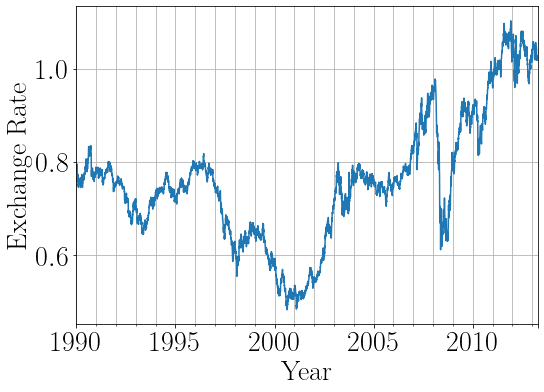
\includegraphics[width=\linewidth]{./img/exchange_rate_zoomed_2.png}
  \caption{Exchange rate of two currencies from 1990 to 2013.}
  \label{fig:example_timeseries}
  \endminipage\hfill
  \minipage{0.47\textwidth}
  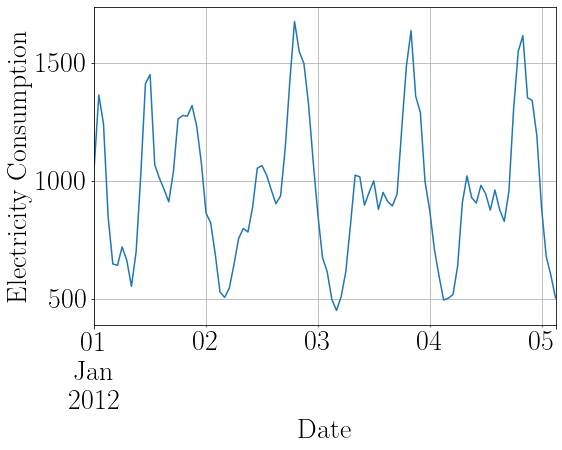
\includegraphics[width=\linewidth]{./img/electricity_zoomed_3.png}
  \caption{Household electricity consumption.}
  \label{fig:example_timeseries_electricity}
  \endminipage\hfill
\end{figure}

Timeseries which increase or decrease in value over a longer period of time is said to have a upward or downward \textit{trend}. If a timeseries has evenly distributed patterns such as the spikes in Figure \ref{fig:example_timeseries_electricity} the timeseries is said have a seasonal component with a frequency equal to the distance between the spikes. For the electricity timeseries this would be 24 as household electricity consumption follow the daily rythm of everyday life i.e. use more energy during the morning and evening with 24 hour intervals. If the timeseries exhibit spikes without a clear frequency, these are knowns as \textit{cycles} \cite{bauer2021libra}. The data which cannot be described by these features is known as the \textit{remainder} \cite{hyndman_forecasting_3rd}. Not all timeseries exhibit all of these patterns, for example, the timeseries in Figure \ref{fig:example_timeseries_electricity} does not display a trend.

\section{Time Series Decomposition}
Timeseries decomposition is the act of extracting features such as the seasonality and trend from timeseries data. This is often done in order to gain understanding of the data \cite{hyndman_forecasting_3rd}. While several methods of performing time series decomposition exists, one of the most powerful methods commonly used is STL decomposition \cite{hyndman_forecasting_3rd}. After a timeseries has been split into its constituents one can quantify the strength of the trend and seasonality apparent in the data. This is done through compairing the variances of the seasonality \(S\) and trend \(T\) with that of the residual \(R\). The strength of the trend \(F_t\) is then calculated according to Equation \ref{eq:strength_of_trend} and the strength of the seasonality \(F_s\) is calculated according to Equation \ref{eq:strength_of_seasonality}.

\begin{figure}[h]
  \[ F_t = max(0,1-\frac{Var(R)}{Var(T + R)}) \]
  \caption{Equation for calculating the strength of the trend of a timeseries.}
  \label{eq:strength_of_trend}
\end{figure}

\begin{figure}[h]
  \[ F_s = max(0,1-\frac{Var(R)}{Var(S + R)}) \]
  \caption{Equation for calculating the strength of the seasonality of a timeseries.}
  \label{eq:strength_of_seasonality}
\end{figure}

\section{Time Series Forecasting}
\label{sec_time_series_forecasting}
Time series forecasting is the art of predicting future trends of time series based on past observations. It is a key technology within many fields and is fundamental to the business decision process for many companies. Being able to interpret timeseries in order to predict future trends makes it possible to plan for the future. For example power generation companies can adjust the amount of electricity which should be generated to match the expected demand and banks could make informed decisions about possible investment opportunities. There are many methods of generating such predictions, ranging from the use of simple heuristics to complex machine learning methods \cite{hyndman_forecasting_3rd}. An overview of how to use deep learning to generate such forecasts is presented in Section \ref{sec:deep_learning_methods} and several state of the art forecasting models are presented in Section \ref{algorithms}.

Time series forecasting differs from common machine learning tasks such as image recognition or language processing in that predictions are not binary. More specifically, in time series forecasting a prediction is expected to be a close estimate of future values. Thus, quantifying the magnitude of the error from the ground truth is of importance in order to properly evaluate the accuracy of a forecasting model. This is commonly done by calculating an error metric, the choice of which varies depending on what is being forecasted and on preference of the forecasting practitioner. \cite{hyndman_forecasting_3rd,hyndman_measuring_nodate, willmott_advantages_2005} In Section \ref{subsec:error_metrics} some such error metrics are presented.

Forecasts often comes in one of two forms; probabilistic forecasts or point forecasts. A point forecast is a forecast which consist of only one estimation of future values. This estimation could be either a single point in time or a series of points for several different timesteps. In Figure \ref{fig:example_timeseries_forecast_point} an example of a point forecast for several timesteps can be seen. Point forecasts has the disadvantage that they do not confer how accurate they are which may lead to prectitioners being overly confident in the forecasts. This has historically caused several issues and more recently with covid-19 where over relying on point forecasts led to overly drastic measures for governments and hospitals \cite{IOANNIDIS2020}. Probabilistic forecasts such as the one in Figure \ref{fig:example_timeseries_forecast_probabilistic} includes this information by generating prediction intervals of the forecasts.

\begin{figure}[htb]
  \centering
  \minipage{0.5\textwidth}
  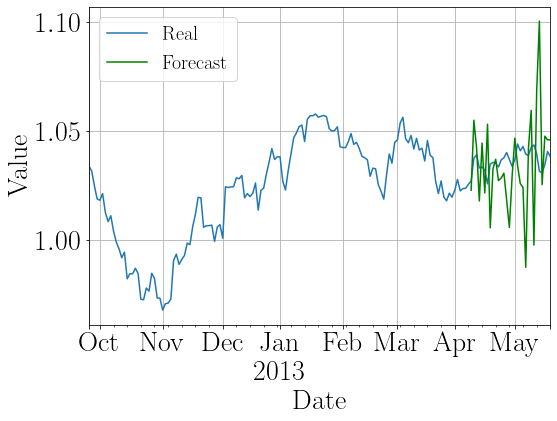
\includegraphics[width=\linewidth]{./img/exchange_rate_point_forcast.png}
  \caption{Point forecast}
  \label{fig:example_timeseries_forecast_point}
  \endminipage\hfill
  \minipage{0.5\textwidth}
  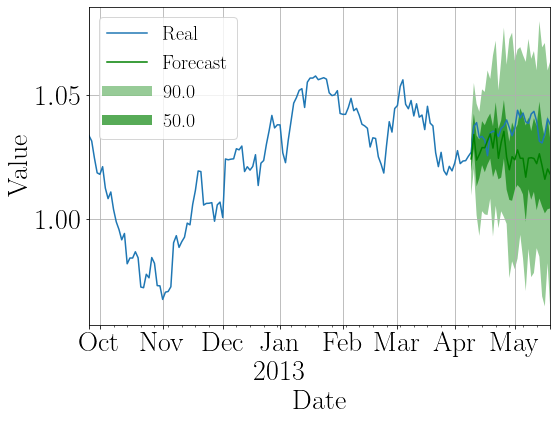
\includegraphics[width=\linewidth]{./img/exchange_rate_prob_forcast.png}
  \caption{Probability forecast}
  \label{fig:example_timeseries_forecast_probabilistic}
  \endminipage\hfill
\end{figure}

Many methods exist for generating forecasts on timeseries data, two common groups of these are machine learning based methods and trivial methods. A trivial forecasting method would be, for example, to predict that the next value should be the same as the last recently observed value or the average of the last N observations. For certain timeseries, trivial methods perform competitively and as such these are often held as a baseline to which new forecasting methods are being compared too. Some more complex methods include those based on regression analysis such as linear regression or autoregressive models such as ARIMA \cite{hyndman_forecasting_3rd}. Autoregressive models are a subset of regression models where the temporal ordering of the datapoints matter. I.e. autoregressive models use past observations to predict future values.

Lately, inspired by the successful use of neural networks in other domains, several neural network based approaches for time series forecasting have been introduced. Early implementations such as simple multi-layered perceptrons did not perform competitively with the more classical approaches such ARIMA. However modern deep learning models such as DeepAR \cite{salinas_deepar_2019} and MQCNN \cite{wen_multi-horizon_2018} have reported highly competitive accuracies.

Forecasting models for forecasting can also be split into further sub families such as whether they are local or global models. Local models are trained on individual time series while global models are trained on all time series in the training set. Essentially for a dataset with N timeseries, if using local models, one will have N individually trained models. If the algorithm would be a global model then only a single model would be used for all N timeseries in the dataset. Generally speaking, local models performs well for timeseries with much historical data. However for short or new timeseries, local models often perform poorly due to the inability to train the model on sufficiently large amounts of data points. This is known as the cold start problem. Since global models train on the entire dataset across all timeseries, the length of any individual timeseries has less of an impact. I.e. generally global models suffer less from the cold start issue as the global model can use data from other timeseries as a basis for its predictions \cite{wang_deep_2019}.

So far, we have seen the time series forecasting problem as generating a forecast from a single timeseries for example predicting future temperatures based on previously recorded temperatures. Predicting using singular timeseries such as this is known as univariate forecasting. Another family of forecasting solutions leverage related timeseries when making predictions. For example temperatures may depend on cloud coverage or the hours of sunlight. Algorithm which leverage information from related timseries are known as multivariate algorithms. The benefits of multivariate forecasting is that trends or patterns can be identified using these related timeseries in order to improve the accuracy for the target variable. For example, the temperature is higher whenever there is a large amou8nt of sun hours and no clouds.

\section{Evaluating Forecasting Performance}
\label{sec:evaluating_performance}
If a model generates forecasts it is important to be able to quantify how good or bad its predictions are. This is generally done via a process called backtesting. When backtesting, first the algorithm is trained on a dataset, thereafter, the trained algorithm generates predictions on a test dataset. The generated predictions from the algorithm are then compared to the ground truth and a suitable error metric quantifying how wrong the prediction was from the expected value is calculated.

In other machine learning domains such as image recognition, the datasets used for training the models are disjoint from the test datasets. However, in the domain of time series forecasting this is not the case. Generally the train set contains the same time series as in the test set except for the last couple of data points for each time series. The number of removed data points is commonly the number of timesteps that a model should predict \cite{hyndman_forecasting_3rd}. In Figure \ref{fig:train_test_split} a train test split is presented of a time series with six data points. In this example, a forecasting algorithm should predict one timesteps into the future, thus, the last datapoint would be removed and the train set would contain five data points while the test series would contain six.

\begin{figure}[htb]
  \centering
  \minipage{1\textwidth}
  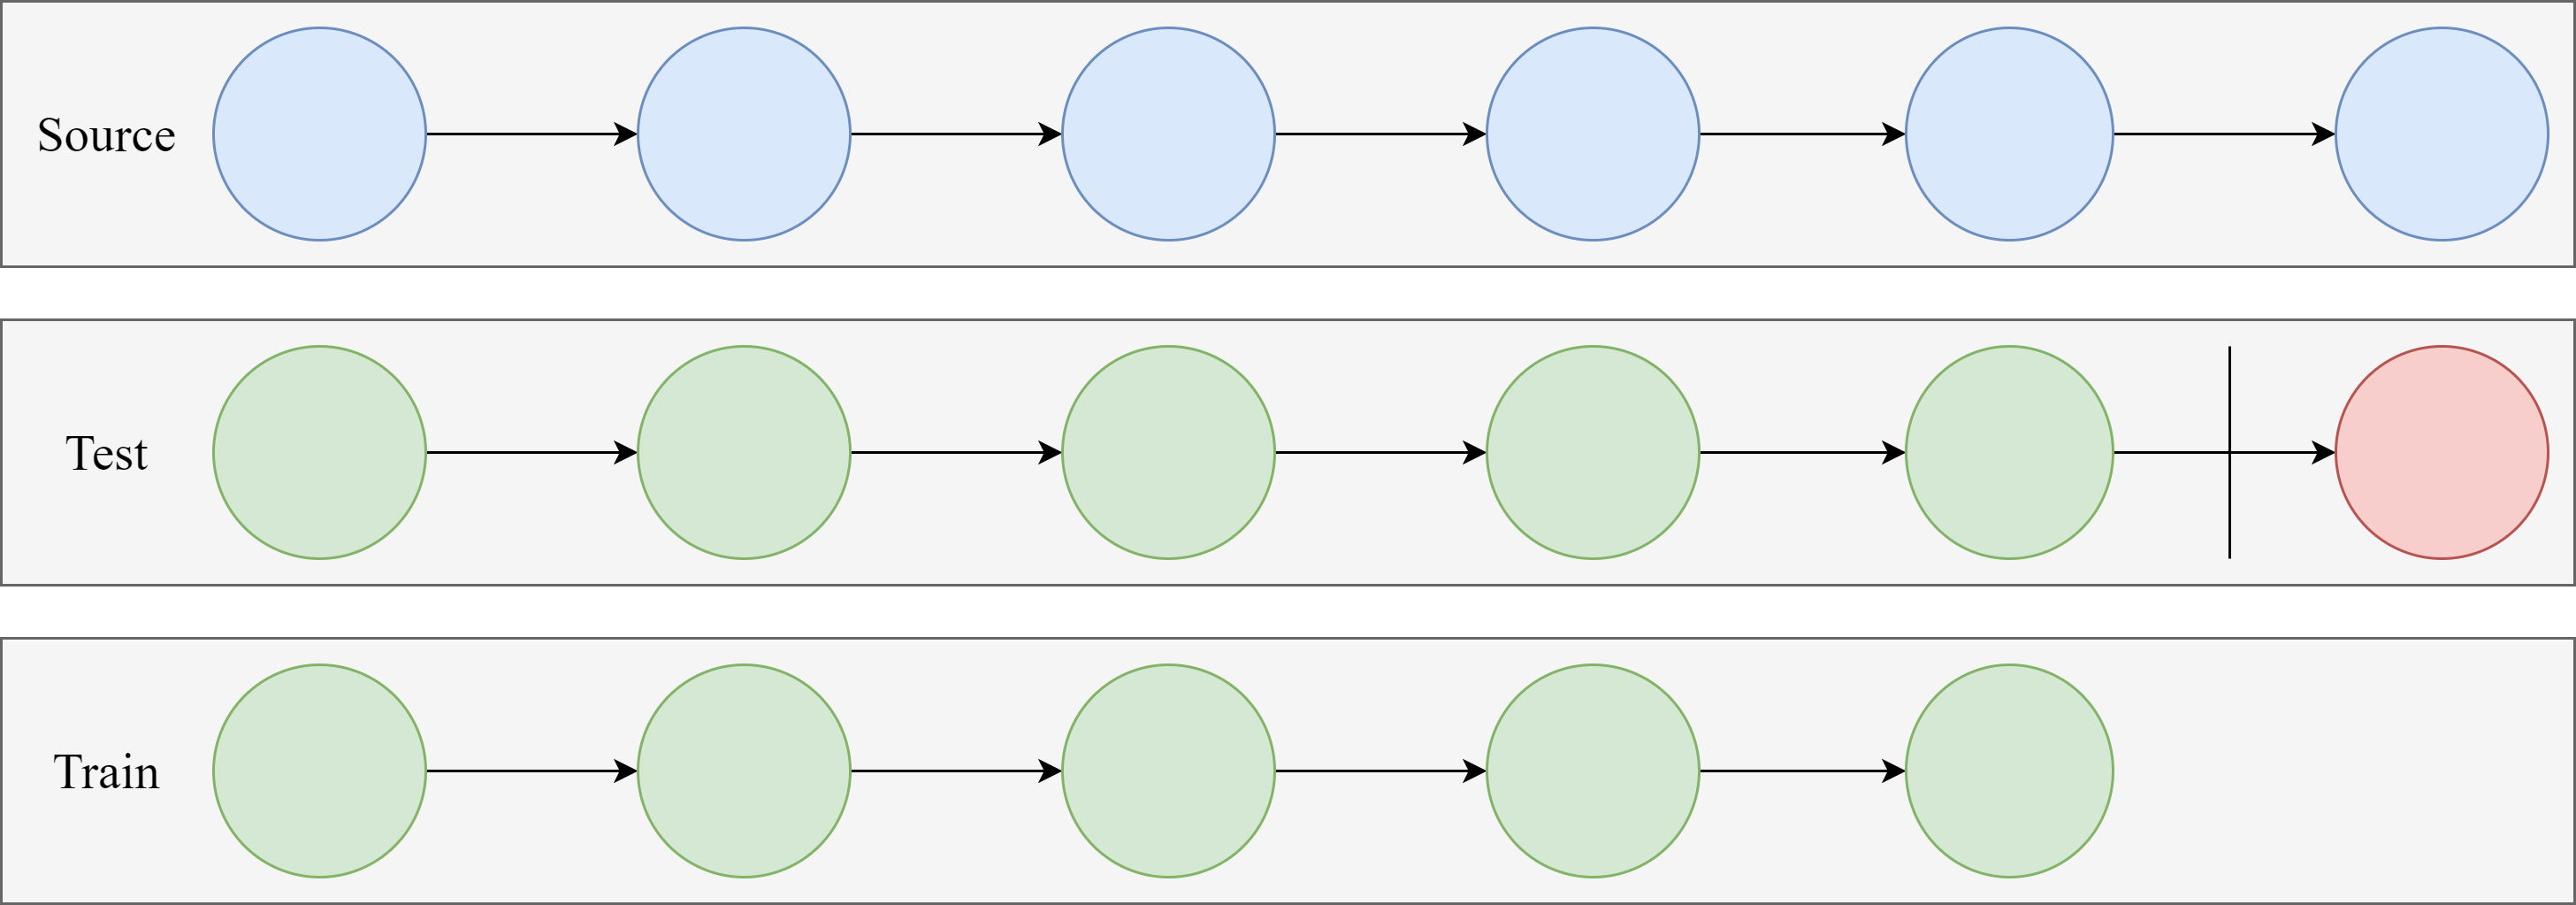
\includegraphics[width=\linewidth]{./img/train_test_split.png}
  \caption{An example train test split of a time series with six datapoints. The red circle is the datapoint which prediction will be compared to.}
  \label{fig:train_test_split}
  \endminipage\hfill
\end{figure}


A popular method of increasing the amount of test data is to make the test dataset contain multiple copies of each time series where each one is successively shorter. The train dataset would contain the shortest of the truncated time series truncated one additional time. This process is called K-fold cross validation but is also known as forecasting on a rolling origin or time series cross validation. Performing a 3-fold cross validation on a dataset containing one time series of length six timesteps would result in a dataset containing three time series. An example of this is shown in Figure \ref{fig:k_fold_validation}. The advantage of the larger test dataset generated by this approach is that the performance of a model can be more accurately determined as it is excercised on more unseen data \cite{hyndman_forecasting_3rd}.

\begin{figure}[htb]
  \centering
  \minipage{1\textwidth}
  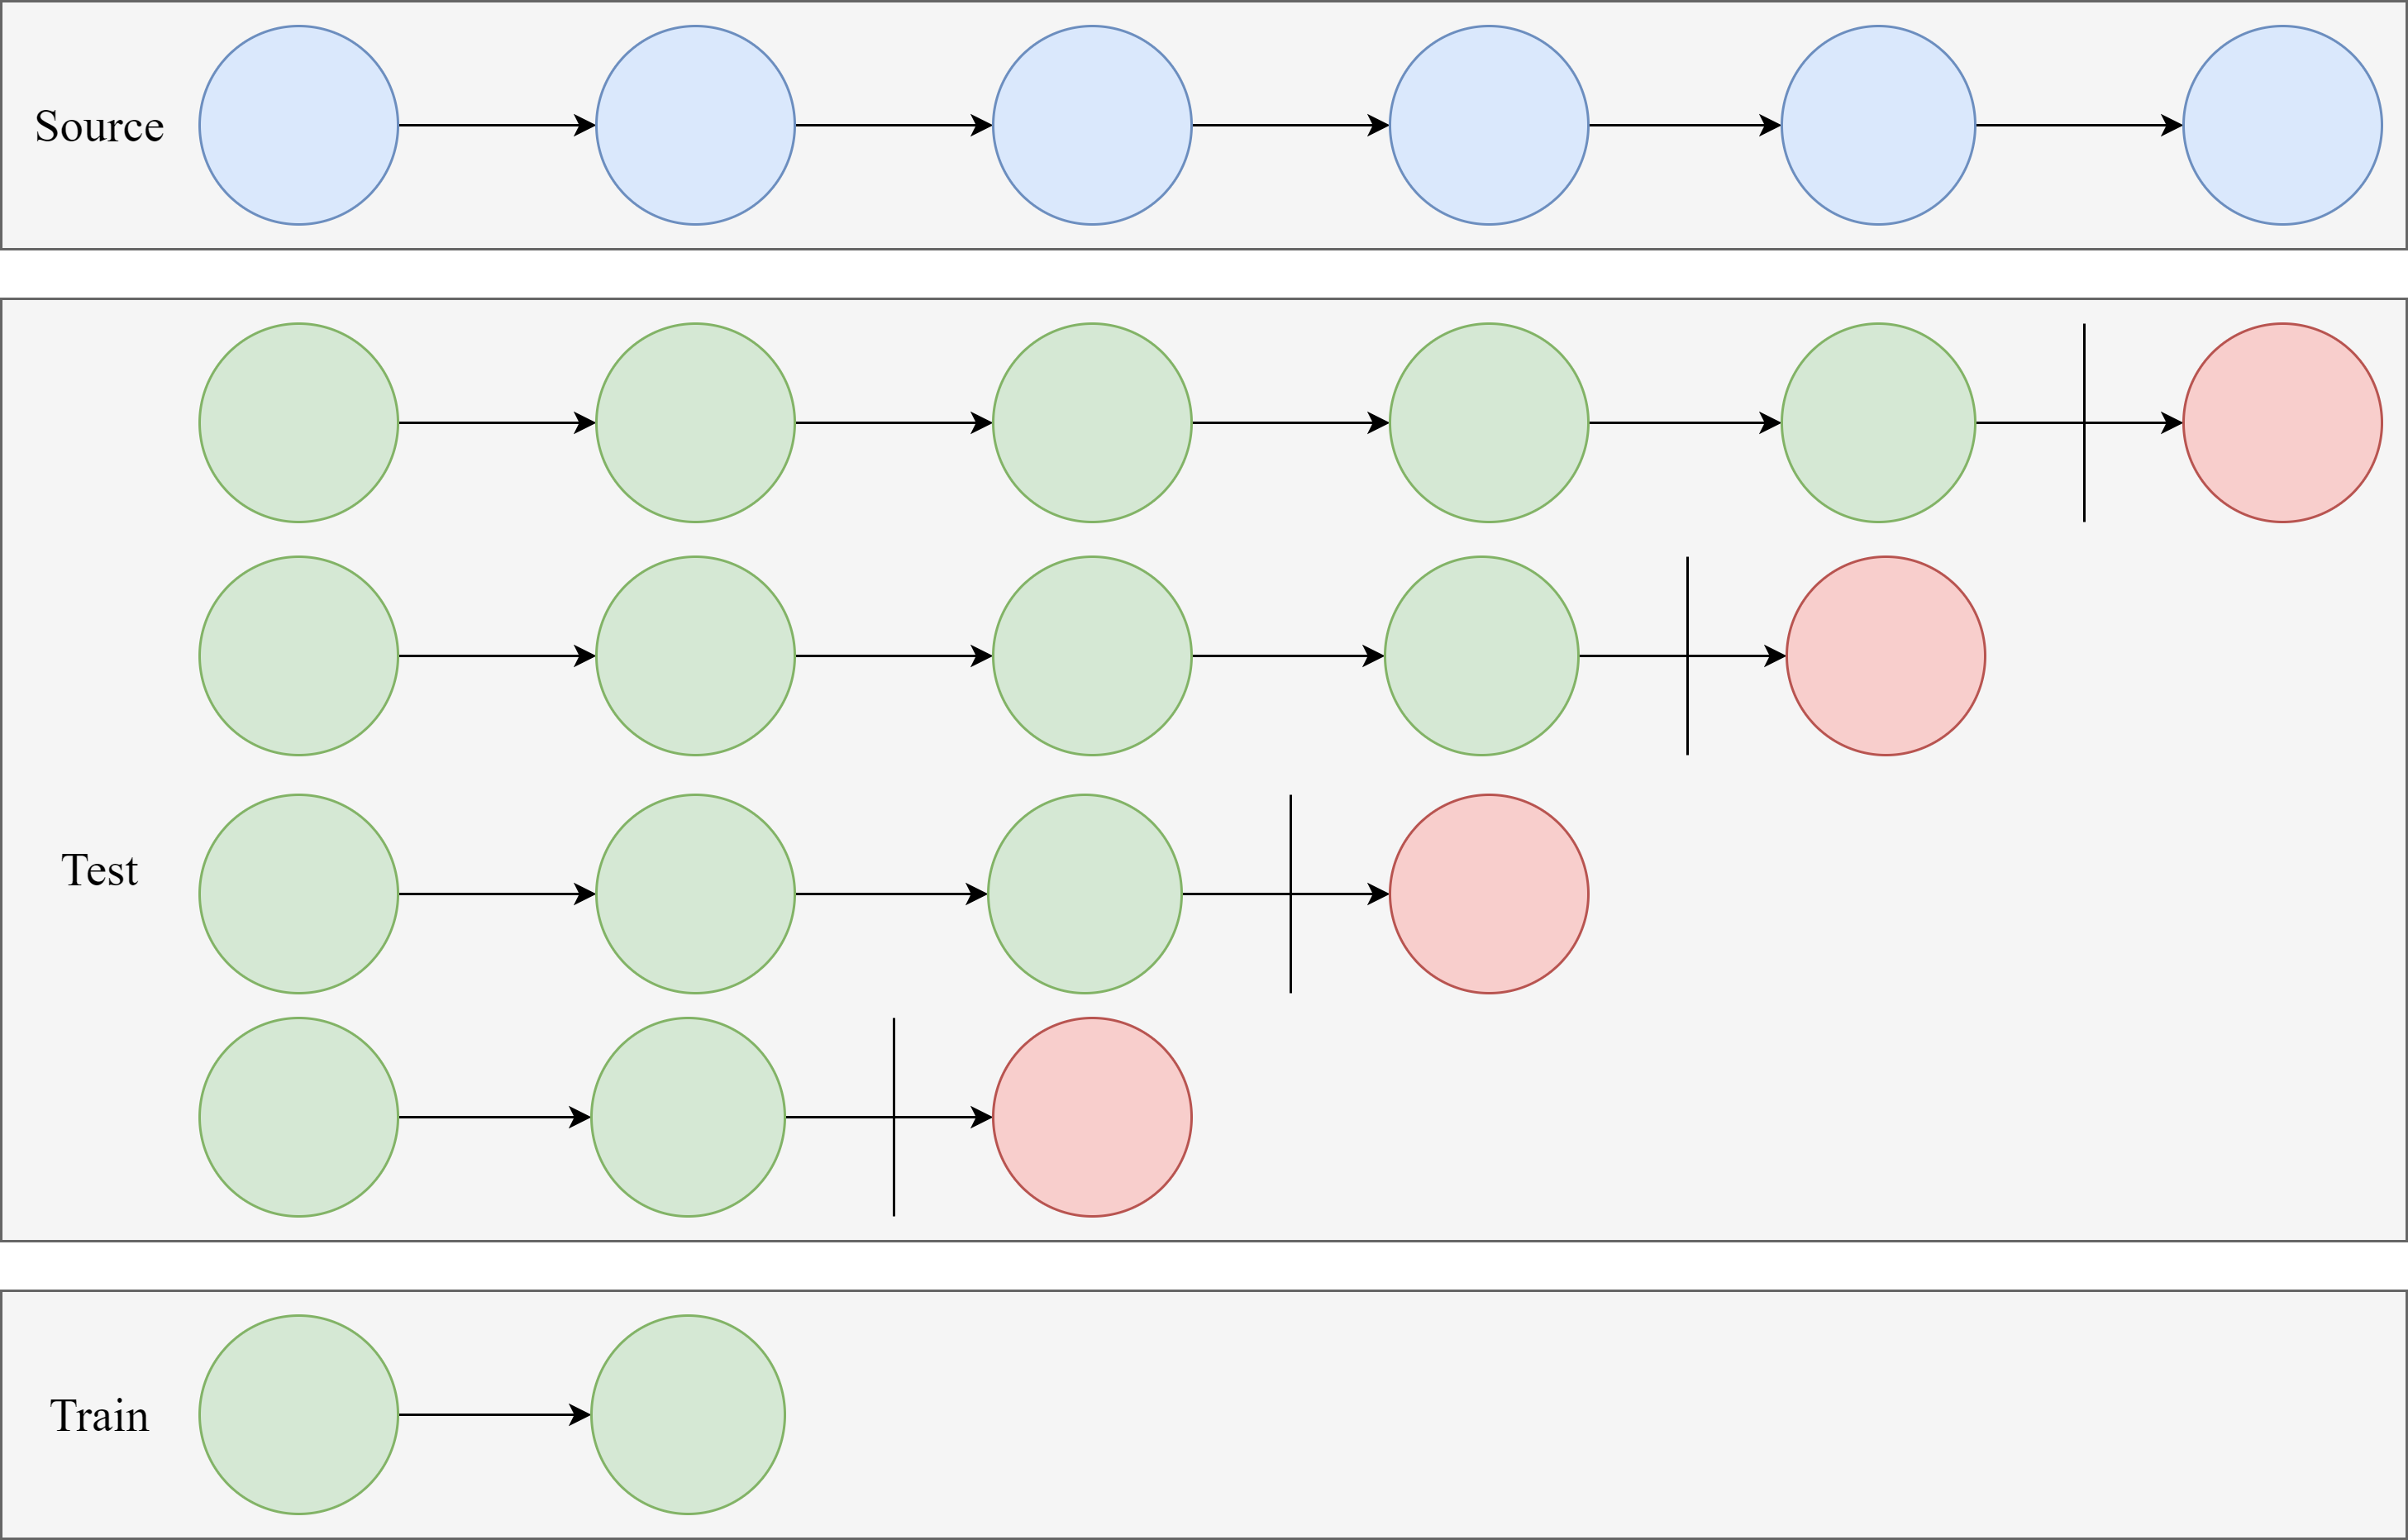
\includegraphics[width=\linewidth]{./img/k_fold_validation.png}
  \caption{Example of a four fold cross validation dataset split. The red circles are the datapoints which predictions will be compaired to. Worth noting is that the train dataset here only has one timeseries of length two, i.e. one less than the shortest timeseries in the test dataset. This example assumes a prediction length for the dataset of one datapoint.}
  \label{fig:k_fold_validation}
  \endminipage\hfill
\end{figure}


\subsection{Error Metrics}
\label{subsec:error_metrics}
When a forecasting model generates predictions on a timeseries, one needs to be able to quantify the error of the prediction from true observed values. In order to do this many different error metrics exists each with its own benefits and drawbacks. Often the choice of metric is dependent on data, and business application where the prediction will be used. In this section some of the error metrics which are commonly occurring in literature are presented. These metrics are calculated automatically when performing a backtest in Gluon-TS, see \ref{subsec:gluonts_overview} for details about this process. Note that only a subset of the metrics available in Gluon-TS is presented here to form a basis for subsequent chapters.

Error metrics for forecasting can generally be split into three different categories: scale-dependent, scaled and percentage based \cite{hyndman_forecasting_3rd}. Within each of these categories multiple different metrics exists. The remainder of this section describes some common error metrics within each category along with pros and cons and how they are calculated. For the rest of the thesis, a forecast is referred to as \(\hat{Y}\) and the expected values are referred to as \(Y\).

\subsubsection{Absolute Error}
The absolute error is calculated as the distance between the predicted value and the ground truth. An absolute error is positive and a value of 0 is optimal. It is an intuitively simple error, thus it can easily be understood and discussed when comparing algorithms.

However intuitive the absolute error is, there is a a key issue with this error and that is that it is scale dependent. I.e. the greater the values of the dataset being predicted on, the larger the absolute error will be. This makes it impossible to compare the accuracy of an algorithm across different datasets unless they have the same scale. \cite{hyndman_forecasting_3rd} Furthermore, scale dependent metrics such as these may not be suitable even for comparing between timeseries within a single dataset. Imagine a dataset such as the electricity dataset (see Table \ref{tab:datasets}) where each timeseries is the electricity consumption from a household. One household may contain many people and appliances while another may be a factory full of equipment with high power demands. These two timeseries would have two very different scales thus making it hard to compare the accuracy of the predictions.

\begin{figure}[h]
  \[Absolute Error = \sum|Y - \hat{Y}|\]
  \caption{Equation for calculating the absolute error}
  \label{eq:abs_error}
\end{figure}

\subsubsection{Root Mean Squared Error - RMSE}
\label{sec:RMSE}
The root mean squared error is another scale dependent error such as the absolute error. RMSE is calculated by taking the square root of the mean of the squared error. The RMSE thus punishes larger errors more than smaller errors. The RMSE is more complicated to interpret than for example the Absolute Error due to the non-linear nature, despite this, RMSE is widely used in practise \cite{hyndman_forecasting_3rd,gluonts-github}.

\begin{figure}[h]
  \[RMSE = \sqrt{mean((Y - \hat{Y})^2)}\]
  \caption{Equation for calculating RMSE}
  \label{eq:RMSE}
\end{figure}

\subsubsection{Mean Absolute Percentage Error - MAPE}
Percentage based errors such as the Mean Average Percentage Error normalizes the errors between 0 and 1 thus MAPE can be compared across datasets with different scales. While this is beneficial, MAPE suffer from other issues. For example MAPE becomes infinite or undefined if the ground truth is 0 for any parts of the prediction. Further issues exists for example that it penalizes negative errors more than positive errors. These issues has lead to variations of MAPE to be created such as Symmetric MAPE \cite{hyndman_forecasting_3rd,gluonts-github}.

\begin{figure}[h]
  \[MAPE = mean(\frac{|Y - \hat{Y}|}{|Y|}))\]
  \caption{Equation for calculating MAPE}
  \label{eq:MAPE}
\end{figure}

\subsubsection{Mean Absolute Scaled Error - MASE}
MASE is a metric which takes the average error across all timeseries and scale is based on the error from a reference forecasting. An example a model which MASE uses for reference would be the Naive2Estimator detailed in Section \ref{model:naive2}. Scaling the forecasting error in this way causes the MASE metric to be scale independent which makes it suitable when comparing across datasets. A MASE of 1 corresponds to that the algorithm under test is equally good as the naive model. A MASE below 1 means that the current model performs better than the naive model while a MASE above 1 means that the model performs worse than the naive baseline model \cite{hyndman_forecasting_3rd,gluonts-github}.

In certain scenarios, for example if the reference model would result in a perfect prediction a division by zero would occur and MASE would tend towards infinity. This is a major drawback of the MASE metric which renders it unusable for certain datasets.

In equation \ref{eq:MASE} the denominator is the mean error of a seasonal naive model. \(Y_t\) means the value at time \(t\) and \(Y_{t-m}\) means the value of the timeseries at the previous period, i.e. if the expected seasonality is 24h \(Y_{t-m}\) would become the value 24 timesteps previously.

\begin{figure}[h]
  \[MASE = \frac{mean(|Y - \hat{Y}|)}{mean(|Y_t - Y_{t-m}]|)}\]
  \caption{Equation for calculating MASE}
  \label{eq:MASE}
\end{figure}

\subsubsection{Mean Scaled Interval Score - MSIS}
\label{sec:msis}
Since probabilistic forecasts do not generate point predictions but prediction intervals these can also be scored in regards to how often these contain the true values \(Y\). The MSIS metric penalizes wide prediction intervals in two ways. First, the absolute width of the prediction intervals is penalized. Secondly, the distance from the edge of the prediction interval from the expected value \(Y\) is penalized. Thus smaller more accurate and consistent prediction intervals are encouraged \cite{makridakis_m4_2020}. In Equation \ref{eq:MSIS} \(\hat{Y_u}\) is the upper limit of the forecast prediction interval and \(\hat{Y_l}\) is the lower boundrary. The \(\alpha\) parameter is the significance level used, this is commonly set to 0.05 to evaluate the 95\% prediction intervals \cite{makridakis_m4_2020,gluonts-github}. The \(I(x)\) function is the indicator function which is 1 if \(\hat{Y}\) is within the prediction interval and 0 otherwise. The denominator used in Equation \ref{eq:MSIS} is the mean seasonal error, i.e. the same denominator for the MASE metric. This division makes the MSIS metric scale independent \cite{gluonts-github,makridakis_m4_2020}.

\begin{figure}[h]
  \[msis = \frac{mean(\hat{Y_u} - \hat{Y_l} + \frac{2(\hat{Y_l}-Y)}{\alpha}I(Y<\hat{Y_l}) + \frac{2(Y-\hat{Y_u})}{\alpha}I(Y>\hat{Y_u}))}{mean(|Y_t - Y_{t-m}]|))}\]
  \caption{Equation for calculating MSIS}
  \label{eq:MSIS}
\end{figure}

\section{Deep Learning Forecasting Methods}
\label{sec:deep_learning_methods}
Neural Networks (NN) have in recent years been successfully applied in many different domains such as image recognition and natural language processing. However, within the field of forecasting NN based approaches has performed subpar compared to more traditional statistical methods \cite{m3_competition,makridakis_m4_2020,oreshkin_n_beats_2020, other_thesis}. This relative inefficiency between NN based approaches and classical methods and the success of NN in other domains has resulted in much research being made in improving tools and NN based models for forecasting \cite{gluonts_paper}.

A simple neural network, similar in architecture to the network described in Section \ref{algo:simplefeedforward} is presented in Figure \ref{fig:simplefeedforward}.

\begin{figure}[htb]
  \centering
  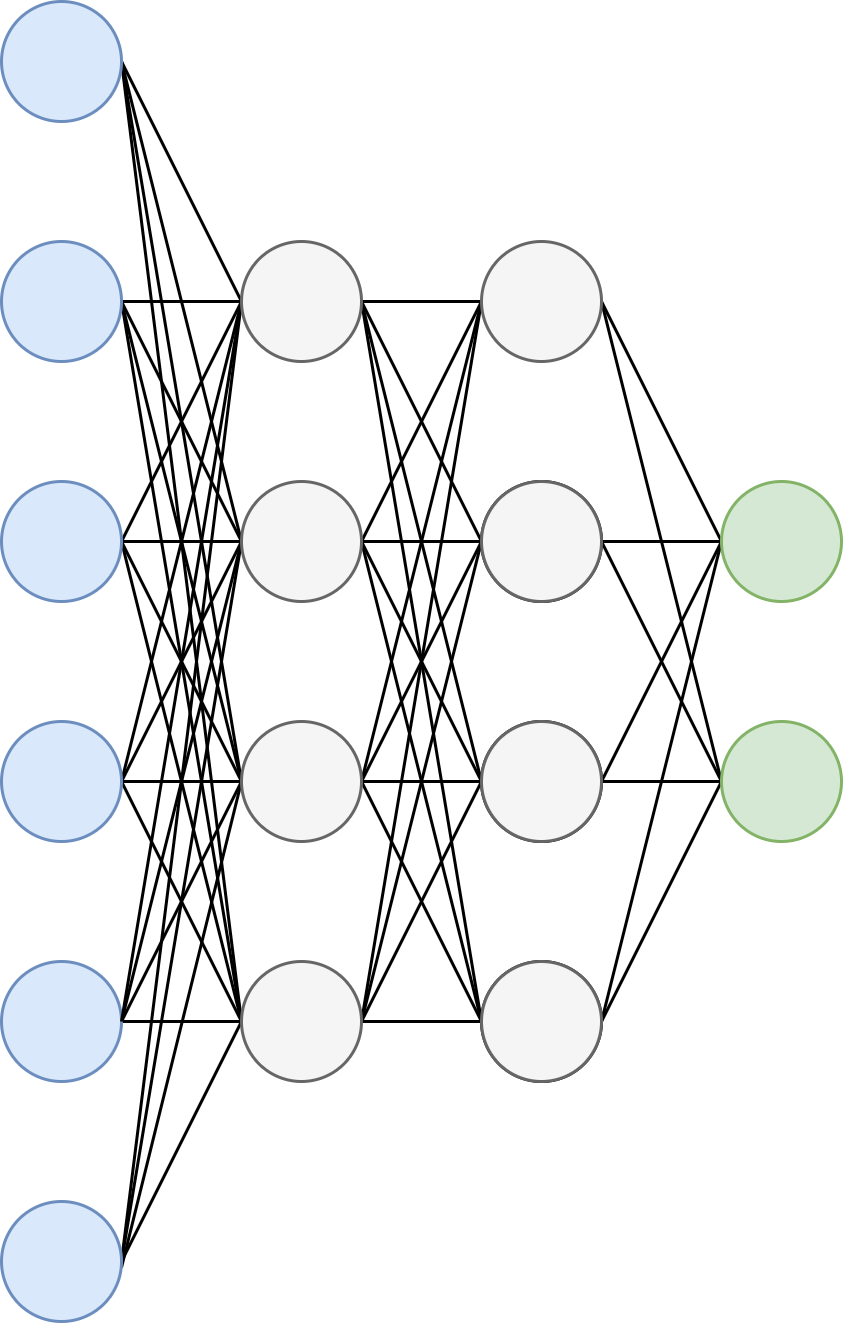
\includegraphics[width=0.5\linewidth]{./img/simplefeedforward.png}
  \caption{A simple neural network for forecasting based on the SimpleFeedForwardEstimator in Section \ref{algo:simplefeedforward}.}
  \label{fig:simplefeedforward}
\end{figure}
\clearpage

This very small network consists of four fully connected layers of different sizes with six input nodes, two fully connected hidden layers with four nodes each, and an output layer of two nodes. In this network, the input layer (marked in blue) has the same amount of nodes as the number of timepoints in the past which the network should make use of. This is will in the remainder of the thesis be called the \textit{context length} of the network. The output nodes (in green) for this network produce a prediction of two timesteps. Thus this network has a \textit{prediction length} of two timesteps. The context length and the desired prediction length are often exposed as hyperparameters for time series forecasting algorithms since they vary between datasets.

An issue with the simple network in Figure \ref{fig:simplefeedforward} is that each timestep in the forecast is not influenced by the previous one. i.e. the prediction at timestep \(N\) does not depend on the prediction at timestep \(N-1\). In real life scenarios, timeseries data often has a temporal dependency, for example, the temperature two days from now is affected by the temperature of tomorrow. This dependency is lost in simple neural network architectures such as this one. An alternative neural network architecture which can make use of temporal effects is known as a Recurrent Neural Network (RNN).

RNNs reuse the output of their nodes as inputs for the next iteration of the algorithm. This recurrent link causes previously seen values in the sequence to be represented in a hidden internal state. While this makes RNNs suited for use with sequential data such as time series, they become hard to train successfully as long term dependencies are lost \cite{bengio1994learning}. One of the most successful techniques for use in RNNs to solve this is the Long Short-Term Memory (LSTM) node architecture. LSTM nodes enables RNNs to remember previously seen data for longer and forget or ignore parts of it \cite{sherstinsky_fundamentals_2020}.

Some issues with NN based approaches is that they require a large amount of data to be trained on properly. This is due to the fact that NNs are prone to overfit which makes them unable to generalize well to new data \cite{srivastava_dropout_2014}. Despite this, NN has several advantages over classical approaches such as the capability to learn non-linear patterns from the data. Additionally, NN models are capable of cross learning between related time series without the need of manual feature extraction \cite{smyl_hybrid_2020}.

\subsection{Sources of Randomness}
\label{subsec:sources_randomness}
Neural networks heavily rely on random processess to function and thus randomnes is introduced at several points in a forecasting workflow. Some randomness can be introduced whenever an neural network is initialized as the weights and biases of a networks often are set randomly. Similarly, when training a neural network randomness can be introduced if optimization techniques such as dropout is used as dropout randomly sets weights in the network to 0 at certain points in the training loop which causes the algorithm to be less prone of overfitting the data \cite{srivastava_dropout_2014}. Even the method used for training neural networks, stochastic gradient descent introduces randomness.

Deep NNs are notoriously slow to train when compared to many other methods, thus lowering the time spent for training and inference is often done by parallelizing algorithms such that they run on several threads on a CPU or on hardware accelerators such as GPUs, FPGAs or ASICs. The execution speed of a forecasting model is thus highly dependent on what hardware the models are running on, however the hardware configuration also impacts the variance of the accuracy of ML models \cite{zhuang2021randomness}. Parallelization of an algorithm often introduces a larger amount of data shuffling which impacts the rate of convergence of an algorithm. Parallelizing a forecasting model may make it unstable so that it cannot converge as will be shown in chapter \ref{cha:chapter6}. Due to this it is important that the hardware used when training and tuning forecasting models is presented in detail so that results can be properly reproduced \cite{pineau2020improving}.

A common method for reducing the randomness associated with ML models is to fix the seed used by the random number generator to a known number. While this removes randomness from for example random initializations or from backpropagation \cite{beam2020challenges}, other sources of randomness such as that introduced by the hardware or the OS remain. Furthermore, fixing the seed can be seen as an additional hyperparameter which needs to be tuned as it directly impacts the predictive performance of forecasting methods. While there are some major benefits of fixing the seed, there are also drawbacks. For example,luck becomes a factor in what accuracy can be expected for an algorithm. I.e. the accuracy of a model may seem highly competitive while if another seed would be used the accuracy of the model could change significantly \cite{beam2020challenges}. In real life usecases such as when forecasting are used in companies or organizations, setting the seed may be beneficial or even necessary in order to optimize its performance for an individual task. In research however, setting the seed without reporting what it was can bias results and make them technically irreproducible \cite{beam2020challenges,pineau2020improving,bouthillier2021accounting}.

One method of lowering the variance of machine learning methods is to use ensambles of forecasting methods as per the Bootstrap AGGregatING (Bagging) technique \cite{buhlmann2002analyzing}. An ensamble is a set of multiple different ML models with slightly different configurations which are all trained in parallel.Bagging extends this such that a the input dataset is randomly sampled to create multiple independent datasets. Each model is then trained on one of these datasets and their forecasts are then combined via some voting or weighting scheme \cite{buhlmann2002analyzing}. While bagging is often associated with decision trees they are also suitable for use with deep learning forecasting models such as the N-BEATS Ensamble Estimator discussed in Section \ref{algo:nbeats}.

K-fold cross validation which was discussed in Section \ref{sec:evaluating_performance} can also lower the variance of forecasting algorithms as it introduces multiple different train-test splits from a single dataset \cite{buhlmann2002analyzing}.

\section{Benchmarking}
\label{sec:related_work}

Backtesting is a fundamental part of benchmarking, however benchmarking is also concerned with ensuring that different models can be fairly and reproducibly compared to each other \cite{huang_benchmarking_2019}. In other domains of machine learning several benchmarking solutions exists, most notably MLPerf \cite{mattson_mlperf_2020}, MLBench \cite{noauthor_mlbench_nodate}, DLBS \cite{vassilieva_deep_nodate} and UCR \cite{dau2019ucr}. Despite the success of benchmarks in other ML domains no established “go-to” benchmark exists in the domain of time series forecasting \cite{huang_benchmarking_2019}.

Attempts has been made to create such a benchmark, one such example is \textit{Libra} \cite{bauer2021libra} which uses custom datasets containing timeseries sampled from various well known datasets. The sampling methodology used in Libra was aimed to create datasets with a high amount of diversity between the timeseries. Due to this diversity, the datasets in Libra are not suitable for global forecasting models as they are highly unrelated. In a nutshell, Libra focuses on benchmarking the accuracy and time-to-result for univariate forecasts generated by local models.


\begin{table}[h]
  \begin{tabularx}{\textwidth}{|l|c|c|c|c|X|}
    \hline
    Name    & TS & Integration    & DS & Focus & Info                                                                    \\
    \hline
    \hline
    Libra   & X  & R              & X  & A, S  & Diverse datasets for univariate local models                            \\
    \hline
    UCR     & X  & CSV            & X  & A     & Dataset repository with reference accuracies.                           \\
    \hline
    MLPerf  &    & Docker, CLI    &    & S     & Benchmarking for hardware and ML frameworks                             \\
    \hline
    PMLB    & X  & Python, R      & X  & -     & Dataset repository with 298 datasets for regression and classification. \\
    \hline
    MLBench &    & Kubernetes     &    & S     & For distributed ML frameworks                                           \\
    \hline
    DLBS    &    & Docker, Python &    & S     & Benchmarking for hardware and ML frameworks                             \\
    \hline
  \end{tabularx}
  \caption{Overview of six benchmarking suites for ML, the column marked TS depicts whether they support time series forecasting and the DS column is whether they offer custom datasets. A is shorthand for  Accuracy and S for Speed.}
  \label{tab:benchmarking_suites}
\end{table}

Instead of using benchmarking suites when comparing forecasting models, new forecasting solutions are instead pitted against each other in forecasting competitions. The Makridakis Competitions organized by Makridakis Spyros et.al. are the most well known of these and has at the time of writing undergone five iterations; the M1 in 1983 \cite{makridakis1987confidence}, M2 in 1982 \cite{makridakis1993m2}, M3 in 2000 \cite{m3_competition}, M4 in 2018 \cite{makridakis_m4_2020} and the M5 competition in 2020 \cite{m5}. These competitions have been highly impactful for the field of forecasting and has been the norm to which researchers compare too. However it was not until the M3 competition that NN based forecasters were included. These performed poorly compared to the non-NN algorithms which can partly be attributed to the limited size of the M3 dataset of 3003 timeseries \cite{m3_competition}. This shortcoming of the M3 dataset lead to the creation of the M4 competition which had a similar but much larger dataset containing 100 000 timeseries \cite{makridakis_m4_2020}. Despite this, the findings of the M4 competition was inline with that of the M3 competition in that approaches purely using NN performed worse than even simple models. However, the M4 competition winner was a hybrid approach which combined RNNs with classical models. The latest competition, the M5, was focused on retail sales forecasting and found for the first time that ML based solutions, primarily Gradient Boosting Trees but also NN approaches such as DeepAR outperformed classical statistical methods \cite{m5}.

In 2015 a thesis comparing forecasting solutions was published with the topic: \textit{Benchmarking of Classical and Machine-Learning Algorithms (with special emphasis on Bagging and Boosting Approaches) for Time Series Forecasting} \cite{other_thesis}. This thesis put the focus on performing a thorough dataset analysis and evaluating 14 algorithms on three real world datasets; Tourism, M3 and the NN5 \cite{NN5_website}. Each algorithm was evaluated on multiple versions of each of these datasets with different preprocessing applied to them. In addition to evaluating the algorithms on the three real life datasets, a simulation study on artificial data was conducted. The purpose of this was to identify strengths and weaknesses of the algorithms for timeseries with simple characteristics such as only having trend or seasonality.

It is unclear whether time series cross validation was used as well as how many times each algorithm was executed. Further, as the title suggests there was little emphasis on deep learning methods and only a very simple neural network, similar to the one presented in Figure \ref{fig:simplefeedforward} was used. This neural network performed worse than the naive approach for all datasets except for on NN5 \cite{other_thesis}.



\subsection{Reproducibility}
\label{sec:reproducibility}
The ability to reproduce scientific results within the field of machine learning has been a hot topic in recent years with major conferences such as NeurIPS announcing dedicated reproducibility programs \cite{pineau2020improving}. Certain fields of ML research such as within healthcare is reportedly in a \textit{reproducibility crisis} \cite{beam2020challenges, mcdermott2019reproducibility}. Surveys conducted in 2018 reported that only 63\% of 255 ML publications could be reproduced and only 4\% of them could be reproduced without the original authors assistance \cite{pineau2020improving}. Another survey in Nature sent out to more than 1500 scientists from various diciplines in 2016 reported that 50\% researchers failed in reproducing even their own experiments \cite{baker20161}. Also Makridakis et.al., the organizers of the M-competitions, urged researchers to improve the reproducibility of their work. The following is a quote from their paper summarizing the M4 competition: \textit{"We believe that there is an urgent need for the results of important ML studies claiming superior forecasting performance to be replicated/reproduced, and therefore call for such studies to make their data and forecasting algorithms publically available, which is not currently the case"} \cite{makridakis_m4_2020}.

There are multiple methods of defining reproducibility. Pineau et.al. defined reproducibility as being able as \textit{re-doing an experiment using the same data and same analytical tools} \cite{pineau2020improving}. This definition aligns with that of Beam et.al. however, they point out that reproducibility is not concerned with the validity of the claims of a paper, only that practical results can be recreated \cite{beam2020challenges}. McDermott et.al. further specifies the term reproducibility into three parts \textit{technical}, \textit{statistical} and \textit{conceptual}. For technical reproducibility, the code and datasets used should be made publically available and in order to be statistically reproducible, the variance of the results should be published. To be conceptually reprodicble, it was important that multiple datasets should be used for the comparisons \cite{mcdermott2019reproducibility}.

In addition to the requirement that code and datasets should be made available, Pineau et.al. suggested that standardized tools for supporting reproducibility should be developed and that any metrics used should be sufficiently specified. Furthermore it was argued that encapsulation tools such as Docker should be used as these would remove OS and dependency related issues \cite{pineau2020improving}. This would also resolve issues pertaining to different versions of code being used \cite{beam2020challenges}. The random seed which was discussed in Section \ref{subsec:sources_randomness} is also an important value which should be reported as it can drastically affect the performance, especially for neural network based models \cite{beam2020challenges, bouthillier2021accounting}. Increasing the use of statistical tests is another key aspect for improving the reproducibility \cite{mcdermott2019reproducibility}. In addition to this forecasting models should be executed multiple times with as much variation as possible between each run to further improve the accuracy and the statistical reproducibility of the results
\cite{bouthillier2021accounting}.

A summary of the requirements for achieving reproducibility is presented in Table \ref{tab:reproducibility}.

\begin{table}[h]
  \centering
  \begin{tabularx}{\textwidth}{|l|X|}
    \hline
    Type of reproducibility & Requirements                                                                                                                                                                               \\
    \hline
    \hline
    Technical               & Code and datasets should be publically available. If random seed is set it should be reported. Specific versions of code should be detailed and assets such as Docker containers provided. \\
    \hline
    Statistical             & Variance of results should be published and statistical tests should be used.                                                                                                              \\
    \hline
    Conceptual              & Multiple complimentary datasets should be used for the comparison.                                                                                                                         \\
    \hline
  \end{tabularx}
  \caption{Requirements for making ML workloads reproducible.}
  \label{tab:reproducibility}
\end{table}


\section{Gluon-TS}
\label{subsec:gluonts_overview}
Gluon-TS is an open source library which includes several deep learning algorithms, datasets and tools for building and evaluating deep learning forecasting methods \cite{gluonts-website,gluonts_paper,gluonts-github}. In Gluon-TS, the \textit{Estimator} class corresponds to the implementation of a forecasting method. An \textit{Estimator} can be trained on a dataset in order to generate a \textit{Predictor} object. This \textit{Predictor} can then ingest timeseries in order to produce forecasts for them.

In order to make it easy to evaluate the performance of an algorithm, Gluon-TS offers the \textit{backtest\_metrics} function. This function trains an \textit{Estimator} on a train dataset, the generated \textit{Predictor} is then used to generate predictions on a test dataset. Each of the timeseries in the test dataset will have the final \textit{N} datapoints removed prior to passing them to the \textit{Predictor}. The \textit{Predictor} then takes the remaining time series data and produces a prediction of the same length \textit{N}. Thereafter, the previously truncated datapoints are compared with the generated forecast in order to calculate error of the prediction from the ground truth \cite{gluonts-github}. There are multiple ways to calculate this error some of these are presented in detail in Section \ref{subsec:error_metrics}.

Gluon-TS also contains Dockerfiles which makes it easy to create docker images with installations of Gluon-TS inside. These images are compatible with AWS SageMaker which allows them to be executed both in the cloud as well as locally. These images executes the \textit{backtest\_metrics} function of Gluon-TS when run and can thus be used to generate error metrics for any \textit{Estimator} class in Gluon-TS \cite{gluonts-github}.

\subsection{Algorithms}
\label{algorithms}
Gluon-TS offers several forecasting models which can be used to generate predictions on timeseries data. Most of these algorithms are presented below. Only algorithms which were well documented in Gluon-TS or which I could explain by sifting through the source code are presented below.

\subsubsection{CanonicalRNNEstimator}
The CanonicalRNNEstimator is a bare bones RNN with a single layer of LSTM cells and is capable of producing probabilistic forecasts \cite{gluonts-github}.

\subsubsection{DeepAREstimator}
\label{algo:deepar}
DeepAR is a RNN which produces probabilistic forecasts and was presented in \textit{DeepAR: Probabilistic Forecasting with Autoregressive Recurrent Networks} \cite{salinas_deepar_2019}. The model learns a global representation across all timeseries in a dataset and learns to identify seasonal behaviours in the data. DeepAR automatically adds certain meta information to the timeseries such as \textit{day-of-the-week}, \textit{hour-of-the-day}, \textit{week-of-the-year} and \textit{month-of-the-year}. Normally this type of meta information is manually added by the data scientist using the model, thus automating this procedure minimizes manual feature engineering. Another feature of DeepAR is the possibility to choose a likelihood distribution according to the data that it is to be trained on. Two different distributions are used by the original authors, the Gaussian Likelihood for real valued data and the negative binomial likelihood for postive count-data.

\subsubsection{DeepFactorEstimator}
The DeepFactorEstimator was presented in the paper \textit{Deep Factors for Forecasting} in 2019 and consists of two main parts, a global and a local model \cite{wang_deep_2019}. The global model is a deep neural network (DNN) which is trained across all timeseries in order to capture complex non-linear patterns between the timeseries. The local model is a simpler model which is meant to capture local trends and patterns of individual timeseries. This hybrid architecture is thus able to leverage the DNN capability of learning complex patterns as well as having the computational efficiency of local models. Three different versions of the DeepFactorEstimator is presented in the original paper, the one implemented in Gluon-TS is the DF-RNN version. This version uses a second RNN to model the local timeseries. The DF-RNN presented in the paper performs better than Prophet and MQ-RNN on the Electricity, Taxi, Traffic and the Uber dataset both for short and long term forecasts. DeepAR performed worse than DF-RNN on average but was more accurate on the short term forecasts for the Uber dataset. The Uber dataset is not available as part of Gluon-TS however it is mentioned here for completeness, the other datasets are detailed in Table \ref{tab:datasets}.

\subsubsection{DeepStateEstimator}
The DeepStateEstimator combines linear state space models for individual timeseries with a jointly learned RNN which is taught how to set the parameters for the linear state space models. This has the benefit that the labour intensive tuning of multiple state space models is done automatically by the RNN without sacrificing performance. This approach was shown to perform better than DeepAR on the electricity dataset and on 4 out of 6 metrics on the traffic dataset. Furthermore, this approach outperformed ARIMA and ETS on all datasets \cite{rangapuram_deep_2018}.

\subsubsection{GaussianProcessEstimator}
The GaussianProcessEstimator is a local model where each timeseries in the dataset is modeled by a single gaussian process.
The specific kernel used in the gaussian process can be specified as a parameter \cite{gluonts-website}.

\subsubsection{GPVAREstimator and DeepVAREstimator}
\label{algo:gpvar}
The GPVAREstimator is a RNN model for handling multivariate timeseries which uses a gaussian copula technique for automatic data transformation and scaling. It utilizes a dimensionality reduction technique which minimizes the complexity of calculating a covariance matrix from \textit{O($n^2$)} to \textit{O(n)}. This allows much larger multivariate timeseries datasets to be used with it than what was previously possible. Additionally, the GPVAREstimator was compared against other multivariate forecasting algorithms, amongst them was a multivariate version of the DeepAR algorithm. This augmented version of DeepAR is implemented in Gluon-TS under the name DeepVAREstimator \cite{salinas_high-dimensional_2019}.

\subsubsection{LSTNetEstimator}
The LSTNetEstimator is a hybrid approach where long term patterns of the data is captured by a neural network architecture, these long term patterns are combined with a classical autoregressive model when generating predictions. The neural network architecture consists of four parts, a CNN, a RNN a novel RNN-skip layer and a fully connected layer. The RNN-skip layer makes up for the incapability of the LSTM cells in a RNN to remember very long term information by only updating the cells periodically \cite{lai_modeling_2018}.

\subsubsection{N-BEATSEstimator and N-BEATSEnsembleEstimator}
\label{algo:nbeats}
In the paper \textit{N-BEATS: Neural basis expansion analysis for interpretable time series forecasting} \cite{oreshkin_n_beats_2020} a univariate deep learning model for forecasting named N-BEATS is presented. The authors of N-BEATS expressed that their goal with this algorithm was to disprove the notion that deep learning models had inferior performance compared to classical models. The authors reported a superior accuracy of N-BEATS model over all other models it was compared to.

The N-BEATS algorithm is an ensemble of 180 neural networks which were all trained to optimize for different metrics such as MASE, sMASE, MAPE and six different context lengths. Furthermore, bagging was used by running multiple runs of the algorithms with random initializations of the networks. A prediction of the N-BEATS model is the median value of the predictions of the algorithms in the ensemble.

Each model in the ensemble consists of multiple fully connected layers chained together to form blocks of networks. Each block is in turn chained together in order to form a stack. These stacks are also chained in order to form the final network.

Gluon-TS implements the N-BEATS model as the N-BEATSEnsambleEstimator and the smaller algorithms in the ensemble as the N-BEATSEstimator class. There are some differences between the implementation in the original paper and in Gluon-TS. Specifically, the training data is sampled differently in Gluon-TS than how it was in the source paper \cite{gluonts-website}.

\subsubsection{Naive2Predictor}
\label{model:naive2}
the Naive2Predictor is a Gluon-TS implementation of the Naïve 2 forecasting method used as a reference in the m4 competition \cite{makridakis_m4_2020}. The Naive2Predictor predicts the future values to be that of the last datapoint in the timeseries adjusted by some seasonality. In Gluon-TS this seasonality can be deduced from the frequency of the data or by passing a custom seasonality via the \textit{season\_length} parameter \cite{gluonts-website}.

\subsubsection{NPTSPredictor}
The NPTSPredictor is not a NN instead it predicts future values by sampling from previous data in the timeseries. The way that the samples are selected from the previous data can be modified via the hyperparameters. One can sample uniformly across all previous values in the timeseries or bias the sampling to more often sample from more recent datapoints depending on which kernel is used \cite{gluonts-website}.

\subsubsection{ProphetPredictor}
Prophet is a nonlinear regression model developed at Facebook which frames the timeseries forecasting problem as a curve fitting exercise \cite{hyndman_forecasting_3rd}. This is different from many other forecasting models for timeseries which leverage the temporal aspect of timeseries in order to generate forecasts. Prophet was created with three goals in mind; it should be easy to use for people without much knowledge about timeseries methods, it should work for many different forecasting tasks which may have distinct features. Finally it should contain logic which makes it easy to identify how good the generated forecasts of Prophet are \cite{taylor_forecasting_2017}.

\subsubsection{RForecastPredictor}
The RForecastPredictor is a wrapper which allows a user of Gluon-TS to use the popular forecasting package \textit{forecast} inside of Gluon-TS. The forecaster to use inside of the R package can be selected by passing the name of the method as a hyperparameter \cite{gluonts-website,r-forecast-package}.

\subsubsection{SeasonalNaivePredictor}
The SeasonalNaivePredictor is a naive model which predicts the future value to be the same as the value of the previous season. This is a very simple model however an example explains its functionality best. If I want to use the SeasonalNaivePredictor to forecast the average temperature of June. The SeasonalNaivePredictor would return the average temperature for last year in June. In Gluon-TS, if not enough data exists (i.e. no data for last year in June) the mean of all the data in the timeseries is returned \cite{gluonts-website,hyndman_forecasting_3rd}

\subsubsection{MQCNNEstimator \& MQRNNEstimator}
The Gluon-TS seq2seq package contains two forecasting algorithms, MQ-CNN and MQ-RNN. These are based on the MQ framework described in \textit{A Multi-Horizon Quantile Recurrent Forecaster} \cite{wen_multi-horizon_2018}. The MQ framework is based on the sequence too sequence (Seq2Seq) architecture  which consists of an encoder and a decoder network \cite{seq2seq}. A Seq2Seq architecture encodes the training data into a hidden state which the decoder network then decompresses. Normally in Seq2Seq architectures, the RNN models tend to accumulate errors as the forecasts of an RNN for a timepoint \textit{t} will be reused in order to generate a forecast for time \textit{t+1}. By instead training the model to generate multiple point forecast for each timepoint in the horizon one wishes to forecast on, the errors tend to grow smaller. This is called \textit{Direct Multi-Horizon Forecasting} and it is one of the changes introduced as part of the MQ framework. Further, the MQ framework allows for different encoders to used. Two of these are implemented in Gluon-TS, one with a CNN and one with a RNN. These are known as the the MQCNNEstimator and the MQRNNEstimator respectively \cite{gluonts-website}.

\subsubsection{SimpleFeedForwardEstimator}
\label{algo:simplefeedforward}
The SimpleFeedForwardEstimator in Gluon-TS is a traditional Multi Layer Perceptron (MLP) capable of generating probabilistic forecasts. The size of the network can be adjusted based on user parameters. Per default it has two densely connected layers containing 40 nodes in the input layer and 40 times the desired prediction length as the number of cells in the hidden layer.

The network has an additional layer which allows it to generate probability based predictions instead of only point predictions. This layer consists of a number of sublayers equal to the desired prediction length. Each of these layers consists of 40 nodes \cite{gluonts-github}.

\subsubsection{TransformerEstimator}
The transformer is a Seq2Seq model which replaces the classical RNN encoder and decoders in a Seq2Seq model with more easily parallelizable NN components. A RNN requires data to be passed sequentially in order to learn dependencies between datapoints. This introduces a bottleneck and makes RNNs harder to train efficiently on modern hardware accelerators such as GPUs. The Transformer architecture presented in \textit{Attention is All you Need} \cite{vaswani_attention_nodate} alliviates this by leveraging parallelizable architectures such as feed forward networks as well as making heavy use of attention. Attention means that the architecture automatically can identify which parts of the input data is most relevant to the value we are trying to predict\cite{vaswani_attention_nodate}. I.e. for the next value we are predicting, the most relevant previous values may be any or all of the previous \textit{n} observations.  In Gluon-TS the Transformer is implemented under the name TransformerEstimator \cite{gluonts-website}.

\subsection{Datasets}
Gluon-TS offers 17 datasets ready to be used for training and evaluation, in Table \ref{tab:datasets} an overview of these are presented. Of the available datasets 7 of them were first used in the M3, M4 and the M5 competitions \cite{makridakis_m4_2020,m3_competition,m5}. The remaining datasets has been used in multiple research papers with various amounts of preprocessing applied to them \cite{oreshkin_n_beats_2020,lai_modeling_2018,rangapuram_deep_2018,wen_multi-horizon_2018,wang_deep_2019,seq2seq}.

\begin{table}[h]
  \centering
  \begin{tabular}{p{0.22\linewidth} | p{0.09\linewidth} | p{0.67\linewidth}}
    Name               & Freq   & Description                                                                                                                                                                                                                                                        \\ \hline
    Electricity        & Hourly & Hourly electricity consumption of 370 clients sampled between 2011 - 2014. The original dataset on UCL was sampled each 15 minutes whilst the dataset in Gluon-TS had the data resampled into hourly series \cite{gluonts-website, salinas_high-dimensional_2019}. \\
    \hline
    Exchange Rate      & B      & Daily currency exchange rates of eight countries; Australia, Britain, Canada, China, Japan, New Zealand, Singapore and Switzerland between 1990 and 2016  \cite{lai_modeling_2018}.                                                                                \\
    \hline
    Traffic            & H      & This dataset contains the hourly occupancy rate of 963 car lanes of the San Francisco Bay are freeways \cite{gluonts-github}.                                                                                                                                      \\
    \hline
    Solar Energy       & 10 Min & The solar power production records in the year of 2006, sampled every 10 minutes from 137 solar energy plants in Alabama \cite{lai_modeling_2018}.                                                                                                                 \\
    \hline
    Electricity NIPS   & H      & The Electricity dataset with additional processing \cite{salinas_high-dimensional_2019}.                                                                                                                                                                           \\
    \hline
    Exchange Rate NIPS & B      & The Exchange Rate dataset with additional processing \cite{salinas_high-dimensional_2019}.                                                                                                                                                                         \\
    \hline
    Solar Energy NIPS  & H      & The Solar Energy dataset with additional processing \cite{salinas_high-dimensional_2019}.                                                                                                                                                                          \\
    \hline
    Traffic NIPS       & H      & The Traffic dataset with additional processing \cite{salinas_high-dimensional_2019}.                                                                                                                                                                               \\
    \hline
    Wiki Rolling NIPS  & D      & The Wiki dataset contains the amount of daily views for 2000 pages on Wikipedia \cite{salinas_high-dimensional_2019}.                                                                                                                                              \\
    \hline
    Taxi               & 30 Min & Number of taxi rides taken on 1214 locations in New York city every 30 minutes in the month of January 2015. The test set is sampled on January 2016 \cite{salinas_high-dimensional_2019}.                                                                         \\
    \hline
    M4 Hourly          & H      & Hourly timeseries used in the M4 competition randomly sampled from the ForeDeCk database \cite{makridakis_m4_2020}.                                                                                                                                                \\
    \hline
    M4 Daily           & D      & Daily timeseries used in the M4 competition randomly sampled from the ForeDeCk database \cite{makridakis_m4_2020}.                                                                                                                                                 \\
    \hline
    M4 Weekly          & W      & Weekly timeseries used in the M4 competition randomly sampled from the ForeDeCk database \cite{makridakis_m4_2020}.                                                                                                                                                \\
    \hline
    M4 Monthly         & M      & Monthly timeseries used in the M4 competition randomly sampled from the ForeDeCk database \cite{makridakis_m4_2020}.                                                                                                                                               \\
    \hline
    M4 Quarterly       & 3M     & Quarterly timeseries used in the M4 competition randomly sampled from the ForeDeCk database \cite{makridakis_m4_2020}.                                                                                                                                             \\
    \hline
    M4 Yearly          & Y      & Yearly timeseries used in the M4 competition randomly sampled from the ForeDeCk database \cite{makridakis_m4_2020}.                                                                                                                                                \\
    \hline
    M5 Dataset         & D      & Daily Walmart sales for 3049 products across 10 stores \cite{gluonts-github, m5}.
  \end{tabular}
  \caption{Datasets available in Gluon-TS.}
  \label{tab:datasets}
\end{table}
\clearpage
\section{Runtool}
\label{subsec:runtool}

As part of an internship I had at Amazon Web Services (AWS) I created a Python toolkit for creating and executing large scale machine learning experiments. This tool was named \textit{the runtool} and is open sourced as part of the Gluon-TS sister repository gluon-ts-tools \cite{the_runtool}. Originally the runtool was meant to be a core part of this thesis, however the runtool diverged from the thesis and is now represented here as a third party package.

The runtool works in three parts, first assets such as algorithms and datasets are defined in a YAML config file. This file is then loaded by the runtool from within a python script. Thereafter experiments can be generated via mathematical operators such as + and *. Addition groups algorithms or datasets together into sets and multiplication generates an experiment of the cartesian product of the two sets being multiplied. Finally the runtool starts the generated experiments as training jobs in SageMaker. SageMaker is a cloud service enabling machine learning workloads such as model training and inference to be run on dedicated hardware \cite{sagemaker_website}.

Executing a few training jobs is not especially hard via a simple Python script as there are many powerful libraries available such as Gluon-TS. However scheduling and dispatching hundreds or thousands of different training jobs in parallel can quickly become complex. This is further complicated when multiple algorithms with different hyperparameter configurations should be evaluated on multiple different datasets. The runtool simplifies these things via so called \$ operators within the config file. These operators enable, for example, inheritance between algorithms or datasets and dynamic updates of values in the config based on what the current experiment is.

In order to execute training jobs on SageMaker via the runtool there are certain requirements:
\begin{itemize}
  \item The ML model needs to be in a SageMaker compliant docker container.
  \item The dataset has to be in an AWS S3 bucket \cite{s3_website}.
  \item An IAM role granting the runtool access to the dataset and the docker image \cite{}.
\end{itemize}

A key benefit of the runtool is its use of config files. Through these, it is possible to rerun any experiment with the exact same configuration as long as one has access to the docker container, the dataset and the config file. Due to that the dependencies are built into the docker image any experiment is fully rerunnable with minimum configuration.

The part of the Runtool which is responsible for starting training jobs is called the jobs dispatcher. While the builtin job dispatcher starts training jobs on SageMaker the runtool is built to make it easy to implement multiple backends. Thus it is possible to extend the runtool such that training jobs can be executed on a local machine instead of on SageMaker.

In Figure \ref{fig:example_config} a simple config file is displayed which defines two different algorithms and two datasets. This config is then used in the script presented in Figure \ref{fig:example_script}  to create four experiments where both algorithm are executed on both datasets.

\begin{figure}[h]
  \begin{lstlisting}[language=Python, label={fig:example_script}, caption={Python script using the config from Figure \ref{fig:example_config} to create four experiments}]

import boto3
import runtool

# load config file
config = runtool.load_config("config.yml")

# create an experiment
my_experiment = (
  config.myalgo + config.anotherAlgo
  ) * (config.electricity + config.traffic)

# initialize runtool
tool = runtool.Client(
  role="arn:aws:iam::012345678901:role/my_role",
  bucket="my_bucket",
  session=boto3.Session(),
)

# dispatch the jobs
tool.run(my_experiment)  # blocking call

  \end{lstlisting}

\end{figure}
\clearpage


\begin{figure}
  \begin{lstlisting}[]

electricity:
    meta:
        freq: 1H
        prediction_length: 24
    path:
        test: file:///path/to/dataset1/train.json
        train: file:///path/to/dataset1/test.json
traffic:
    meta:
        freq: 1H
        prediction_length: 24
    path:
        test: file:///path/to/dataset2/train.json
        train: file:///path/to/dataset2/test.json

base_algo:
    hyperparameters:
        epochs: 10
    instance: local
    metrics: 
        MASE: 'MASE\): (\d+\.\d+)'
        abs_error: 'abs_error\): (\d+\.\d+)'
algo1:
    $from: base_algo
    image: image_with_algo1

algo2:
    $from: base_algo
    image: image_with_algo2

\end{lstlisting}
  \caption{Config file describing two algorithms and two datasets. \$from inherits the values from another node.}
  \label{fig:example_config}
\end{figure}
\clearpage


\section{Hypothesis Testing}
\label{sec:hypothesis_tests}
Distributions occur in many areas within nature and science and being able to validate whether different samples come from the same underlying distribution is a long studied problem.  This is known as hypothesis testing and several methods have been developed and one can group these tests into two major families, parametric and non-parametric tests \cite{kim2015t}. Parametric tests are suitable whenever the type of the underlying distribution is known, otherwise non-parametric tests are more suitable.

The Student's T-test is a commonly used hypothesis test which compares the mean values of two distributions and only works if the samples are independent, normal and they have equal variance \cite{kim2015t}. The requirement that the samples should have equal variance can make the T-test unsuitable in practice. However, an alternative to the Student's T-test is the Welch’s T-test which allows for different variance between the two samples being tested. The Welch’s test has however been shown to be unreliable if the two samples being tested have a considerable difference in size and variance \cite{student_or_welch}.

A well known non-parametric test is the Diebold-Mariano (DM) two sample test which was designed to determine whether two samples of forecasts were statistically different \cite{diebold2015comparing}. Hassani et.al. showed that the DM test is outperformed by another non-parametric test, the Komogorov-Smirnov two sample test \cite{hassani2015kolmogorov}.

The Kolmogorov-Smirnov (KS) two sample test is a distance test based on the empirical cumulative distribution function (CDF) of the samples \cite{massey1951kolmogorov}. In essence, it tests if the distance between the two CDFs is too large, if they are to far apart, the test fails.


\chapter{Approach}
\label{cha:approach}
This chapter identifies the requirements a benchmark for time series forecasting need to fulfill to enable fair, accurate and reproducible comparisons. Furthermore, this chapter identifies assets and methods which need to be investigated further through experimental studies. In Chapter \ref{cha:designing}, these studies are performed. The concepts discussed in this chapter are in Chapter \ref{cha:crayon}, combined into Crayon, a benchmarking toolkit for forecasting methods which is used for the empirical comparison in Chapter \ref{cha:chapter6}.

\section{Defining Reproducibility}
In Section \ref{sec:reproducibility}, the term reproducibility was split into three categories; \textit{technical}, \textit{statistical} and \textit{conceptual}. A benchmarking toolkit should adhere to the requirements posed by these rules in order to be reproducible.

In addition to the requirements identified in Section \ref{sec:reproducibility}, automating the benchmark would lead to a higher degree of reproducibility as the benchmarks would be standardized and thus less error prone. However, certain aspects of a benchmark, such as the error metric, are not suitable to be standardized since suitable error metrics depends on the use case.

A summary of the requirements identified in this section for enabling reproducible benchmarks is presented below:

\begin{enumerate}
  \item Encapsulation tools shall be used for dependency and algorithm management.
  \item Experiments shall run multiple times in order to build up a distribution of errors such that the variance of the error is recorded.
  \item Statistical tests shall be applied to the results to enforce statistical reproducibility.
  \item Multiple datasets shall be used when benchmarking to cover various usecases for conceptual reproducibility.
  \item The benchmark shall be automated
\end{enumerate}


\section{Defining Fair Comparisons}
\label{sec:fair_comparisons}
The adjective Fair is defined as \textit{acceptable and appropriate in a particular situation.} in the Oxford Dictionary. When benchmarking forecasting models, one method of achieving fair comparisons is to evaluate algorithms on multiple complementary datasets as this showcases the strengths and weaknesses of algorithms in different scenarios. Additionally, fair comparisons also require that the variance is shown as this provides more detail of an algorithms overall performance than a single value \cite{bouthillier2021accounting}.

Simply executing an algorithm on multiple datasets is not enough as it is important to give each algorithm a fair opportunity to perform well on each dataset. This is normally achieved by \textit{tuning} the hyperparameters of an algorithm for the dataset in question. A fair way of tuning algorithms is however non trivial as different strategies tend to be biased \cite{sivaprasad2020optimizer}. One method of achieving fairness could be to limit the time spent for hyperparameter tuning to some constant value. This would however be unfair towards slower methods such as DNNs or RNNs as the search space traversed would be smaller when compared to faster models such as simple NNs or classical models. Another approach is to limit the size of the search space by limiting the number of hyperparameter configurations to be tested. This would benefit models with few hyperparameters as each hyperparameter would be more thoroughly tuned than if more hyperparameters would be available. The inverse of this would also hold, one could limit the number of configurations for each hyperparameter tested but let the total number of hyperparameter configurations to be unbound. This would however be unfair towards models with few parameters.

Another approach would be to tune each algorithm such that it achieves its \textit{optimal} performance for each dataset. This would be fair in the sense that it is independent of the complexity of the algorithm being tested. For ML competitions this is commonly the case as contestants tune their algorithms to perform optimally in order to win \cite{roelofs2019meta}. This is also the case when algorithms are used in practice as companies and organizations leveraging machine learning, spend considerable effort in tuning these to fit their data \cite{beam2020challenges}.

To enable fair comparisons the implementations of the models being compared should be bug-free and optimized. This is especially important for very complex models as the engineering effort of implementing such algorithms correctly is considerable.

A summary of the requirements for fair comparisons which have been identified are:

\begin{enumerate}
  \item Optimally tuned algorithms for each dataset
  \item Variance should be reported
  \item Models should be evaluated on multiple complementary datasets
  \item Reference implementations of tested forecasting models should be used when possible
\end{enumerate}

\section{Defining Accurate Comparisons}
In Section \ref{subsec:error_metrics}, different metrics were presented for comparing forecasting accuracy. It was established that error metrics have different strengths and weaknesses which makes different metrics suitable for different domains or applications.
Thus, in order to perform an accurate comparison of forecasting methods via a benchmarking system, multiple different metrics need to be made available.

\begin{figure}[htb]
  \centering
  \begin{subfigure}{0.47\textwidth}
    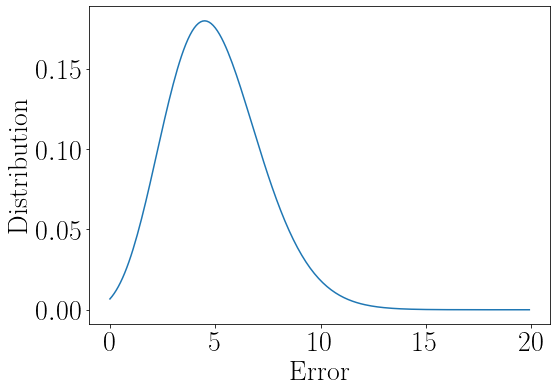
\includegraphics[width=\linewidth]{./img/poisson_distribution.png}
    \caption{Distribution far from 0}
    \label{fig:poisson}
  \end{subfigure}
  \hfill
  \begin{subfigure}{0.47\textwidth}
    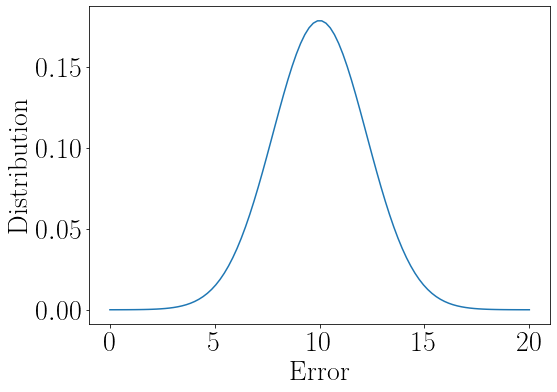
\includegraphics[width=\linewidth]{./img/normal_distribution.png}
    \caption{Distribution close to 0}
    \label{fig:normal}
  \end{subfigure}
  \hfill
  \caption{Two possible error distributions, the left one is more consistently close to zero and is thus better as an error of zero is desired.}
  \label{fig:example_distributions}
\end{figure}

Since, for reproducibility purposes, each model shall generate a distribution of error metrics one cannot any longer compare algorithms based on single metric values. Figure \ref{fig:example_distributions}, presents two examples of possible error distributions. Since a smaller error is generally considered better, it makes sense that distributions concentrated close to zero perform the best. For example, an algorithm generating an error distribution like in Figure \ref{fig:poisson}, is more likely to produce errors close to 0 than an algorithm producing the error distribution in Figure \ref{fig:normal}.

In summary to perform accurate comparisons:
\begin{enumerate}
  \item Suitable error metrics should be used for the domain and datasets.
  \item The distribution of the error metric over multiple runs shall be used when comparing different algorithms.
\end{enumerate}

\chapter{Designing a Benchmarking System}
\label{cha:designing}
A benchmarking system for benchmarking of forecasting methods should fullfill the requirements defined in Chapter \ref{cha:approach}. These requirements, summarized in Table \ref{tab:requirements_summary}, require further specification. For example; which encapsulation system should be used, what is a suitable hypothesis test for statistical reproducibility, how should distributions of errors be compared and how should a representable subset of datasets be chosen. This chapter answers these questions and presents a benchmarking architecture which enables fair, accurate and reproducible comparisons of forecasting algorithms.

\begin{table}[h]
  \begin{tabular}{rc|ccccc}
    Requirement                          &
    \#                                   &
    \rothalf{Accurate}                   &
    \rothalf{Fair}                       &
    \rothalf{Technically reproducible}   &
    \rothalf{Statistically reproducible} &
    \rothalf{Conceptually reproducible}                          \\
    \hline
    Multiple error metrics available     & 1 & X &   &   &   &   \\
    Compare distributions of errors      & 2 & X & X & X & X & X \\
    Optimally tuned models               & 3 &   & X & X &   &   \\
    Multiple datasets used               & 4 &   & X &   &   & X \\
    Public datasets used                 & 5 &   &   & X &   & X \\
    Reference code for ML models         & 6 &   & X & X &   &   \\
    Use encapsulation tools              & 7 &   & X & X &   &   \\
    Use statistical tests                & 8 &   &   &   & X &   \\
    \hline
  \end{tabular}
  \caption{Requirements of a fair, accurate and reproducible benchmarks.}
  \label{tab:requirements_summary}
\end{table}

\section{Design Considerations}
\label{sec:design_considerations}
This section investigates how different tools and techniques can be combined into a benchmarking system for performing fair, accurate and reproducible comparisons of foreasting methods as per the requirements presented in Table \ref{tab:requirements_summary}.

Due to the popularity of Docker and its native capability to encapsulate code and dependencies, Docker containers are chosen as the encapsulation tool for this project. An advantage with docker containers is that popular tools such as Github, AWS, Azure and Dockerhub allows for storage and sharing of Docker images which makes it trivial for researchers to distribute their algorithms in a ready to use package.

Docker containers are however not sufficient for complete technical reproducibility as arguments can be passed to the containers when training commences. For example, the docker image for Gluon-TS allows hyperparameters and the degree of multithreading to use to be specified as arguments. If any such arguments are not detailed when presenting these algorithms in, e.g., a research paper, technical reproducibility becomes hard to achieve. The Runtool described in Section \ref{subsec:runtool} simplifies these things as the config file used when running the experiment can be used by a third party to rerun exactly the same experiment as long as the Docker image and dataset is available.

Reference implementations of complex algorithms are required for fair comparisons, Gluon-TS which was presented in Section \ref{subsec:gluonts_overview} offers several algorithms ranging from simple naive solutions to highly complex DNN hybrid models. Furthermore, Gluon-TS offers ready to use Dockerfiles for both CPU and GPU execution of these algorithms. An additional benefit of leveraging Gluon-TS is that multiple datasets are available for training and testing algorithms on and that multiple error metrics are calculated as part of their backtesting system.

As per the discussion in Section \ref{sec:fair_comparisons}, a fair and conceptually reproducible comparison should make use of multiple datasets with different complementary characteristics. Gluon-TS offers several datasets used in research papers and competitions, and an analysis of these needs to be performed to identify a representable subset. Such an analysis is performed in Section \ref{sec:dataset_analysis}. Furthermore, since the datasets in Gluon-TS are public, rule 5 from Table \ref{tab:requirements_summary} is fullfilled.

In order to capture distributions of error metrics, the seed of the encapsulated algorithms should not be set from within the Docker image otherwise distributions of error metrics would not be generated. This would violate the requirement from Section, requirement 2 from Table \ref{tab:requirements_summary} would be violated as each run would be deterministic.

Since two sample hypothesis tests can be used for the purpose of verifying wether two distributions of error metrics are sampled from the same underlying distribution this type of statistical test is chosen to enforce rule 8 of Table \ref{tab:requirements_summary}. Three hypothesis tests for comparing distributions for reproducibility purposes were discussed in Section \ref{sec:hypothesis_tests}. However the practical performance of such tests when applied to real world distributions of error metrics need to be examined. Particularly, the amount of data needed for them to be accurate needs to be determined so that suitably large distributions of error metrics are collected when benchmarking. In Section \ref{sec:compairing_hypothesis_tests}, such an analysis is performed.

It is common for benchmarks and competitions to generate tables where different forecasting models are compared using real valued numbers to describe their performance. Normally this number is an error metric \cite{m3_competition,makridakis_m4_2020,m5,hyndman_forecasting_3rd,salinas_deepar_2019,oreshkin_n_beats_2020}. Similarly, it would be suitable if a real number could be used to summarize the distribution of error metrics. The conversion from a distribution to a single number is unlikely to be lossless, however it is important that the conversion should accurately represent the distribution by benefiting errors close to 0 and punishing errors further away. Such a conversion should not be limited by the error metric used in the distribution but be applicable to any error metric otherwise requirement 1 in Table \ref{tab:requirements_summary} would be violated.

Tuning of algorithms is a requirement for fair comparisons, thus the possibility of hyperparameter tuning should also be available as part of the benchmarking suite. Since many ML models exhibit non-deterministic behaviour, each hyperparameter configuration being tested should be executed multiple times and aggregated, otherwise rule 2 from Figure \ref{tab:requirements_summary} would be violated.

To summarize, Docker images are chosen to be the encapsulation tool. Further, the Runtool will be used to execute the images as it makes backtests technically reproducible per design. Furthermore, the datasets and forecasting algorithms available in Gluon-TS will be used for the benchmark as these are publicly available and the models are well tested reference implementations. Hyperparameter optimization should be applied to algorithms to enable fair comparisons, and for models with non-deterministic output, each configuration should be executed multiple times when tuning. Benchmarks shall be executed multiple times to collect a distribution of error metrics and a suitable aggregation method for ranking error distributions is needed. In order for benchmarks to be statistically reproducible two error distributions from the same algorithm on the same dataset and with the same hyperparameters should pass a two sample hypothesis test.

\section{Proposed Benchmarking System}
This section introduces a benchmarking system based on the design consideration in Section \ref{sec:design_considerations}.
In Figure \ref{fig:proposed_benchmarking_system}, an overview of the proposed benchmarking system is displayed. Here the benchmark starts by a user providing the Runtool configuration file containing the algorithm to use, the name of the image to use and other data such as which hyperparameters to pass to the algorithm. The system then downloads the datasets identified in Section \ref{sec:dataset_analysis} to the local machine for later use.

\begin{figure}[h]
  \centering
  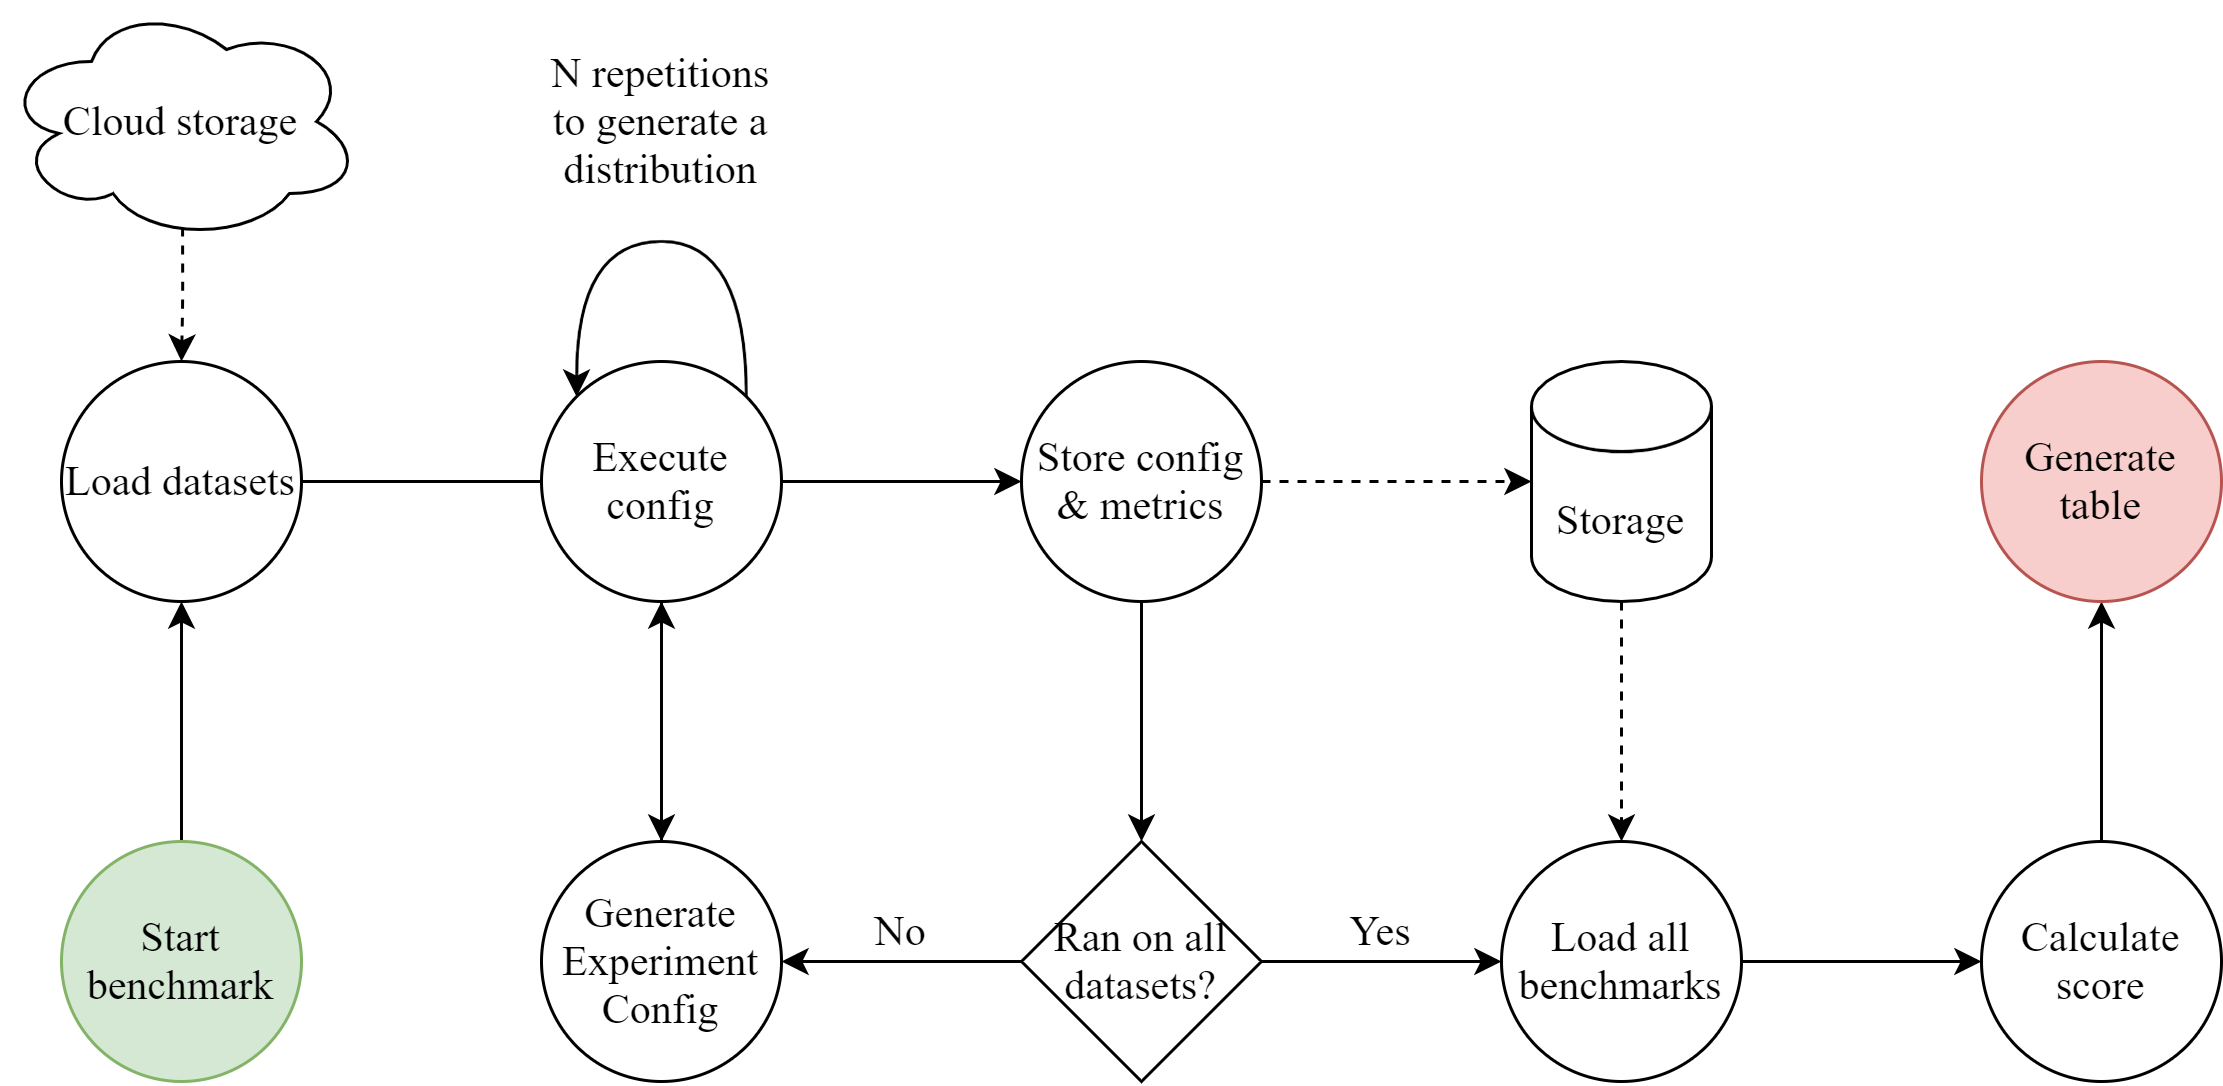
\includegraphics[width=\linewidth]{./img/benchmarking_system_architecture.png}
  \caption{Proposed benchmarking system.}
  \label{fig:proposed_benchmarking_system}
\end{figure}

The benchmarking loop is as follows: the algorithm configuration file is first loaded into the Runtool and an experiment is generated where the algorithm is executed on each of the datasets \textit{N} times. The value of \textit{N} is determined in Section \ref{sec:compairing_hypothesis_tests}. Each time the algorithm is executed, error metrics are reported by the Gluon-TS Backtesting functionality and these logs are captured by the Runtool and stored to a file or database for long term storage. This file will be referred to as the \textit{Benchmark Result File} (BRF) for the remainder of the thesis. Along with the distribution of error metrics, the config file used should be stored in the BRF to make it possible to rerun each benchmark.

The latest benchmarks error distribution is then aggregated through some scoring method which summarizes the distribution as a single value. This is then repeated for each previous benchmark which has been run. The resulting scores are then used to rank the algorithms against each other. A table is then presented to the user showing the relative rank of the latest benchmark compared to the previous benchmarks.

\section{Reproducing Benchmarks}
\label{sec:reproduce_benchmarks}
\begin{figure}[h]
  \centering
  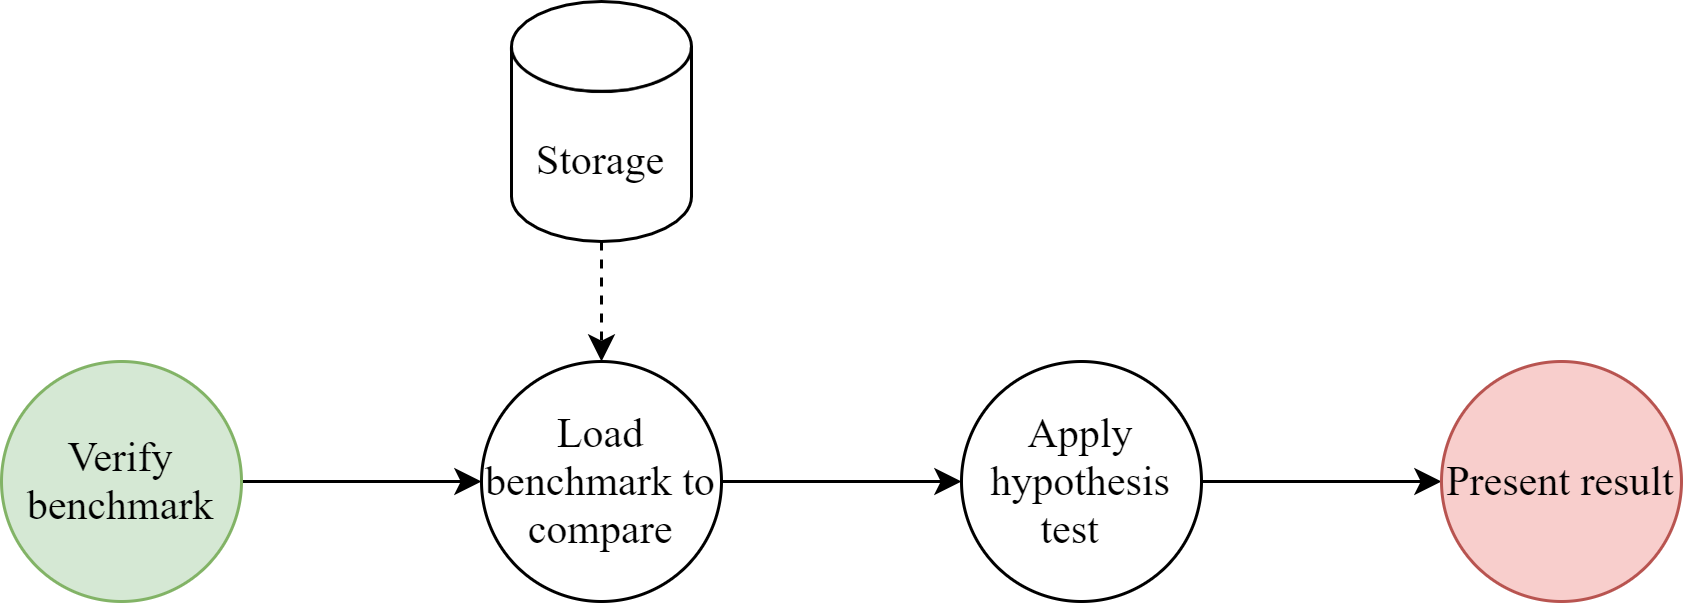
\includegraphics[width=\linewidth]{./img/verify_benchmark.png}
  \caption{Proposed system for verifying benchmarks.}
  \label{fig:proposed_validation_system}
\end{figure}
This section introduces a verification system which can assert statistical reproducibility to benchmarks, an overview over it can be seen in Figure \ref{fig:proposed_validation_system}.
In order to both technically and statistically be able to reproduce a benchmark, a user would need access to the image used and the BRF created by the benchmarking system. Provided these, the verification system could rerun the benchmark using the config file stored in the BRF and the provided image. Rerunning a benchmark with the same setup should result in a similar distribution being generated by the algorithm. Statistically speaking, if the algorithm in the image would be the same as the reference algorithm, both error metric distributions would be sampled from the same underlying distribution. The new distribution can then be compared with that of the benchmark stored in the BRF through a suitable hypothesis test.


\section{Hyperparameter Tuning}
\label{sec:hpo}
\begin{figure}[h]
  \centering
  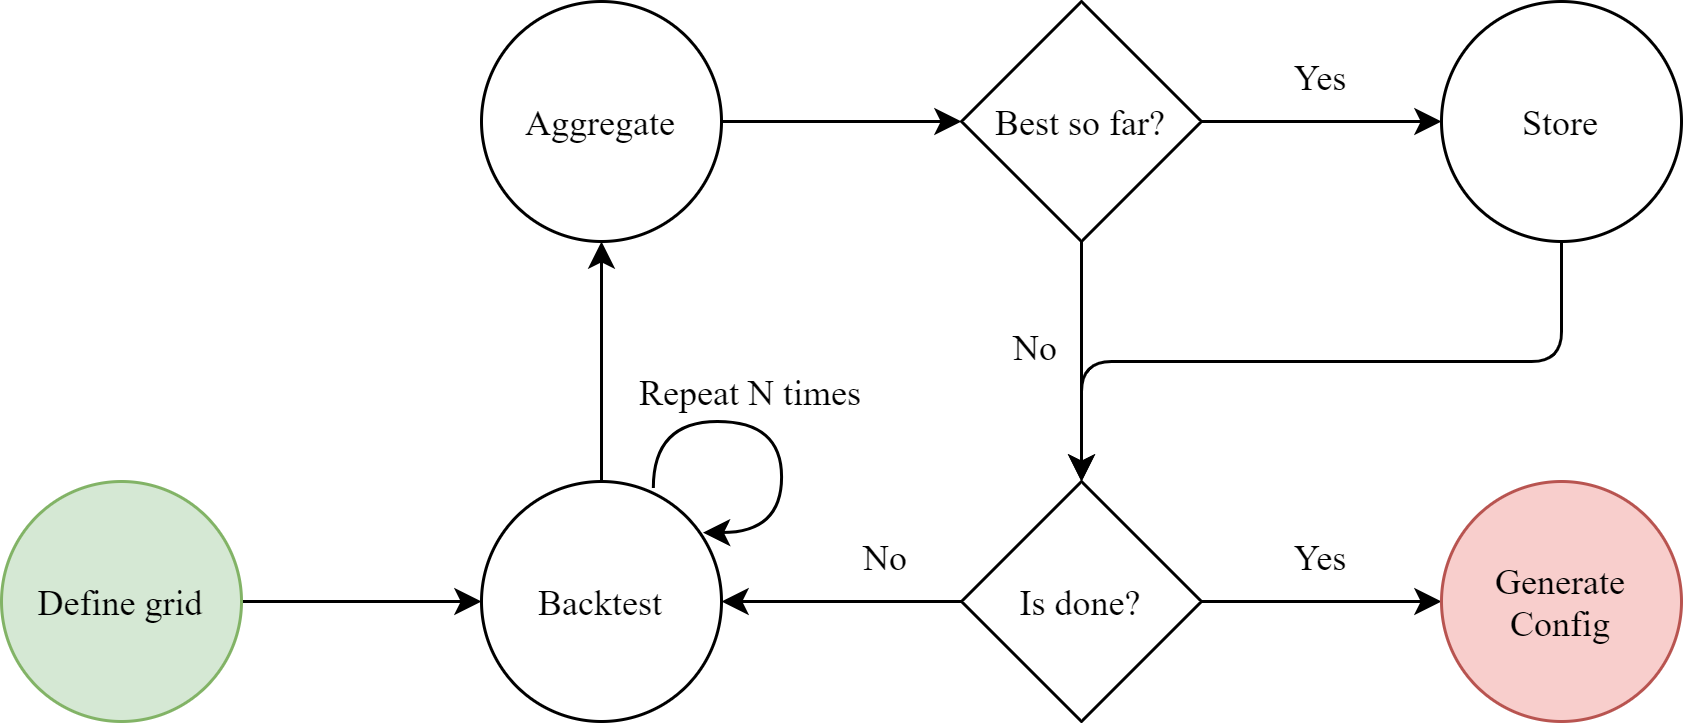
\includegraphics[width=\linewidth]{./img/tuning_overview.png}
  \caption{Proposed system for hyperparameter optimization with repeated runs.}
  \label{fig:proposed_hyperparameter_tuning}
\end{figure}
Hyperparameter tuning is a non-trivial task in itself and many advanced solutions exist such as Bayesian hyperparameter search, hyperband search or advanced meta learning approaches \cite{snoek2012practical,feurer2019hyperparameter, li2017hyperband}. The hyperparameter tuning approach proposed here is not intended to supersede these. Instead it focuses on taking the non deterministic output of each run into account when tuning. Figure \ref{fig:proposed_hyperparameter_tuning}, presents an overview of the proposed hyperparameter tuning system.

The proposed tuning system is in essence a simple grid search tuning algorithm with one major difference. Each configuration in the tuning loop is executed multiple times and then aggregated before being evaluated. Common ML frameworks which offer grid search such as SageMaker or SciKit-Learn (sklearn) surprisingly lack the capability to backtest each configuration multiple times \cite{sagemaker_website, scikit-learn}. While sklearn does offer a cross validation version of its grid search implementation, \textit{GridSearchCV}, this splits the dataset into multiple parts for each iteration. Thus it does not serve the same purpose as performing the backtest multiple times and aggregating the results.

Grid search was chosen as the tuning approach for this system as it is conceptually simple and it is a well known method. It does however have the downside that many unfavorable hyperparameter configurations are evaluated, something which e.g. bayesian search avoids \cite{snoek2012practical}.

An issue with the suggested tuning architecture is that time for tuning increases linearly with the number of repeated runs. Due to this, it may be suitable in real life scenarios to apply this approach as a second step after a set of promising hyperparameter configurations has been identified by another more time efficient approach.

\section{Dataset Analysis}
\label{sec:dataset_analysis}
It is common that new forecasting methods are compared on several datasets as to showcase their predictive power in different scenarios. Different datasets exhibit different characteristics such as trend and seasonality. By identifying a representable set of datasets with complementary characteristics, one can evaluate how robust a forecasting algorithm is to different datasets. Choosing a representable subset of datasets is also needed as the time to train an algorithm scales with the amount of datasets that it should be trained on. For an empirical comparison such as this, it is unfeasible to run training and tuning jobs for all algorithms and datasets available in Gluon-TS since this would take too long. In the remainder of this section an analysis of the datasets available in Gluon-TS is performed to identify a representable subset with diverse characteristics.

\subsection{Methodology}

For each dataset in Gluon-TS plots of the average time series along with one standard deviation from it is generated. This is done to get an overview of what the datasets looks like. Plotting time series for this purpose is common practice in time series forecasting, or as Hyndaman et al. so eloquently put in Forecasting: Principles and practice: \textit{"The first thing to do in any data analysis task is to plot the data."} \cite{hyndman_forecasting_3rd}.

\begin{figure}[htb]
  \centering
  \begin{subfigure}{0.49\textwidth}
    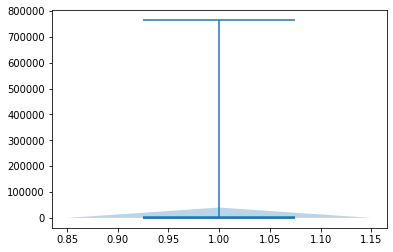
\includegraphics[width=\linewidth]{./img/electricity_violin_unscaled.png}
    \caption{Unscaled violin plot}
    \label{fig:electricity_violin_unscaled}
  \end{subfigure}
  \hfill
  \begin{subfigure}{0.49\textwidth}
    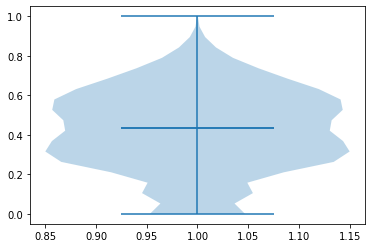
\includegraphics[width=\linewidth]{./img/electricity_violin.png}
    \caption{Scaled violin plot.}
    \label{fig:electricity_violin_scaled}
  \end{subfigure}
  \hfill
  \caption{Violin plots of the Electricity dataset with and without scaling.}
\end{figure}

% \begin{figure}[htb]
%   \centering
%   \minipage{0.5\textwidth}
%   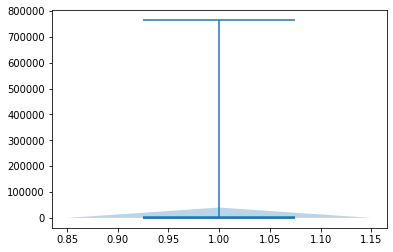
\includegraphics[width=\linewidth]{./img/electricity_violin_unscaled.png}
%   \caption{Unscaled violin plot}
%   \label{fig:electricity_violin_unscaled}
%   \endminipage\hfill
%   \minipage{0.5\textwidth}
%   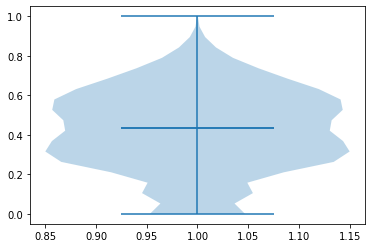
\includegraphics[width=\linewidth]{./img/electricity_violin.png}
%   \caption{Scaled violin plot}
%   \label{fig:electricity_violin_scaled}
%   \endminipage\hfill
%   \caption{Violin plots of the Electricity dataset with and without scaling.}
% \end{figure}

A common tool for visualising time series is to generate a histogram of the time series data. However as the datasets available in Gluon-TS contains tens of thousands of time series, plotting each of these individually is unfeasible. Instead the average time series and one standard deviation of its values is plotted. Another common method for visualizing single time series is to generate a histogram of its values \cite{hyndman_forecasting_3rd}. Instead of generating such histograms violin plots are used in as these capture both the distribution of values just as histograms do as well as the median value and the interquartile range. Since each time series is on its own scale, the aggregate violin plots are hard to read as seen in Figure \ref{fig:electricity_violin_unscaled}. By scaling each time series in the dataset by the maximum value of that time series before plotting it the violin plot becomes easier to interpret, see Figure \ref{fig:electricity_violin_scaled}.

In addition to the visual tools the following statistics is calculated for each of the datasets in Gluon-TS:

\begin{itemize}
  \item Mean value
  \item Max value
  \item Min value
  \item Number of time series
  \item Number of datapoints
  \item Length of shortest time series
  \item Length of longest time series
  \item Strength of the trend (mean and standard deviation)
  \item Strength of the seasonality (mean and standard deviation)
\end{itemize}

Simple metrics such as the maximum, mean and minimum values provide a high level overview of the dataset and helps identifying possible issues which can surface further down the line. For example, the MAPE metric is unstable for time series close to zero as a division with zero occurs \cite{goodwin_asymmetry_1999}.

The number of time series are important for global models as these then have more data which they can learn across which help to combat overfitting. However, the number of time series is not important for local models as these are only impacted by the quality and length of each individual time series. Longer time series however, benefit forecasting models which can handle longer horizons \cite{makridakis_m4_2020}.

For these reasons, the number of time series and the lengths of the shortest and longest time series are necessary metrics when comparing datasets. Optimally one would have both long time series and many series as this would benefit both global and local models.

K-fold cross validation as discussed in Section \ref{sec:evaluating_performance} is a method for increasing the number of series in a dataset. Most of the datasets in Gluon-TS have had K-fold cross validation applied to them already. Thus the potential size after applying K-fold cross validation should be considered for those datasets for which it has not yet been applied.

In Chapter \ref{cha:chapter2}, it was shown that the strength of seasonality (SoS) and the strength of the trend (SoT) of time series are useful metrics for differentiating time series. Due to this, these two measures are the main criterias by which the datasets are chosen. Since each dataset can have both a SoT and SoS, the most diverse datasets are those with complimentary SoT and SoS. In total four datasets can then be identified which fullfill these criteria; one with both high SoT and high SoS, one with high SoT and low SoS, one with low SoT and high SoS and one with both low SoT and low SoS. Since each time series within a dataset is unlikely to have the same SoT or SoS also the variance of the SoT and SoS need to be taken into account. Thus, when two datasets have similar strength, the one with the lowest variance is chosen. This emphasizes the diversity of the datasets as two datasets with high variance in SoS or SoT are prone to contain more similar time series having similar SoT and SoS.

Since larger datasets make models less prone to overfit, the largest dataset is chosen in case of a tie where two datasets are exhibiting a negligible difference in SoT and SoA. Table \ref{dataset_criteria} presents the criterias used for identifying a representable subset of datasets.

\begin{table}[h]
  \begin{tabular}{cc}
    \# & Criteria                                         \\
    1  & One dataset with high trend and low seasonality  \\
    2  & One dataset with low trend and high seasonality  \\
    3  & One dataset with low trend and low seasonality   \\
    4  & One dataset with high trend and high seasonality \\
    5  & Lower variance of strengths is prefered          \\
    6  & Larger dataset chosen in case of a tie           \\
  \end{tabular}
  \caption{Criteria for identifying a representable subset of datasets.}
  \label{dataset_criteria}
\end{table}


\subsubsection{Limitations}
The M4 dataset does not significantly differ to the M3 dataset except for its size \cite{m3_vs_M4}. Thus, the M3 dataset is not considered in this comparison. Another set of datasets which are not going to be used are the NIPS datasets. This is due to them having had postprocessing applied to them. As the exact post processing is not known, comparing any findings when training on these datasets with other papers becomes hard and introduces uncertainty.

\subsection{Result}
To calculate the strengths of the trend and seasonality, a STL decomposition is needed for each time series in the dataset. This decomposition is done using the STL method of the Statsmodel package in Python \cite{seabold2010statsmodels}. The SoS is then calculated using Equation \ref{eq:strength_of_seasonality} and the SoT is calculated using Equation \ref{eq:strength_of_trend}. To summarize the strengths, the mean value and the standard deviation is then calculated of the SoS \& SoT for each dataset.

The complete plots and statistics are available in the appendix as they were to numerous to be displayed here. However a summary of the extracted statistics is presented in Table \ref{tab:dataset_statistics}.


\begin{table}[h]
  \pgfplotstabletypeset[
    color cells={min=0,max=1},
    col sep=comma,
    columns/Dataset/.style={reset styles,string type},
    /pgfplots/colormap={whiteblue}{rgb255(0cm)=(255,255,255); rgb255(1cm)=(2,138,4)},
    /pgf/number format/.cd,
    fixed,
    fixed zerofill,
    precision=2,
  ]{
    Dataset,Trend,Seasonality,Trend Dev., Seasonality Dev.
    Exchange Rate,1,0.12,0,0.3
    M4 Daily, 0.98,0.05,0.05,0.1
    M4 Yearly,0.93,0.09,0.13,0.16
    M4 Quarterly,0.9,0.2,0.16,0.27
    M4 Monthly, 0.84,0.32,0.32,0.3
    M4 Weekly,0.77,0.31,0.31,0.35
    Electricity,0.65,0.84,0.17,0.19
    M4 Hourly,0.62,0.88,0.37,0.16
    Wiki Rolling, 0.53,0.23,0.27,0.26
    M5,0.38,0.28,0.32,0.33
    Traffic,0.16,0.67,0.12,0.1
    Solar Energy, 0.09,0.84,0.03,0.02
    Taxi,0.02,0.66,0.02,0.08
  }
  \caption{Strength of trend \& seasonality for datasets in Gluon-TS.}
  \label{heatmap_strengths}
\end{table}

There is only one dataset in Table \ref{heatmap_strengths} which exhibits low trend and low seasonality and that is the M5 dataset. However the M5 dataset does show the most variance of all the datasets which implies that it contains many time series with and without trend and seasonality. Despite this, since it is the largest dataset available and that there are no other datasets which exhibit low average trend \& seasonality, the M5 dataset is deemed appropriate for use in the benchmarking system.

\clearpage
\begin{table}[htb]
  \begin{tabular}{c | c c c c c c c c c}
    \rothalf{Dataset} & \rothalf{Mean} & \rothalf{Series} & \rothalf{Items} & \rothalf{Shortest} & \rothalf{Longest} & \rothalf{Min} & \rothalf{Max} & \rothalf{Freq.} \\ [0.5ex]
    \hline
    Elec.             & 2510.68        & 321              & 6755124         & 21044              & 21044             & 0.0           & 764000.0      & 1H              \\
    Elec.             & 2509.92        & 2247             & 47501580        & 21068              & 21212             & 0.0           & 764000.0      & 1H              \\
    \hline
    Exch.             & 0.68           & 8                & 48568           & 6071               & 6071              & 0.01          & 2.11          & 1B              \\
    Exch.             & 0.68           & 40               & 246440          & 6101               & 6221              & 0.01          & 2.11          & 1B              \\
    \hline
    Solar             & 40.35          & 137              & 960233          & 7009               & 7009              & 0.0           & 509.05        & 10min           \\
    Solar             & 40.25          & 959              & 6813695         & 7033               & 7177              & 0.0           & 509.05        & 10min           \\
    \hline
    Traf.             & 0.06           & 862              & 12099032        & 14036              & 14036             & 0.0           & 0.72          & H               \\
    Traf.             & 0.06           & 6034             & 85272488        & 14060              & 14204             & 0.0           & 0.72          & H               \\
    \hline
    Exch.*            & 0.68           & 8                & 48568           & 6071               & 6071              & 0.01          & 2.11          & B               \\
    Exch.*            & 0.68           & 40               & 246440          & 6101               & 6221              & 0.01          & 2.11          & B               \\
    \hline
    Elec.*            & 607.95         & 370              & 2142282         & 1081               & 5833              & 0.0           & 168100.0      & H               \\
    Elec.*            & 652.36         & 2590             & 10340239        & 1105               & 4000              & 0.0           & 168100.0      & H               \\
    \hline
    Solar*            & 40.35          & 137              & 960233          & 7009               & 7009              & 0.00          & 509.05        & H               \\
    Solar*            & 40.25          & 959              & 6813695         & 7033               & 7177              & 0.00          & 509.05        & H               \\
    \hline
    Traf.*            & 0.05           & 963              & 3852963         & 4001               & 4001              & 0.00          & 1.00          & H               \\
    Traf.*            & 0.05           & 6741             & 26964000        & 4000               & 4000              & 0.00          & 1.00          & H               \\
    \hline
    Wiki              & 3720.54        & 9535             & 7551720         & 792                & 792               & 0.00          & 7752515.00    & D               \\
    Wiki              & 3663.55        & 47675            & 40619100        & 792                & 912               & 0.00          & 7752515.00    & D               \\
    \hline
    Taxi              & 8.79           & 1214             & 1806432         & 1488               & 1488              & 0.0           & 265.0         & 30min           \\
    Taxi              & 7.41           & 67984            & 54999056        & 149                & 1469              & 0.0           & 225.0         & 30min           \\
    % \hline
    % M3 Mo.            & 4928.47        & 1428             & 141858          & 48                 & 126               & 80.00         & 86730.00      & M                   \\
    % M3 Mo.            & 4971.28        & 1428             & 167562          & 66                 & 144               & -1200.00      & 86730.00      & M                   \\
    % \hline
    % M3 Q              & 4819.27        & 756              & 30956           & 16                 & 64                & 126.00        & 20245.00      & 3M                  \\
    % M3 Q              & 4983.53        & 756              & 37004           & 24                 & 72                & 121.00        & 20375.00      & 3M                  \\
    % \hline
    % M3 Y              & 4417.05        & 645              & 14449           & 14                 & 41                & 30.00         & 39666.22      & 12M                 \\
    % M3 Y              & 4815.77        & 645              & 18319           & 20                 & 47                & 30.00         & 45525.66      & 12M                 \\
    % \hline
    % M3 O              & 6152.18        & 174              & 11933           & 63                 & 96                & 28.00         & 59472.00                            \\
    % M3 O              & 5999.87        & 174              & 13325           & 71                 & 104               & 28.00         & 59472.00                            \\
    \hline
    M4 H              & 6827.69        & 414              & 353500          & 700                & 960               & 10.00         & 703008.00     & H               \\
    M4 H              & 6859.56        & 414              & 373372          & 748                & 1008              & 10.00         & 703008.00     & H               \\
    \hline
    M4 D              & 4951.40        & 4227             & 9964658         & 93                 & 9919              & 15.00         & 352000.00     & D               \\
    M4 D              & 4960.15        & 4227             & 10023836        & 107                & 9933              & 15.00         & 352000.00     & D               \\
    \hline
    M4 W              & 3738.52        & 359              & 366912          & 80                 & 2597              & 104.69        & 51410.00      & W               \\
    M4 W              & 3755.97        & 359              & 371579          & 93                 & 2610              & 104.69        & 51410.00      & W               \\
    \hline
    M4 M              & 4193.28        & 48000            & 10382411        & 42                 & 2794              & 20.00         & 132731.31     & M               \\
    M4 M              & 4207.51        & 48000            & 11246411        & 60                 & 2812              & 20.00         & 177950.00     & M               \\
    \hline
    M4 Q              & 4141.00        & 24000            & 2214108         & 16                 & 866               & 19.50         & 82210.70      & 3M              \\
    M4 Q              & 4287.13        & 24000            & 2406108         & 24                 & 874               & 19.50         & 82210.70      & 3M              \\
    \hline
    M4 Y              & 3630.52        & 23000            & 715065          & 13                 & 300               & 22.10         & 115642.00     & 12M             \\
    M4 Y              & 4076.24        & 23000            & 852909          & 19                 & 300               & 22.00         & 158430.00     & 12M             \\
    \hline
    M5                & 1.12           & 30490            & 57473650        & 1885               & 1885              & 0.00          & 763.00        & D               \\
    M5                & 1.13           & 30490            & 58327370        & 1913               & 1913              & 0.00          & 763.00        & D               \\
    \hline
  \end{tabular}
  \caption{Statistics of the datasets, top row for each dataset is the train split, the bottom row is the test split.}
  \label{tab:dataset_statistics}
\end{table}
\clearpage

In order to choose a dataset which fits into the category of high seasonality and low trend there are three options; Solar Energy, Taxi and Traffic. Of these the Solar Energy dataset has the lowest variance for both the trend and the seasonality. This in addition to having the second lowest average trend of the three and \(23\)\% higher average seasonality than the Taxi and the Traffic datasets makes it most suitable according to the criteria in Table \ref{dataset_criteria}.

The datasets with the lowest seasonality and the highest trends are the M4 datasets except for the M4 Hourly as well as the Exchange rate dataset. The one with the lowest variance and the highest trend of these is the Exchange Rate dataset closely followed by the M4 Daily dataset. The M4 Daily has lower variance for both strength and seasonality, and Table \ref{tab:dataset_statistics} shows that the size of the Exchange Rate dataset is only 8 time series and 48k datapoints in comparison to the 4227 series and 9.9M datapoints the M4 Daily dataset. Thus the M4 Daily is more suited than the Exchange Rate dataset as a representable dataset. Furthermore, all other M4 datasets exhibit a higher variance than the M4 Daily which enforces the M4 Daily to be a better choice for this comparison.

When it comes to finding a dataset which exhibit both high trend and a high seasonality, there are only two options, the Electricity dataset and the M4 Hourly dataset. They both have a high variance, however the variance of the Electricity dataset is slightly lower than that of M4 Hourly. In addition, the Electricity dataset has almost twice the amount of datapoints as M4 Hourly. Thus the Electricity dataset is chosen as it fits the criteria better.

% \begin{figure}[htb]
%   \centering
%   \minipage{0.48\textwidth}
%   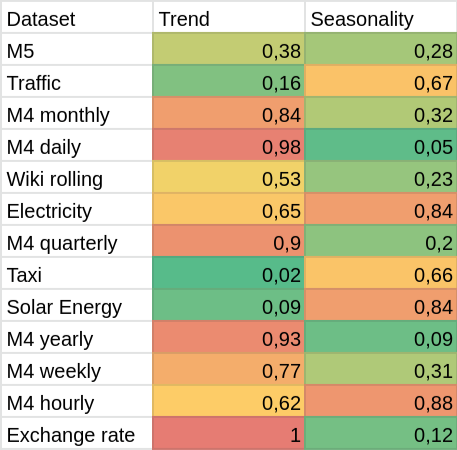
\includegraphics[width=\linewidth]{./img/dataset_trend_seasonality_heatmap_mean.png}
%   \caption{Heatmap of the strength of the trend and the seasonality sorted by the size of the datasets.}
%   \endminipage\hfill
%   \minipage{0.48\textwidth}
%   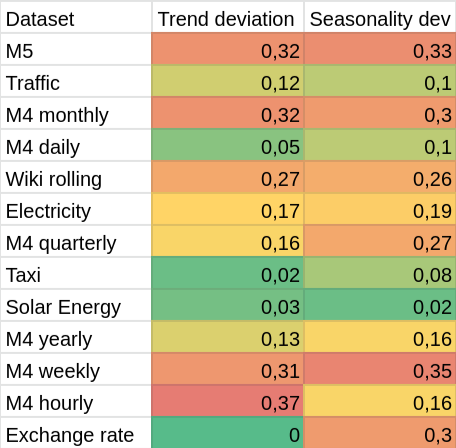
\includegraphics[width=\linewidth]{./img/dataset_trend_seasonality_heatmap_deviation.png}
%   \caption{Heatmap of the standard deviation of the strength of the trend and the seasonality for the datasets.}
%   \endminipage\hfill
% \end{figure}  

To summarize the four datasets which most closely fit the criteria from Table \ref{dataset_criteria} are:

\begin{table}[htp]
  \centering
  \begin{tabular}{ccc}
                              & \textbf{Low trend} & \textbf{High Trend} \\
    \hline
    \textbf{Low seasonality}  & M5                 & M4 Daily            \\
    \hline
    \textbf{High Seasonality} & Solar Energy       & Electricity         \\
  \end{tabular}
  \caption{Datasets with complimentary strengths of trend and seasonality}
  \label{fig:representative_subset_of_datasets}
\end{table}

\section{Comparing Tests for Validating Forecasting Performance}
\label{sec:compairing_hypothesis_tests}
This section investigates the performance of three hypothesis tests for use on distributions of error metrics. The investigated tests are the T-test, Welch’s T-Test and the Kolmogorov-Smirnov two sample test.

Gluon-TS catches accuracy regressions through checking whether new forecasts are within \(1.645\) standard deviations, i.e., within the 95th percentile of past values \cite{gluonts-github}. This approach is based on the assumption that the distribution of error metrics is normally distributed. If this is true then, this simpler approach may be more suitable than a hypothesis test for reproducibility. Thus this approach will be evaluated along with the hypothesis tests.

In order to decide which tests are suitable, certain aspects of the tests and the data need to be investigated. Since the naive test and the parametric tests rely on that the distributions are well defined to function it is important to identify how error distributions of forecasting methods look like, i.e., is it normally distributed or do they follow other distributions.

Different tests require different amount of samples to be accurate, and some tests can become unstable if the sample sizes differ too much \cite{hassani2015kolmogorov, student_or_welch}. Since performing a benchmark is time consuming, it is beneficial from a time perspective to collect as few samples as possible. Thus identifying how the tests perform when applied to different sample sizes is important as a minimum sample size can be identified.

A summary of the questions this minor study aim to answer are:

\begin{itemize}
  \item Which test is best for limited data
  \item Is a parametric test suitable or is a non-parametric test needed
  \item What is a reasonable sample size
  \item Which test has the lowest false reject ratio for related distributions
  \item Is a naive standard deviation based test sufficient
\end{itemize}


\subsection{Methodology}
\label{hypothesis_test_methodology}
Several of the questions which need to be answered require distributions of error metrics to be collected. For this purpose, the DeepAREstimator presented in Section \ref{algo:deepar} is suitable as it is both quick to train and a non-trivial forecaster. The dataset chosen is the Electricity dataset since it is a medium to small sized dataset, thus shortening the required training time.

The Runtool is then used to create 900 experiments where the DeepAREstimator is executed on the Electricity dataset. 300 of these runs has the hyperparameter \textit{distr\_output} set to StudentTOutput, 300 runs are executed with \textit{distr\_output} set to use the NegativeBinomialDistribution. The remaining 300 runs are executed using the Poisson distribution. The three distributions generated by these 900 training jobs are referred to as NB, ST and P in this chapter.

After the distributions are collected, histograms of the distributions are created to identify whether the distributions are visually different. This is done since if all three are visually similar it is unlikely that they can be used for evaluating the hypothesis tests. Further, a visual analysis can determine whether the naive method and or the T-test is suitable since it requires normally distributed data.

After the visual analysis, the ratio of false rejects are calculated, i.e., how often the test is unable to detect that two samples are sampled from the same distribution. To answer this questions, let \(N\) be the total distribution and \(X,Y\) be the two samples drawn from \(N\). The size of \(X\) is then defined by \[k \leq |X| \leq |N| - |Y|\] where \(k\) is a constant value. Similarly, the size of \(Y\) varies between: \[k	\leq |Y| \leq |N|-k\] For each sample of \(X\) and \(Y\) the tests are applied and false negatives are recorded.

In order to evaluate a suitable minimum sample size, heatmaps are generated where the tests are applied to the three distributions with varying sample sizes. Each test is performed with a \textit{P value} of 0.05. If the test accepts the samples to be from the same distribution the color green is used while a rejection, is colored red.

\subsection{Results}

\begin{figure}[htb]
  \centering
  \minipage{0.49\textwidth}
  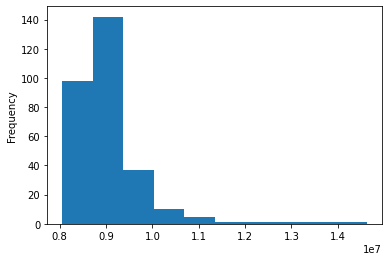
\includegraphics[width=\linewidth]{./img/histogram_deepar_electricity_statistics_300_samples.png}
  \caption{Student-T}
  \label{deepar_student_t_distibution}
  \endminipage\hfill
  \minipage{0.49\textwidth}
  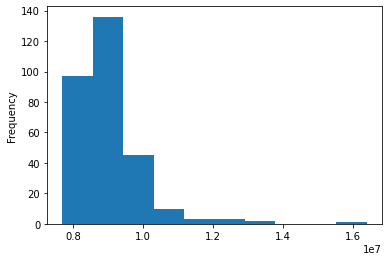
\includegraphics[width=\linewidth]{./img/histogram_deepar_negbin_electricity_statistics_200_samples.png}
  \caption{Neg-Binomial}
  \label{deepar_negbinomial_distibution}
  \endminipage\hfill
  \\
  \minipage{0.49\textwidth}
  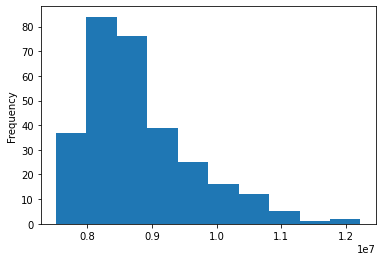
\includegraphics[width=\linewidth]{./img/histogram_deepar_poisson_electricity_statistics_200_samples.png}
  \caption{Poisson}
  \label{deepar_poisson_distribution}
  \endminipage
  \caption{Histograms of the absolute error for 300 runs of DeepAR on the Electricity dataset with three different values of the hyperparameter \emph{distr\_output}}
  \label{deepar_elec_300_hist}
\end{figure}


The histograms shown in Figure \ref{deepar_elec_300_hist} do not resemble a normal distribution. Instead all three histograms are more closely approximating a log normal distribution. Note that the histogram in Figure \ref{deepar_student_t_distibution} and \ref{deepar_negbinomial_distibution} are very similar while the one in Figure \ref{deepar_elec_300_hist} differs. This indicates that different hyperparameter configurations for a single algorithm impacts the error distribution.


\begin{table}[htp]
  \centering
  \begin{tabular}{lcccc}
    {\textbf Name}    & {\textbf \%} & {\textbf configuration} \\
    \hline
    Naive             & $<$1\%       & Negative Binomial       \\
    Naive             & $<$1\%       & Student T               \\
    Naive             & $<$1\%       & Poisson                 \\
    \hline
    T-Test            & 5\%          & Negative Binomial       \\
    T-Test            & 5\%          & Student T               \\
    T-Test            & 32\%         & Poisson                 \\
    \hline
    Welchs T-Test     & 11\%         & Negative Binomial       \\
    Welchs T-Test     & 8\%          & Student T               \\
    Welchs T-Test     & 31\%         & Poisson                 \\
    \hline
    Kolmogorv-Smirnov & 3\%          & Negative Binomial       \\
    Kolmogorv-Smirnov & 5\%          & Student T               \\
    Kolmogorv-Smirnov & 21\%         & Poisson                 \\
    \hline
  \end{tabular}
  \caption{Number of times when the algorithm failed to recognize that the samples were from the same distribution}
  \label{tab:false_rejects}
\end{table}

In Table \ref{tab:false_rejects} the amount of false rejections of the three hypothesis tests and the naive solution is presented. From this data it is clear that the Naive solution is the best performing with a 1\% chance of failing to validate that the two samples are from the same distribution. The Kolmogorov-Smirnov performs second best, however it is incorrect 21\% of the time when evaluating on the distribution generated by the Poisson configuration. The two T-Tests are the worst performers, performing worse than or equal to the Kolmogorov-Smirnov test on all distributions.

Since the distributions of error metrics are not reminiscent of the normal distribution, the naive method, the T-test and the Welch's T-test which are parametric tests are unsuitable for use when verifying dataset distributions. The data in Table \ref{tab:false_rejects} further enforces this since Kolmogorov-Smirnov is the second best performer for all distributions where only the naive method is better. In Figure \ref{naive_negative_bin_poisson} the naive method is evaluated on the Poisson and Negative Binomial distributions. It is clear from this heatmap that the naive method is prone to accept quite different distributions for all but small sample sizes. This behaviour is also apparent on all other heatmaps where the naive method is used, see Appendix \ref{app:naive_heatmaps}. This is expected since the distributions all have similar average values even though their distributions are visually different. In comparison, the Kolmogorov-Smirnov test is able to differentiate all distributions given sufficient sample sizes, see Figures \ref{ks_student_t_poisson}, \ref{ks_student_t_neg_bin}, \ref{ks_neg_bin_poisson}.

The sample size required to differentiate between different distributions (true negatives) as well as the sample sizes required for true positives for the Kolmogorov-Smirnov test is presented in Table \ref{tab:required_sample_sizes}. This table summarizes the heatmaps generated for the Kolmogorov-Smirnov test when applied to samples of varying sizes from the three distributions as described in \ref{hypothesis_test_methodology}. Additional heatmaps not shown in this chapter are available in Appendix \ref{app:heatmaps}.


\begin{table}[htp]
  \centering
  \begin{tabular}{cccc}
                      & Student T & Poisson & Negative Binomial \\
    \hline
    Student T         & \(>50\)   &         &                   \\
    \hline
    Poisson           & \(>25\)   & \(>45\) &                   \\
    \hline
    Negative Binomial & \(>160\)  & \(>60\) & \(<130\)          \\
  \end{tabular}
  \caption{Required sample sizes for the Kolmogorov Smirnov test on three distributions of error metrics.}
  \label{tab:required_sample_sizes}
\end{table}

\begin{figure}[h]
  \centering
  \minipage{0.7\textwidth}
  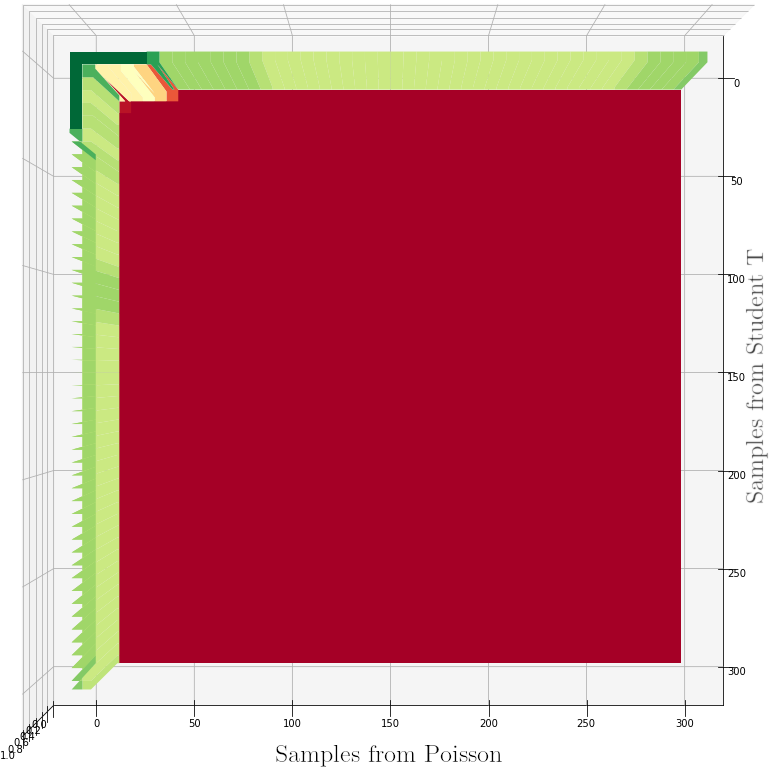
\includegraphics[width=\linewidth]{./img/hypothesis_test/deepar_heatmap_Y_student_t_X_poisson_ks_edited.png}
  \endminipage
  \caption{Heatmap of KS applied to the ST and P distributions.}
  \label{ks_student_t_poisson}
\end{figure}
\clearpage

From Table \ref{tab:required_sample_sizes} it is shown that the KS test becomes accurate for true positives at a sample size of at least 40 samples. However, it seems as if KS can become unstable for sample sizes above 130. To be able to use the KS statistic to distinguish between different distributions, sample sizes above 160 may be needed if the distributions are visually very similar, otherwise, sample sizes above \(60\) suffice. These values are aligned with the findings of the simulation study performed by Hassani et al. \cite{hassani2015kolmogorov}. There they showed the need for \(>128\) samples to achieve \(>99\)\% rejection rate for similarly looking distributions.

\begin{figure}[h]
  \centering
  \minipage{0.7\textwidth}
  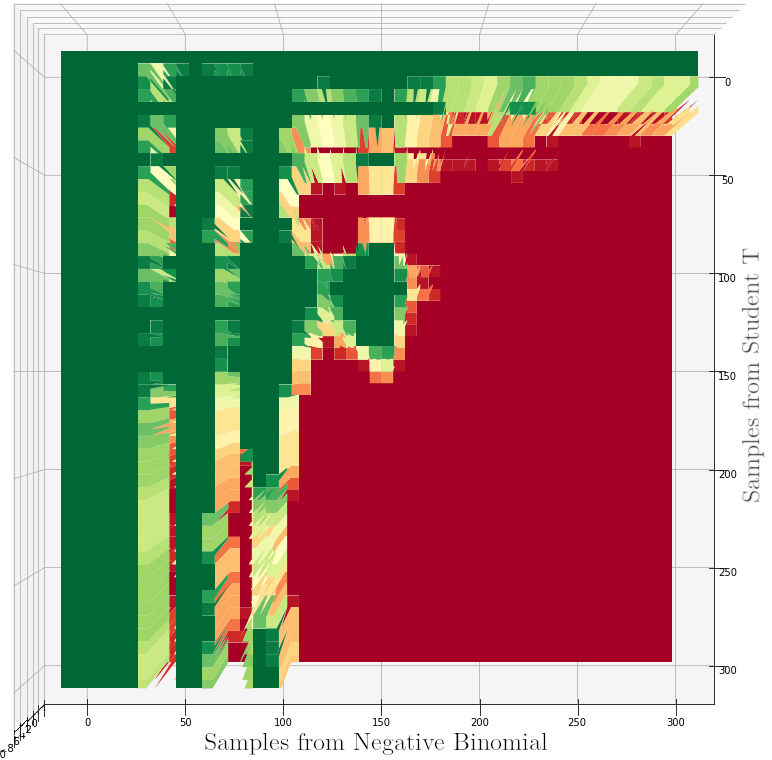
\includegraphics[width=\linewidth]{./img/hypothesis_test/deepar_heatmap_Y_student_t_X_neg_bin_ks_edited.png}
  \caption{Heatmap of KS applied to the ST and NB distributions.}
  \label{ks_student_t_neg_bin}
  \endminipage
\end{figure}

To summarize, despite the limited data available for this comparison, the Naive test, the T-test and Welch’s T-Test has been shown to be unsuitable for comparing distributions of time series forecasting errors due to non-normality of the data. This makes the Kolmogorov-Smirnov two sample test the best suited statistical test for asserting the statistical reproducibility of error metric distributions. When evaluating the Kolmogorov-Smirnov on samples from three different distributions it was shown that \(>60\) samples are required to verify distributions but more than \(160\) may be required to differentiate similar distributions.

\begin{figure}[h]
  \centering
  \minipage{0.65\textwidth}
  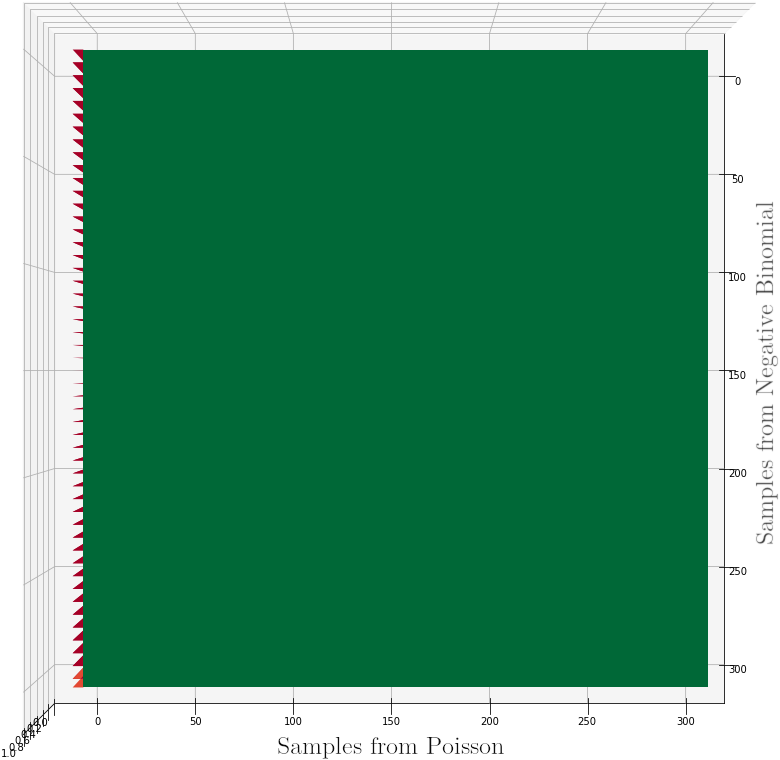
\includegraphics[width=\linewidth]{./img/hypothesis_test/deepar_X_poisson_Y_neg_bin_naive_edited.png}
  \caption{Heatmap of the Naive method applied to the NB and P distributions.}
  \label{naive_negative_bin_poisson}
  \endminipage
  \\
  \minipage{0.65\textwidth}
  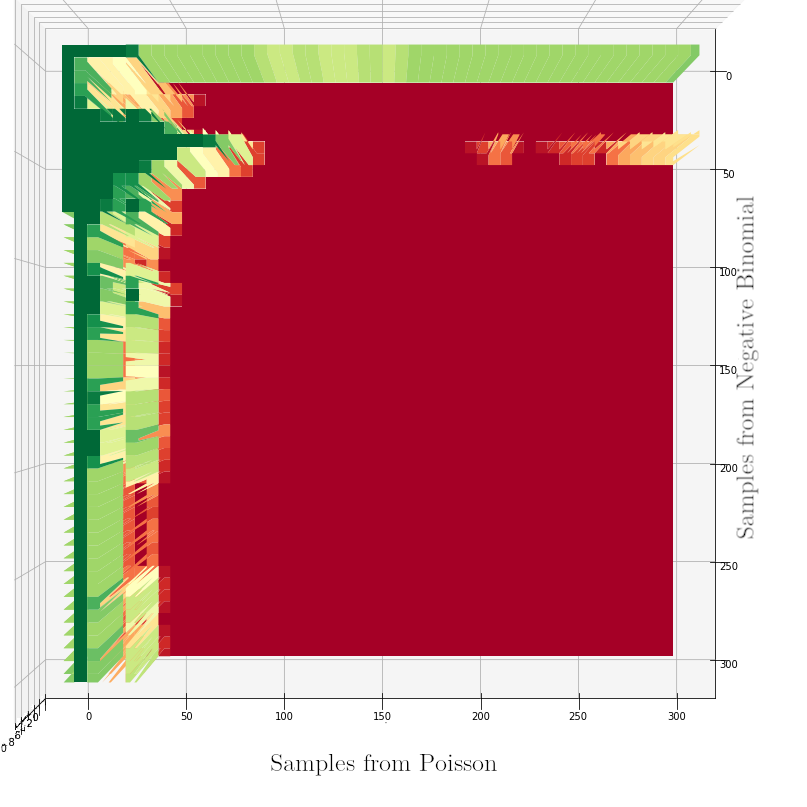
\includegraphics[width=\linewidth]{./img/hypothesis_test/deepar_heatmap_Y_neg_bin_X_poisson_ks_edited_labels.png}
  \caption{Heatmap of KS applied to the NB and P distributions.}
  \label{ks_neg_bin_poisson}
  \endminipage
\end{figure}
\clearpage

\section{Ranking Distributions}
\label{sec:ranking_distributions}
To rank algorithms based on distributions of error metrics, a suitable metric need to be calculated. Since perfect forecasts would result in an error of zero, algorithms where the distributions are close to 0 should recieve a better score than those further away. In Figure \ref{fig:error_metric_distributions} six possible error distributions are shown. Only non-negative distributions are considered here as many common error metrics such as; MAE, RMSE, MSE, MASE, MAPE are non-negative metrics \cite{gluonts-github,hyndman_forecasting_3rd}. Furthermore, a distribution with negative values can converted to a non-negative distributions by taking the absolute value of each element in it.

An optimal ranking of the error distributions in Figure \ref{fig:error_metric_distributions} would favor those most often close to 0 and punish those with heavy tails away from zero. In addition to this a score should favor consistency, i.e., low variance, thus multimodal distributions with one peak close to zero and one further away should perform worse than distribution with a single peak in between.

A metric which fits these criteria in the realm of time series forecasting is the Root Mean Squared Error which was presented in Section \ref{sec:RMSE}. The equation for RMSE is:

\begin{figure}[h]
  \[RMSE = \sqrt{mean((Y - \hat{Y})^2)}\]
  \caption{Equation for calculating RMSE}
\end{figure}

Through fixing the value of the target value \(Y\) to 0 and viewing each datapoint in the error distribution as a forecast \(\hat{Y}\) this metric can be used to aggregate distributions of error metrics where the optimal value is 0. This modified version of RMSE is referred to as RMSE4D (RMSE for Distributions) for the remainder of the thesis.

\begin{figure}[h]
  \[RMSE4D = \sqrt{mean(\hat{Y}^2)}\]
  \caption{Equation for calculating RMSE4D}
\end{figure}

A RMSE4D close to 0 is considered optimal and it is a non-negative error, thus, when comparing two RMSE4D values, lower values are better. An issue with RMSE is that the \(\hat{Y}^2\) part of the equation makes it sensitive to outliers in the data. Thus when calculating the RMSE4D the top 5\% and the bottom 5\% should be removed to account for this.

\subsection{Evaluation of RMSE4D}
To evaluate whether RMSE4D is suitable for aggregating distributions of error metrics, it is evaluated against two simple aggregation techniques, the mean and the median values. These methods are evaluated on six samples of 100 datapoints taken from the distributions shown in Figure \ref{fig:error_metric_distributions}. These six distributions were designed to be as different as possible to identify potential issues with the three aggregation methods.

Histograms of the samples used for the evaluation are shown in Figure \ref{fig:error_metric_distributions_hist}. All of these distributions except for the Exponential in Fig. \ref{exponential_hist} are generated by randomly sampling 100 samples from one or more normal distributions. For brevity a normal distribution with mean $\mu$, and deviation $\sigma$ is written as \(N(\mu,\sigma)\). If two different distributions are combined then 50 samples are taken from each distribution and the combination is expressed as \(N(\mu_1,\sigma_1) + N(\mu_2,\sigma_2)\). Furthermore for all distributions in Figure \ref{fig:error_metric_distributions_hist} the absolute value has been taken of the 100 random samples of the distributions since only non-negative errors are considered.

An optimal ranking of the 6 distributions would be the Exponential in first place since all errors are distributed close to 0. The N(2,2) distribution should be ranked second since no other distribution are close to 0. In third place the N(5,2) distribution in Figure \ref{n_5_2_hist} or the Heavy tailed distribution in Figure \ref{heavy_tailed_distributions_hist} fits since consistent performance is preferred, but the peak of the heavy tailed distribution is closer to 0 than the peak of the N(5,2) distribution. For fifth place the bimodal distribution in Figure \ref{bimodal_distribution_hist} fits since it is more accurate than the N(8,2) distribution. This leaves the N(8,2) distribution for last place.

\begin{table}[htp]
  \centering
  \begin{tabular}{ccccc}
    Distribution                     & RMSE4D   & Mean     & Median   & Optimal rank \\
    \hline
    Exponential                      & 1.15 (1) & 0.88 (1) & 0.72 (1) & 1            \\
    \hline
    N(2,2)                           & 2.55 (2) & 2.10 (2) & 1.96 (3) & 2            \\
    \hline
    Heavy Tailed \(N(0,2) + N(3,5)\) & 4.30 (3) & 2.67 (3) & 1.59 (2) & 3-4          \\
    \hline
    N(5,2)                           & 5.48 (4) & 5.14 (5) & 5.31 (5) & 3-4          \\
    \hline
    Bimodal \(N(1.5,1) + N(8.5,1)\)  & 6.22 (5) & 5.04 (4) & 4.93 (4) & 5            \\ % not median or mean since consistency is prefered
    \hline
    N(8,2)                           & 8.20 (6) & 7.93 (6) & 7.82 (6) & 6            \\
    \hline
  \end{tabular}
  \caption{Values and relative ranks of different aggregation methods for distributions of error metrics.}
  \label{tab:evaluation_crayon_score}
\end{table}

From Table \ref{tab:evaluation_crayon_score} it is clear that the ranking based on the RMSE4D values closely resemble the optimal ranking for the considered distributions. It is shown from these results that heavy tails are punished more by the RMSE4D than by the mean or median which is expected. This can be seen when comparing the methods for the \textit{Heavy Tailed} and \textit{Bimodal} as the accumulate error is much higher for RMSE4D than that of the mean or median. The median method is the least consistent with what is considered the optimal ranking for this scenario and is thus rejected for use when comparing distributions. The mean does generate rankings aligned with the optimal ranking however it fails to favor consistency since it favors the \textit{Bimodal} distribution over the N(5,2) distributions. This indicates that the mean is not suitable to use when aggregating distributions of error metrics as low variance of errors should be encouraged. A benefit of the mean and median however is that the scale of the metric remains the same while the RMSE4D can blow up when large errors are squared. Despite this, the comparison of the three aggregation methods shows that the RMSE4D metric is the superior choice for ranking distributions of error metrics as it favors consistency of error metrics which the mean and the median do not.

\begin{figure}[ht]
  \begin{minipage}[b]{0.5\linewidth}
    \centering
    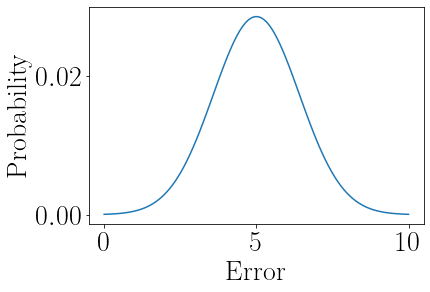
\includegraphics[width=\linewidth]{./img/distributions/normal.png}
    \caption{Gaussian}
    \vspace{4ex}
    \label{n_5_2_hist}
  \end{minipage}%%
  \begin{minipage}[b]{0.5\linewidth}
    \centering
    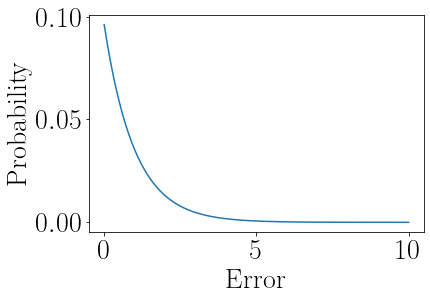
\includegraphics[width=\linewidth]{./img/distributions/exponential.png}
    \caption{Exponential}
    \vspace{4ex}
  \end{minipage}
  \begin{minipage}[b]{0.5\linewidth}
    \centering
    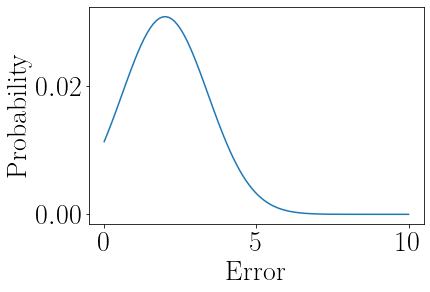
\includegraphics[width=\linewidth]{./img/distributions/normal_n_2_2.png}
    \caption{Normal N(2,2)}
    \vspace{4ex}
    \label{n_2_2_hist}
  \end{minipage}%% 
  \begin{minipage}[b]{0.5\linewidth}
    \centering
    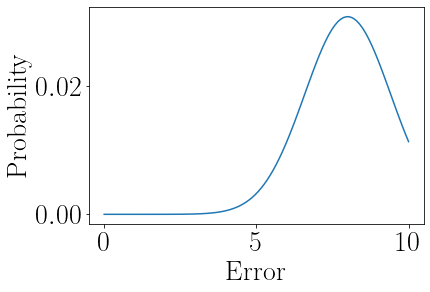
\includegraphics[width=\linewidth]{./img/distributions/normal_n_8_2.png}
    \caption{Normal N(8,2)}
    \vspace{4ex}
  \end{minipage}
  \begin{minipage}[b]{0.5\linewidth}
    \centering
    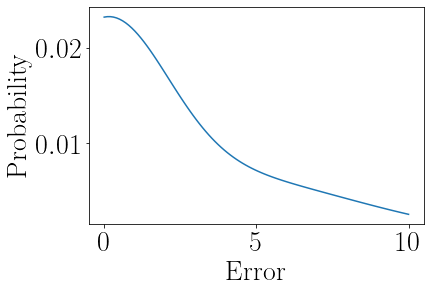
\includegraphics[width=\linewidth]{./img/distributions/heavy_tailed_2.png}
    \caption{Heavy Tailed}
    \vspace{4ex}
    \label{heavy_tailed_distributions}
  \end{minipage}%% 
  \begin{minipage}[b]{0.5\linewidth}
    \centering
    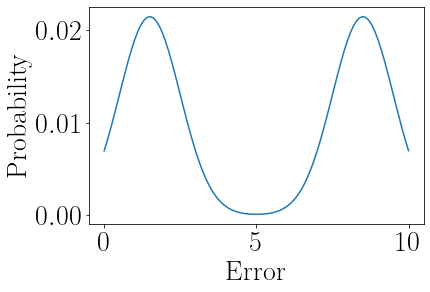
\includegraphics[width=\linewidth]{./img/distributions/twin_peaks.png}
    \caption{Bimodal}
    \label{bimodal_distribution}
    \vspace{4ex}
  \end{minipage}
  \caption{Six possible error metric distributions.}
  \label{fig:error_metric_distributions}
\end{figure}
\begin{figure}[ht]
  \begin{minipage}[b]{0.5\linewidth}
    \centering
    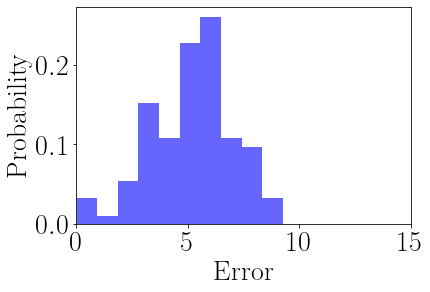
\includegraphics[width=\linewidth]{./img/distributions/normal_hist.png}
    \caption{Normal N(5,2)}
    \vspace{4ex}
  \end{minipage}%%
  \begin{minipage}[b]{0.5\linewidth}
    \centering
    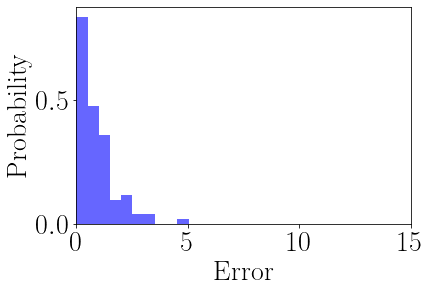
\includegraphics[width=\linewidth]{./img/distributions/exponential_hist.png}
    \caption{Exponential}
    \vspace{4ex}
    \label{exponential_hist}
  \end{minipage}
  \begin{minipage}[b]{0.5\linewidth}
    \centering
    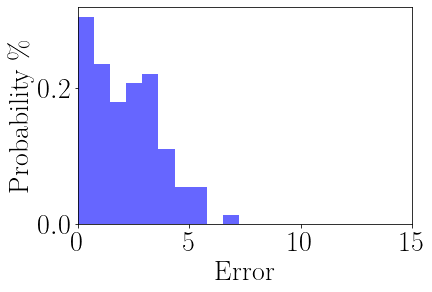
\includegraphics[width=\linewidth]{./img/distributions/normal_n_2_2_hist.png}
    \caption{Normal N(2,2)}
    \vspace{4ex}
  \end{minipage}%% 
  \begin{minipage}[b]{0.5\linewidth}
    \centering
    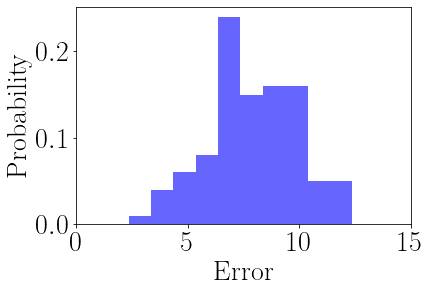
\includegraphics[width=\linewidth]{./img/distributions/normal_n_8_2_hist.png}
    \caption{Normal N(8,2)}
    \vspace{4ex}
  \end{minipage}
  \begin{minipage}[b]{0.5\linewidth}
    \centering
    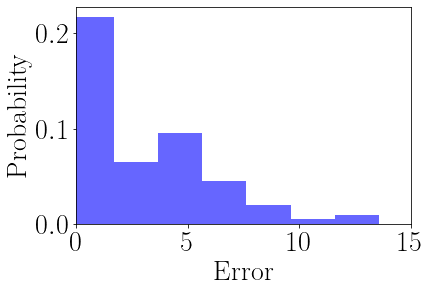
\includegraphics[width=\linewidth]{./img/distributions/heavy_tailed_2_hist.png}
    \caption{Heavy Tailed}
    \vspace{4ex}
    \label{heavy_tailed_distributions_hist}
  \end{minipage}%% 
  \begin{minipage}[b]{0.5\linewidth}
    \centering
    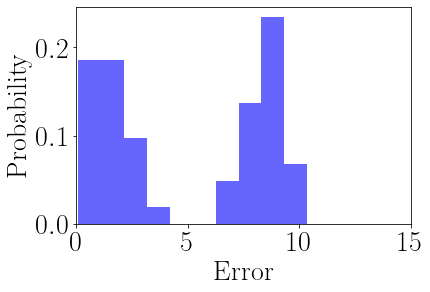
\includegraphics[width=\linewidth]{./img/distributions/twin_peaks_hist.png}
    \caption{Bimodal}
    \label{bimodal_distribution_hist}
    \vspace{4ex}
  \end{minipage}
  \caption{Six histograms from 100 samples of possible error metric distributions.}
  \label{fig:error_metric_distributions_hist}
\end{figure}
% \begin{figure}[htb]
%   \centering
%   \minipage{0.40\textwidth}
%   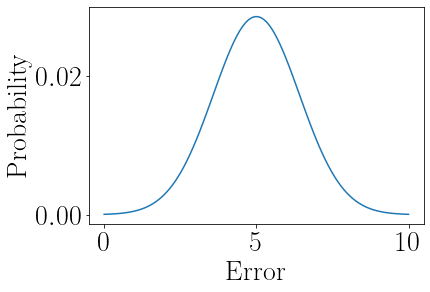
\includegraphics[width=\linewidth]{./img/distributions/normal.png}
%   \caption{Gaussian}
%   \endminipage

%   \minipage{0.40\textwidth}
%   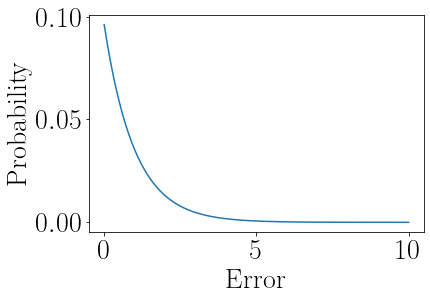
\includegraphics[width=\linewidth]{./img/distributions/exponential.png}
%   \caption{Exponential}
%   \endminipage
%   \\
%   \minipage{0.40\textwidth}
%   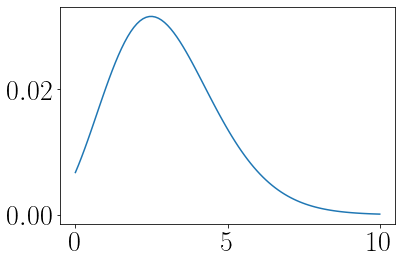
\includegraphics[width=\linewidth]{./img/distributions/poisson.png}
%   \caption{Poisson}
%   \endminipage

%   \minipage{0.48\textwidth}
%   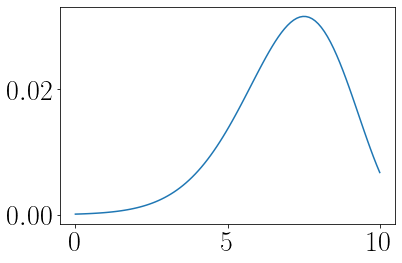
\includegraphics[width=\linewidth]{./img/distributions/reverse_poisson.png}
%   \caption{Reverse Poisson}
%   \endminipage
%   \caption{Different possible distributions of error metrics, which one is best?}
% \end{figure}
\chapter{Crayon}
\label{cha:crayon}

In this section Crayon, a Python toolkit for benchmarking ML forecasting models, is introduced. Crayon contains a set of tools for making fair, accurate and reproducible comparisons between forecasting models. Crayon is open sourced and available on GitHub under the MIT license \cite{crayon_github}.

Crayon is based on the benchmarking architecture presented in Figure \ref{fig:proposed_benchmarking_system}. Technically reproducible results are made through the use of three core technologies; Runtool configuration files for defining reproducible training jobs, Docker images containing the algorithm to benchmark and the public datasets available through Gluon-TS. In order to make benchmarks statistically reproducible error metrics generated from benchmarks can be automatically compared through the Kolmogorov-Smirnov 2 sample hypothesis test. Crayon is error metric agnostic, meaning that any error metrics required for a certain domain can be used, thus enabling accurate comparisons between models. Additionally, a custom error metric for comparing distributions named the Crayon score is implemented. This metric is based on the RMSE metric for time series forecasts and encourages algorithms with low variance in errors.

Since it is common that machine learning workloads are executed in the cloud, as well as locally, both options are supported by Crayon. Since the runtool only supports executing training jobs in AWS SageMaker a custom backend is implemented for local execution.

\section{Algorithms}
\label{crayon:algorithms}
In crayon, the \textit{Algorithms} class contains all the information needed in order to execute an algorithm contained in a Docker image stored either on AWS ECR or on the local machine. \textit{Algorithm} objects are the basic building blocks for performing hyperparameter tuning and for creating runtool configuration files.

An \textit{Algorithm} object contains information about the \textit{image} to run, the \textit{hyperparameters} to use. If the algorithm should be executed on SageMaker, the specific instance it should be run on can also be set using the \textit{instance} parameter. The \textit{Algorithm} class also optionally accepts a dictionary of regexes to the \textit{metrics} parameter. These regexes are used by SageMaker to extract metrics from an algorithms output. Default regexes for Gluon-TS algorithms are available in the \textit{crayon.utils} module. This parameter is not required when executing locally. In Listing \ref{code:algorithm} an example is shown of how the \textit{Algorithm} class is used.

\begin{figure}[h]
  \begin{lstlisting}[language=Python,label={code:algorithm},caption={Example of the Algorithm class.}]
from crayon import Algorithm
Algorithm(
  name="myalgo", 
  image="my_image", 
  instance="local",
  hyperparameters={...},
  metrics={"abs_error": ... }
)
  \end{lstlisting}
  % \caption{Example of the Algorithm class.}
  % \label{code:algorithm}

\end{figure}
\section{Datasets}
\label{crayon:datasets}
The Crayon \textit{Dataset} class wraps all the data needed to locate a dataset on your local machine or on AWS S3. It only takes two required parameters; the \textit{name} of the dataset \& the \textit{path} to the dataset on locally or on AWS S3.

The \textit{path} is a dict which points to the file location(s) of the dataset. If one has a train, test and validation dataset, the items in the \textit{path} will point to these versions of the dataset. Any \textit{meta} information one wish to provide about the dataset in question can be passed through the \textit{meta} parameter. In \ref{code:dataset} an example of how to use the Dataset class is presented.
\begin{figure}[h]
  \begin{lstlisting}[language=Python, label={code:dataset}, caption={Example of the Dataset class.}]
from crayon import Dataset
Dataset(
  name="electricity",
  path={
    "train": "file:///datasets/electricity/train/data.json",
    "test": "file:///datasets/electricity/test/data.json",
  },
  meta={...}
)
  \end{lstlisting}
\end{figure}
\section{Config Generation}
\label{'subsub:config_generation'}
This section discusses the different tools available in Crayon in order to create runtool compatible config files. These config files are a core part of the Crayon functionality and is used in several internal systems. Thus it is important to understand how these are generated and look like. For further information about how the config files function and additional functionality of them, see the section about the runtool (\ref{subsec:runtool}).

Through providing a \textit{Algorithm} object \& a \textit{Dataset} object to the \textit{generate\_config} function in Crayon, a configuration file compatible with the runtool is generated. The intention of this file is that by providing the config, the image used and the dataset to another person, that person could rerun your experiments with the exact same configuration. Internally Crayon uses the \textit{generate\_config} function in order to create tuning and benchmarking training jobs. See \ref{code:config_generation} for an example.
\begin{figure}
  \begin{lstlisting}[language=Python, label={code:config_generation}, caption={Config generation using Crayon}]
from crayon import Algorithm, Dataset, generate_config

# generate runtool configuration file
config = generate_config(
  Algorithm(
    name="myalgo",
    image="my_image",
    hyperparameters={"epochs": 10},
  ),
  Dataset(
    name="my_ds",
    path={
      "train": "/datasets/electricity/train/data.json",
      "test": "/datasets/electricity/test/data.json",
    },
  ),
  "/Users/freccero/Documents/config.yml",
)
\end{lstlisting}
\end{figure}

After executing the code in \ref{code:config_generation}, a config file is stored to the path provided to \textit{generate\_config}, in this case the config file is stored to \textit{/Users/freccero/Documents/config.yml}. The config file generated by the code in \ref{code:config_generation} is displayed in Listing \ref{code:generated_config}.
\begin{figure}
  \begin{lstlisting}[label={code:generated_config}, caption={Generated configurations file.}]
my_ds:
  meta: {}
  name: my_ds
  path:
    test: file:///datasets/electricity/test/data.json
    train: file://datasets/electricity/train/data.json
myalgo:
  hyperparameters:
    epochs: 10
  image: my_image
  instance: local
  name: myalgo
\end{lstlisting}
\end{figure}


If one does not have a custom dataset but instead wishes to use a reference dataset for training and evaluating the algorithm on, it is possible to use the datasets in Gluon-TS. The \textit{get\_gluonts\_datasets} function downloads any number of Gluon-TS datasets onto the local machine and generates a list of Datasets objects which can be passed to the  \textit{generate\_config} function. Example code for doing so is shown in \ref{code:config_generation_gluonts} with the output of the code displayed in \ref{output:config_generation_gluonts}.

\begin{figure}[h]
  \begin{lstlisting}[language=Python, label={code:config_generation_gluonts}, caption={Config generation using Crayon with gluonts datasets}]
from crayon import Algorithm, Dataset, generate_config, get_gluonts_datasets
import yaml

# generate runtool configuration file
config = generate_config(
  Algorithm(
    name="myalgo",
    image="my_image",
    hyperparameters={"epochs": 10},
  ),
  get_gluonts_datasets(["electricity"]),
  "/Users/freccero/Documents/config.yml",
)

print(yaml.dump(config))
    \end{lstlisting}
\end{figure}
\begin{figure}
  \begin{lstlisting}[label={output:config_generation_gluonts}, caption={Output when executing Code Fragment \ref{code:config_generation_gluonts}}]
electricity:
  meta:
    feat_dynamic_cat: []
    feat_dynamic_real: []
    feat_static_cat:
    - cardinality: '321'
      name: feat_static_cat
    feat_static_real: []
    freq: 1H
    prediction_length: 24
    target: null
  name: electricity
  path:
    test: file:///Users/freccero/.mxnet/gluon-ts/datasets/electricity/test/data.json
    train: file:///Users/freccero/.mxnet/gluon-ts/datasets/electricity/train/data.json
myalgo:
  hyperparameters:
    epochs: 10
  image: my_image
  instance: local
  metrics: null
  name: myalgo
    \end{lstlisting}
\end{figure}





\section{Training}
Given a valid runtool config file Crayon uses this file to start training jobs locally or on AWS SageMaker. The provided config file can be either written by hand or generated using Crayon as described in \ref{'subsub:config_generation'}.

A training job is started by calling the \textit{crayon.run\_config} method with the config. The experiment to run is defined using the mathematical operators + and * as described in section \ref{subsec:runtool}.

The \textit{crayon.run\_config} function returns a \textit{Jobs} object which makes it easy to investigate training results as it stores all metrics reported by the algorithms across all started jobs to a pandas DataFrame.

\subsection{Local Training}
If a config is to be run locally, algorithm defined in the config need to point to an image which is available on the users machine. The image used should be valid for use with AWS SageMaker. Furthermore, any datasets which the algorithm should be trained on should also be available on the local machine. For details of what constitutes a valid SageMaker image, refer to the documentation of SageMaker \cite{sagemaker_docker_documentation}.

In listing \ref{config:local_training} an example configuration file for local training is displayed and in \ref{code:local_training} code for training the algorithm on the dataset in the config is presented.
\begin{figure}[h]
  \begin{lstlisting}[label={config:local_training}, caption={Config file for running local training jobs}]
my_algo:
  image: gluonts:cpu_new
  hyperparameters:
    freq: H
    prediction_length: 24
    forecaster_name: gluonts.model.deepar.DeepAREstimator
  instance: local

my_dataset:
  path:
    train: file:///datasets/electricity/train/data.json
    test: file:///datasets/electricity/test/data.json
  \end{lstlisting}
\end{figure}
\begin{figure}[h]
  \begin{lstlisting}[language=Python, label={code:local_training}, caption={Code for running local training jobs using Crayon}]
from crayon import run_config

jobs = run_config(
  config="config.yml",
  combination="config.my_algo * config.my_dataset",
)
  \end{lstlisting}
\end{figure}


By executing the code in Code Fragment \ref{code:local_training} Crayon will use the runtool to load the config in \ref{config:local_training} and start training jobs locally through the \textit{local\_run} method of the runtool. The jobs will be executed sequentially. After the jobs finish, Crayon looks for a file named \textit{agg\_metrics.json} or \textit{metrics.json} in the output directory for each job. This file is expected to contain any metrics reported by the algorithm being trained. An example json file is shown in \ref{output:local_job_output} for reference.

\begin{figure}
  \begin{lstlisting}[label={output:local_job_output}, caption=Example of a training job output file such as \textit{metrics.json} or \textit{agg\_metrics.json}]
{
  "MSE": 6703174.123610994,
  "abs_error": 37402126.36717987,
  "MASE": 1.62229213532052,
  "MAPE": 0.23736356524438723
}
\end{lstlisting}
\end{figure}


\subsection{Cloud Training}
\label{sec:cloud_training}
Executing training jobs in SageMaker is done similarly as when starting them locally, but with some alterations to the config file and to the python script.

The config file needs to refer to an image available in ECR of the AWS account that is to be used. Further, the \textit{instance} in the config file must match one of the instance types which SageMaker offers. Any metrics which the algorithm outputs during training such as accuracy metrics or similar must have a corresponding regex under the metrics tag in the config file. This regex is used by SageMaker to parse the algorithm output for metrics. The final change to the config which needs to be done for running on SageMaker is that any datasets needs to be stored in an AWS S3 bucket instead of locally.

In addition to the above changes to the config file, three further parameters are required by the \textit{run\_config} function in the Python script.

\begin{enumerate}
  \item \textit{role\_arn} - The AWS IAM Role  which authorizes Crayon to start training jobs on SageMaker.
  \item \textit{bucket} - The AWS S3 bucket where any artifacts of the training job should be stored.
  \item \textit{session} - A \textit{boto3.Session} object which Crayon will use to interact with SageMaker.
\end{enumerate}

The IAM Role requires permissions to start training jobs on sagemaker, pull AWS ECR images, and read/write access to the provided S3 bucket. For information about how to create a IAM Role with the proper permissions as well as an S3 bucket please refer to the AWS documentation for these two services \cite{iam_website,s3_website}.

In Listing \ref{config:cloud_training}, an example configuration file is displayed which can be used to train on AWS SageMaker and in \ref{code:cloud_training} an example python file is presented which given a config dispatches training jobs to SageMaker using the \textit{run\_config} function of Crayon.

\begin{figure}[h]
  \begin{lstlisting}[label={config:cloud_training}, caption={Config file for running training jobs on SageMaker.}]
my_algo:
  image: 012345678901.dkr.ecr.eu-west-1.amazonaws.com/gluonts:2020-11-01
  hyperparameters:
  freq: H
  prediction_length: 24
  forecaster_name: gluonts.model.deepar.DeepAREstimator 
  instance: ml.m5.xlarge 
  metrics:
  abs_error: 'abs_error\): (\d+\.\d+)'

my_dataset:
  path:
  train: s3://gluonts-run-tool/gluon_ts_datasets/constant/train/data.json
  test: s3://gluonts-run-tool/gluon_ts_datasets/constant/test/data.json
      
  \end{lstlisting}
  % \end{figure}
  % \begin{figure}[h]
  \begin{lstlisting}[language=Python, label={code:cloud_training}, caption={Code for running training jobs on AWS SageMaker using Crayon}]
from crayon import run_config
import boto3

jobs = run_config(
  config="config.yml",
  combination="config.my_algo * config.my_dataset",
  role_arn="arn:aws:iam::012345678901:role/service-role/my_role",
  bucket="my_bucket",
  session=boto3.Session(),
)
    \end{lstlisting}

\end{figure}

\section{Tuning}
In order to use Crayon as a benchmarking tool, it is advised that each algorithm has been suitably tuned to the datasets which it should run on. This is required since comparing a finely tuned model with an undertuned model will result in unfair comparisons being made.

Grid search is a common strategy used when tuning algorithm. When tuning using grid search, one creates for each hyperparameter a list of values which that hyperparameter can take. Thereafter the algorithm is then run for each combination of these parameters. The hyperparameter combination resulting in the best results is then returned as the optimal hyperparameter combination to use.

Below I present how an algorithm can be tuned using the grid-search functionality in Crayon.

\subsection{Grid-Search}
Grid search is done using the \textit{grid\_search} function in the \textit{Crayon.Tuner} module. The \textit{grid\_search} function is implemented based on the architecture suggested in \ref{sec:hpo} with some additional features. Since multiple runs of an algorithm generates a small distribution of values, the method used for aggregating these is customizable, per default the mean is taken. Further, since different metrics may optimize towards different values, a custom method for comparing values can be passed, per default lower aggregate errors are better. Each hyperparameter configuration generated by \textit{grid\_search} is stored into a runtool configuration file. This simplifes the benchmarking of a tuned algorithm as the generated runtool config file can be used directly by the \textit{crayon.benchmark} method presented in Section \ref{subsec:benchmarking}.

An overview of the features of the \textit{grid\_search} module is displayed in Figure \ref{features_grid_search}:

\begin{figure}[h]
  \begin{itemize}
    \item Performs grid search with both static and changing parameters.
    \item Each hyperparameter combination can be rerun multiple times to handle non-deterministic algorithms
    \item Allows passing a custom function for aggregating error metrics from jobs.
    \item Allows passing of a custom scoring function for evaluating jobs.
    \item Generates runtool configuration files for each combination of hyperparameters.
  \end{itemize}
  \caption{Features of the grid search functionality in Crayon.}
  \label{features_grid_search}
\end{figure}


\subsubsection{Overview of the grid\_search function in Crayon}
\begin{figure}
  \begin{lstlisting}[language=Python, label={code:grid_search_signature}, caption={Parameters of the grid search functionality in Crayon.}]
def grid_search(
  changing_hyperparameters: dict,
  target_metric: str,
  dataset: Dataset,
  algorithm: Algorithm,
  output_dir: str = crayon_dir().resolve(),
  aggregation_function: Callable = statistics.mean,
  evaluation_function: Callable = lambda new, old: new < old,
  run_locally: bool = True,
  **kwargs,
) -> GridSearchResults:
    \end{lstlisting}
\end{figure}
In Code Fragment \ref{code:grid_search_signature} the signature for the \textit{grid\_search} method of Crayon is displayed. Each of the parameters of this method will here be presented and in Code Fragment \ref{code:grid_search_local} an example of how to perform grid search locally is presented.

In Code Fragment \ref{code:grid_search_signature} \textit{changing\_hyperparameters} are the hyperparameters which are to be tuned. This parameter takes a dictionary where the keys are the hyperparameters to tune and the value is a list of values which they should take. The \textit{target\_metric} parameter selects which metric that the algorithm outputs should be optimized for. Further, the grid search takes a \textit{crayon.Dataset} and a \textit{crayon.Algorithm} (see Sections \ref{crayon:algorithms} \& \ref{crayon:datasets}). Any hyperparameters defined within the \textit{algorithm} stays the same for each run in the training loop. The \textit{output\_dir} determines where the Runtool configuration files created for each hyperparameter combination will be stored.

The \textit{aggregation\_function} is used to merge the results if each configuration should be run more than once. Per default this is done is by taking the mean of the recorded values. Through passing a custom function to the \textit{aggregation\_function} parameter one can override this behaviour. This function needs to take a list of numbers as a parameters and it needs to return a single value. In Code Fragment \ref{code:grid_search_local} the \textit{mean} function is provided from the \textit{statistics} module of pythons standard library.

The \textit{evaluation\_function} is used to determine whether the results of the most recent hyperparameter combination were better than the best seen hyperparameter combination so far. The default behaviour defines that if the new value of the target metric is lower than the best so far, it is better. This makes sense whenever one wishes to minimize the target metric, i.e. an absolute error of 10 is better then an absolute error of 100. However for other target metrics, different behaviour may be more suitable. Providing a function which takes two parameters, the new value and the old value and compares these to the \textit{evaluation\_function} parameter the behaviour is customized. The \textit{run\_locally} parameter determines if the jobs should be executed on the local machine or on AWS SageMaker. Any additional parameters passed is forwarded to the \textit{crayon.run\_config} function for each training job. Thus, for executing in SageMaker the parameters defined in Section \ref{sec:cloud_training} need to be passed in addition.

In Code Fragment \ref{code:grid_search_local} grid search is performed on an image containing gluonts. The algorithm being tuned in Gluon-TS is the DeepAREstimator with the hyperparameters \textit{freq} and \textit{prediction\_length} being the same for each training job. The grid search tries to minimizing the average value of the \textit{abs\_error} metric over two runs for each hyperparameter combination. The hyperparameters that are tuned are the \textit{epochs} and the \textit{context\_length}.
\begin{figure}
  \begin{lstlisting}[language=Python, label={code:grid_search_local}, caption={Grid search running locally.}]
grid_search(
  algorithm=Algorithm(
    name="deepar",
    image="gluonts_cpu",
    hyperparameters={
      "freq": "D",
      "prediction_length": 7,
      "forecaster_name": "gluonts.model.deepar.DeepAREstimator",
    },
  ),
  dataset=Dataset(
    name="electricity",
    path={
      "train": "file:///electricity/train/data.json",
      "test": "file:///electricity/test/data.json",
    },
  ),
  runs=2,
  target_metric="abs_error",
  aggregation_function = statistics.mean, 
  evaluation_function = lambda new, old: new < old,
  changing_hyperparameters={
    "epochs": [1, 5],
    "context_length": [1, 5],
  }
)
  \end{lstlisting}
\end{figure}

% By setting the \textit{run\_locally} parameter to False we tell Crayon to execute the training on SageMaker instead of locally. In order to make this work, we need to provide the an AWS S3 bucket, an AWS IAM role and a boto3 Session object. See section \ref{sec:cloud_training} for more information about these.
% An example of how grid search can be executed on SageMaker is presented in \ref{code:grid_search_cloud}.
% \begin{figure}
%   \begin{lstlisting}[language=Python, label={code:grid_search_cloud}, caption={Grid search running on SageMaker.}]
% from crayon import (
%     GLUONTS_METRICS, Algorithm, Dataset, grid_search
% )
% import boto3

% grid_search(
%   role_arn="arn:aws:iam::012345678901:role/my_role",
%   bucket="my_bucket",
%   run_locally=False,
%   session=boto3.Session(),
%   algorithm=Algorithm(
%     name="deepar",
%     image="my_ecr_url/gluonts/cpu",
%     hyperparameters={
%       "freq": "D",
%       "prediction_length": 7,
%       "forecaster_name": "gluonts.model.deepar.DeepAREstimator",
%     },
%     metrics=GLUONTS_METRICS,
%     instance="ml.m5.xlarge",
%   ),
%   dataset=Dataset(
%     name="electricity",
%     path={
%       "train": "s3://electricity/train/data.json",
%       "test": "s3://electricity/test/data.json",
%     },
%   ),
%   runs=2,
%   target_metric="abs_error",
%   aggregation_function = statistics.mean, 
%   evaluation_function = lambda new, old: new < old,
%   changing_hyperparameters={
%     "epochs": [1, 5],
%     "context_length": [1, 5],
%   }
% )
%     \end{lstlisting}
% \end{figure}
\section{Benchmarking}
\label{subsec:benchmarking}
One of the key components of Crayon is the benchmarking module. This module compares algorithms by backtesting them on four datasets with different characteristics; \textit{M5}, \textit{M4 Daily}, \textit{Electricity} and \textit{Solar Energy}. These datasets were chosen since they exhibit complimentary characteristics as per the discussion in \ref{sec:dataset_analysis}.

To benchmark an algorithm via Crayon a config file describing the algorithm needs to be passed. Furthermore, one must pass which target metric should be the target for the benchmark, i.e. absolute error, MASE, MAPE or any other metric reported by the benchmarked algorithm. Crayon then backtests the algorithm on each dataset 100 times in order to build up a distribution of the target metric. The value 100 was chosen as it is in the middle of the boundraries identified in Section \ref{sec:compairing_hypothesis_tests}. After the error metric distributions have been generated, RMSE4D described in Section \ref{sec:ranking_distributions} is used to compare the errors from the benchmark with previously run benchmarks. A lower value of RMSE4D is better.

As the benchmark is run on multiple datasets, it is important to provide tuned models for each. This is done by appending the dataset name to the algorithm name in the config file so that each algorithm defined in the config file has the structure: \(<algorithm\_name>\_<dataset\_name>\). In Code Fragment \ref{config:benchmarking} an example config file for benchmarking is presented. Note the two hyperparameter configurations of DeepAR in the config, this indicates that different hyperparameters is used for the electricity dataset.

\begin{figure}
  \begin{lstlisting}[language=Python, label={config:benchmarking}, caption={Config file for benchmarking with Crayon. Note that \textit{deepar\_electricity} has a different hyperparameter configuration thus these hyperparameters are used when benchmarking the algorithm on the electricity dataset. For all other datasets, the default algorithm definition \textit{deepar} is used.}]
deepar:
  name: deepar
  image: gluonts:cpu_new
  hyperparameters:
    epochs: 1
    freq:
      $eval: $trial.dataset.meta.freq
    prediction_length:
      $eval: 2 * $trial.dataset.meta.prediction_length
    context_length:
      $eval: 2 * $trial.algorithm.hyperparameters.prediction_length
    forecaster_name: gluonts.model.deepar.DeepAREstimator    
  instance: local

deepar_electricity:
  $from: deepar
  hyperparameters:
    epochs: 2
    \end{lstlisting}

  \begin{lstlisting}[language=Python, label={code:benchmarking}, caption={Python script for starting a benchmarking run using Crayon.}]
from crayon import benchmark

benchmark(
  algorithm_config="config.yml",
  algorithm_name="deepar",
  benchmark_id="my_benchmark",
  target_metric="MASE",
)
    \end{lstlisting}
\end{figure}

After the 100 backtests for each dataset has finished, the recorded error distributions are stored to a file on the local machine. This file also contains the \textit{id} of the benchmark, as well as the config used to create the training jobs. Also the \textit{Jobs} object which was generated from the benchmark are stored into this file. The Jobs objects contain the metrics recorded for a certain Job. The file where these values are stored was referred to as the Benchmark Result File (BRF) in Chapter \ref{cha:designing}. In future versions of Crayon, the BRF could be handled by some centralized storage server instead of locally, however this is out of the scope of the thesis.

\section{Verifying Benchmark Performance}
In \ref{sec:reproduce_benchmarks} an architecture for making benchmarks statistically reproducible was presented. In essence, statistical reproducibility of benchmarks can be made through applying a hypothesis test on the error metric distributions generated by the two benchmarks. Since, in Crayon, each benchmark consists of four distributions of error metrics, one for each dataset, four hypothesis tests need to be performed.

The \textit{Crayon.verify} function in Crayon is based on the architecture proposed in \ref{sec:reproduce_benchmarks}. \textit{Crayon.verify} takes the paths to two BRF files generated by benchmarks. Further, two Benchmark IDs are required in order to identify which benchmarks in the respective files should be verified against each other. The investigation in Section \ref{sec:compairing_hypothesis_tests} concluded that the Kolmogorov Smirnov 2 Sample Test (KS test) is suitable for comparing distributions of error metrics. This test is thus chosen for use in Crayon for verifying benchmarks. Since different metrics are supported by the benchmarking module, the specific metric distribution to verify is required by the \textit{verify} function.

In Code Fragment \ref{code:verify} an example of the \textit{crayon.verify} function is presented. There, two benchmarks from different BRFs are verified against each other using the KS test with respect to the MASE metric. Thus, the KS test is applied to the distributions of the MASE metric for each dataset in turn. If the KS test rejects the two distributions to be samples from the same underlying distribution the algorithms cannot be verified. In Code Fragment \ref{code:outputverification} example output after executing Code Fragment \ref{code:verify} is presented.

\begin{figure}
  \begin{lstlisting}[language=Python, label={code:verify}, caption={Verifying whether two benchmarks are performed by the same algorithm.}]
from crayon import verify

verify(
    id_1="my_benchmark",
    id_1_results_file="BRF_1.yml", 
    id_2="someone_elses_benchmark",
    id_2_results_file="BRF_2.yml",
    target_metric="MASE",
)
\end{lstlisting}
\end{figure}
\begin{figure}
  \begin{lstlisting}[language=bash, label={code:outputverification}, caption={Output from Code Fragment \ref{code:verify}}]
    Algorithm verified on dataset electricity
    Algorithm verified on dataset m4_daily
    Algorithm verified on dataset m5
    Algorithm verified on dataset solar_energy
    Passed 4/4 verifications.
\end{lstlisting}
\end{figure}

\section{Case Study: Preventing Accuracy Regressions in Forecasting Frameworks}
\label{sec:crayon_case_study}
This section investigates how to use the statistical reproducibility which Crayon enable to protect forcasting libraries against accuracy regressions. Specifically, how the \textit{benchmarking} and \textit{verify} functions in Crayon can be used to detect accuracy regression through automated tests. The DeepAREstimator of Gluon-TS will be the focal point of this investigation since it suffered a accuracy regression, which has now been resolved. Thus, distributions can be collected both before, during and after a regression to showcase how these regressions can be detected and how it can be detected when they are resolved.

The DeepAREstimator in Gluon-TS suffered a accuracy regression, between the 7th of May 2020 until 9th of July 2020 for certain values of the \textit{distr\_output} hyperparameter was used. The issue arised due to a change in the way that the \textit{gluonts.distribution.NegativeBinomialOutput} was calculated. The issue was not detected until the 15 June 2020, However, the root cause of the issue was not discovered until the 2nd of July after which the bug was patched within a week on the 9th of July \cite{gluonts_deepar_bugged, gluonts_deepar_bugged_found, gluonts_deepar_patched}. In this case, the time required to detect and resolve the issue was close to two months.

To detect accuracy regression with Crayon, a reference benchmark is required to serve as a ground-truth of the expected performance for an algorithm. When new changes to algorithms or their dependencies happen, a new benchmark should be executed with these changes. These two benchmarks can then be verified using the \textit{crayon.verify} function. If they pass the checks, no accuracy regression has occurred and if the checks failed it indicates that an accuracy regression has occured. When the accuracy regression is fixed a new benchmark can be run as a post-fix benchmark. This post-fix benchmark can be verified towards the ground-truth benchmark to verify if the accuracy is back at the original levels. If a change in accuracy is expected the post-fix benchmark can be used as the new ground-truth for future tests. An overview of this method is shown in Figure \ref{fig:crayon_as_test}. This method is designed to easily be integrated into existing testing workflows.

\begin{figure}[h]
  \centering
  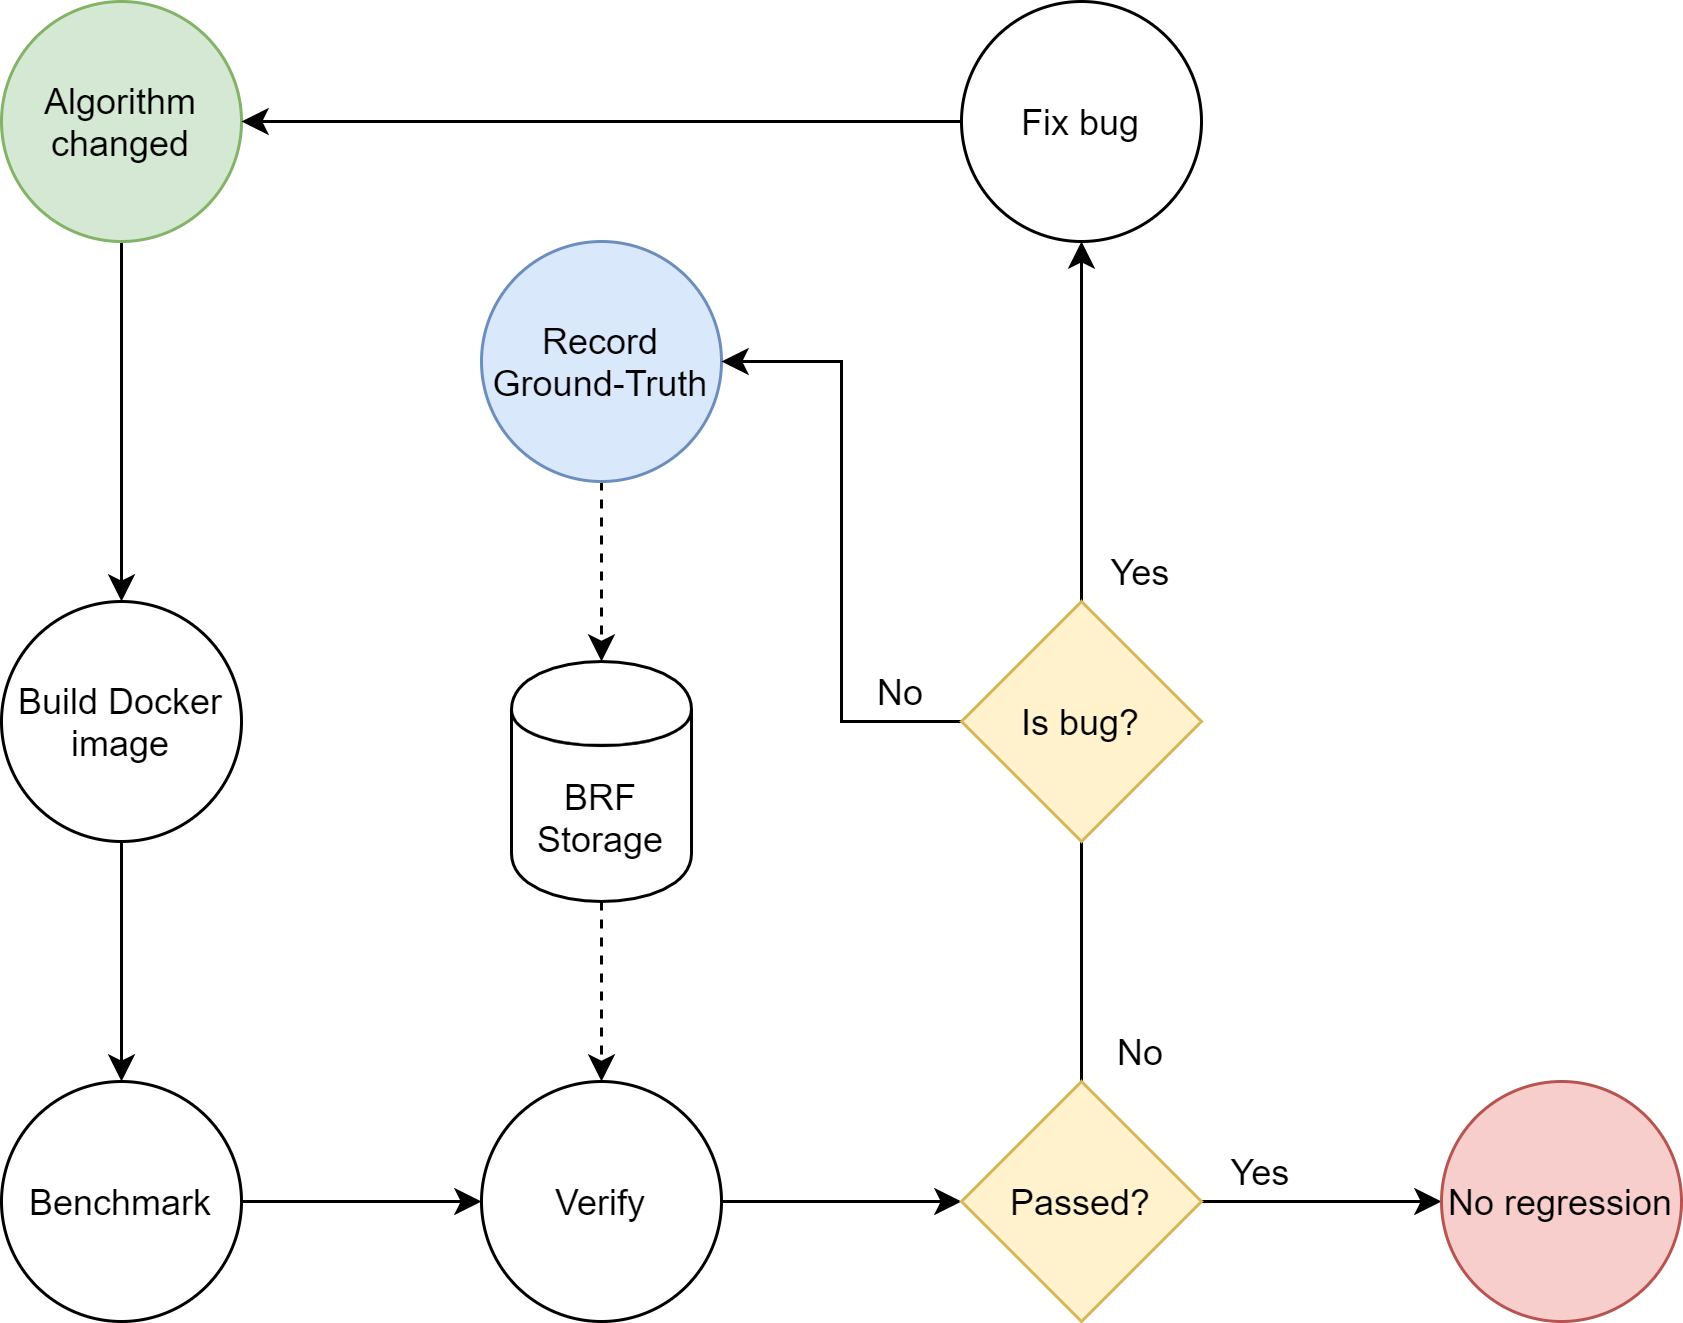
\includegraphics[width=\linewidth]{./img/crayon_for_regression_testing.png}
  \caption{Using Crayon benchmark and verify to protect against accuracy regressions. Initially a ground truth benchmark (in blue) need to be recorded. Therafter, whenever a code change occurs (in green), the algorithm is tested with Crayon through the \textit{crayon.benchmark} \& \textit{crayon.verify} functions.}
  \label{fig:crayon_as_test}
\end{figure}

\subsection{Scope and Limitations}
Since the main goal of this thesis is to perform a emprical comparison of forecasting methods, the study made in this section is deliberately small scaled. It serves as a proof of concept of how a benchmarking tool such as Crayon can be applied to other domains such as automated testing during development of time series forecasing algorithms. Furthermore, since executing all of the 400 training jobs required for a complete benchmark removes valuable time from the empirical comparison, the datasets used were the \textit{electricity} and the \textit{m4\_daily}.

\subsection{Methodology}
To evaluate Crayon for catching accuracy regressions, three Docker images of Gluon-TS is required. One image containing the code before the regression occured, the second image contains the version of Gluon-TS where the DeepAREstimator suffered an accuracy regression. The third image contains the version of Gluon-TS where the issue was fixed. These three images are hereby referred to as \textit{ground-truth image}, \textit{bugged image} and \textit{post-fix image}. Benchmarks using these three images are then performed and the generated BRFs are stored. Then each benchmark is verified against all other benchmarks with the results summarized into a table. All Docker images are then pushed to the public Dockerhub repository \textit{arangatang/masterthesis} \cite{dockerhub_arangatang}.


\subsection{Result}
In Table \ref{tab:crayon_for_accuracy_regressions} the results from the study are presented. The results show that the accuracy regression is successfully detected by the KS test for each metric since the verification passes 0 out of 3 times when comparing the \textit{pre-bug} image with the \textit{bugged} image across all metrics. Figure \ref{fig:crayon_as_test_deepar_all_rmse_solar} shows violin plots of the RMSE distributions for the three images on the \textit{Solar Energy} dataset. This plot shows that the change in distribution for the RMSE distribution between the bugged and the other images is substantial. Thus it makes sense that the KS test detected this, however, in this scenario a simpler test such as the naive approach investigated in Section \ref{sec:compairing_hypothesis_tests} should suffice.


\begin{table}[htb]
  \centering
  \begin{tabular}{cccc}
    DeepAR version & \rothalf{Pre-Bug}     & \rothalf{Bugged}     & \rothalf{Post-Fix}   \\ [0.5ex]
    \hline
    \multicolumn{4}{c}{\cellcolor{gray!25}MAPE}                                          \\
    \hline
    Pre-Bug        & \cellcolor{green}3/3  & -                    & -                    \\
    Bugged         & \cellcolor{green}0/3  & \cellcolor{green}3/3 & -                    \\
    Post-Fix       & \cellcolor{green}3/3  & \cellcolor{green}0/3 & \cellcolor{green}3/3 \\
    \multicolumn{4}{c}{\cellcolor{gray!25}MASE}                                          \\
    \hline
    Pre-Bug        & \cellcolor{green}3/3  & -                    & -                    \\
    Bugged         & \cellcolor{green}0/3  & \cellcolor{green}3/3 & -                    \\
    Post-Fix       & \cellcolor{orange}1/3 & \cellcolor{green}0/3 & \cellcolor{green}3/3 \\
    \multicolumn{4}{c}{\cellcolor{gray!25}Absolute Error}                                \\
    \hline
    Pre-Bug        & \cellcolor{green}3/3  & -                    & -                    \\
    Bugged         & \cellcolor{green}0/3  & \cellcolor{green}3/3 & -                    \\
    Post-Fix       & \cellcolor{green}3/3  & \cellcolor{green}0/3 & \cellcolor{green}3/3 \\
    \multicolumn{4}{c}{\cellcolor{gray!25}RMSE}                                          \\
    \hline
    Pre-Bug        & \cellcolor{green}3/3  & -                    & -                    \\
    Bugged         & \cellcolor{green}0/3  & \cellcolor{green}3/3 & -                    \\
    Post-Fix       & \cellcolor{orange}1/3 & \cellcolor{green}0/3 & \cellcolor{green}3/3 \\
    \multicolumn{4}{c}{\cellcolor{gray!25}MSIS}                                          \\
    \hline
    Pre-Bug        & \cellcolor{green}3/3  & -                    & -                    \\
    Bugged         & \cellcolor{green}0/3  & \cellcolor{green}3/3 & -                    \\
    Post-Fix       & \cellcolor{orange}1/3 & \cellcolor{green}0/3 & \cellcolor{green}3/3 \\
    \hline
  \end{tabular}
  \caption{Number of successfull benchmark verifications for three versions of DeepAR, two without bugs, one with. The benchmarks ran on the \textit{Electricity}, \textit{Solar Energy} and \textit{M4 Daily} datasets and error metric distributions were collected for five different error metrics on each. Optimal results marked in Green, partially optimal results are shown in Orange.}
  \label{tab:crayon_for_accuracy_regressions}
\end{table}

\begin{figure}[h]
  \centering
  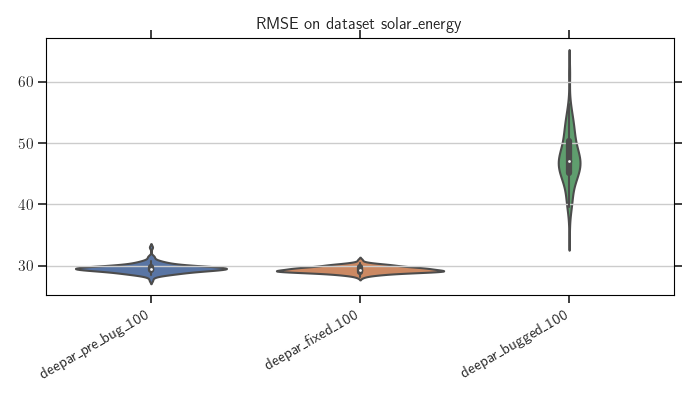
\includegraphics[width=\linewidth]{./img/crayon_study/RMSE_all_solar.png}
  \caption{Violin plots of the RMSE error distributions for the three versions of DeepAR on the solar dataset.}
  \label{fig:crayon_as_test_deepar_all_rmse_solar}
\end{figure}

The data in Table \ref{tab:crayon_for_accuracy_regressions} also shows that the \textit{bugged} image fails verification with the \textit{post-fix} image which is expected as the bug should be resolved. However, comparing the \textit{post-fix} image with the \textit{pre-bug} image fails on the \textit{M4 Daily} and the \textit{Solar Energy} datasets. This means that either the performance of DeepAR changed over the course of the 2 months between the patch or that the samples used were too few so that the KS test was unstable.

To investigate this, violin plots of the \textit{pre-bug} and the \textit{post-fix} error distributions were generated. In Figure \ref{fig:crayon_as_test_deepar_prepost_solar} two of these are presented, one for the MSIS error metric and one for the RMSE error metrics. From these, it seems that the MSIS distribution changed during the two months that the bug was present. Furthermore, it makes sense that the KS metric classified the \textit{pre-bug} metric and the \textit{post-fix} distributions as being sampled from different populations since the mean and variance of the samples differ substantially. However for the RMSE violin plots the difference is not as clear cut.

In total there were 43 commits added to Gluon-TS in the two months when the accuracy regression happened \cite{gluonts-github}. Three of them are possible causes of the detected change in accuracy between the \textit{pre-bug} and \textit{post-fix} versions. The first of these enabled multiprocessing for backtesting, as discussed in Section \ref{subsec:sources_randomness} multiprocessing can introduce additional data shuffling which can affect performance. The second change was to how the Negative Binomial was calculated and the third was a change to how MSIS error metrics was calculated. All three of these changes has immediate effect on the error distributions being tested, thus, this indicates that a second accuracy change occurred and that the KS test did not become unstable. Further investigation is needed to verify this further, however due to the time consuming process of benchmarking deepar multiple times more, this is left for future work.

To summarize, the results show that the KS test successfully identified the accuracy regression introduced on the 7th of May. Furthermore, it may have identified a second accuracy change introduced during the time the investigated bug was unnoticed. This result indicates that the benchmark and verification systems in Crayon are suitable for detecting accuracy regressions during development of time series forecasting models in time series forecasting frameworks such as Gluon-TS.

% \begin{figure}[h]
%   \centering
%   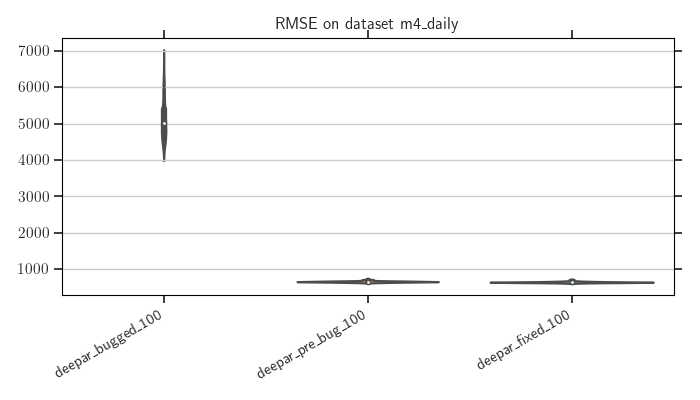
\includegraphics[width=\linewidth]{./img/crayon_study/RMSE_all_m4.png}
%   \caption{Violin plots of the RMSE error distributions for the three versions of DeepAR on the M4 dataset.}
%   \label{fig:crayon_as_test_deepar_rmse_all_m4}
% \end{figure}



% \begin{figure}[h]
% \centering
%   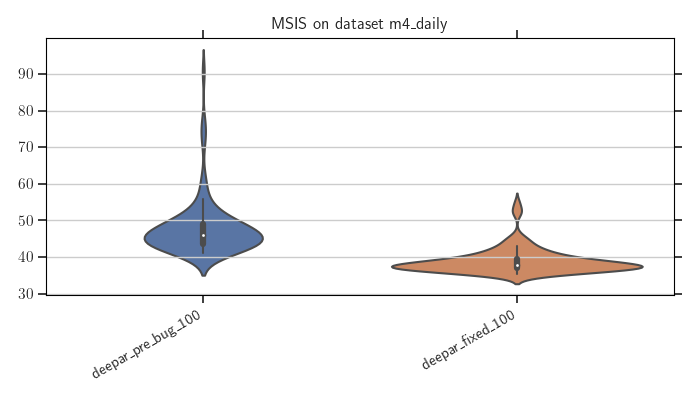
\includegraphics[width=\linewidth]{./img/crayon_study/MSIS_pre_and_fixed_m4.png}
%   \caption{Violin plots of the RMSE error distributions for the three versions of DeepAR on the solar dataset.}
%   \label{fig:crayon_as_test_deepar_prepost_msis_m4}
% \end{figure}


% \begin{figure}[h]
%   \centering
%   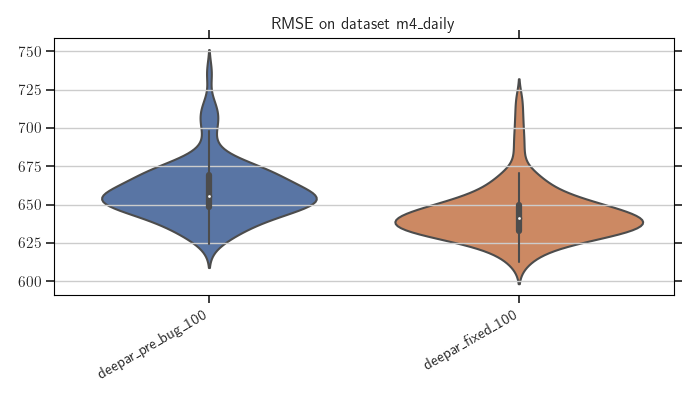
\includegraphics[width=\linewidth]{./img/crayon_study/RMSE_pre_and_fix_m4.png}
%   \caption{Violin plots of the RMSE error distributions for the three versions of DeepAR on the solar dataset.}
%   \label{fig:crayon_as_test_deepar_prepost_rmse_m4}
% \end{figure}
\begin{figure}[ht]
  \centering
  \begin{minipage}[b]{0.95\linewidth}
    \centering
    \includegraphics[width=\linewidth]{./img/crayon_study/RMSE_pre_and_fixed_solar.png}
    % \vspace{4ex}
  \end{minipage}%% 

  \begin{minipage}[b]{0.95\linewidth}
    \centering
    \includegraphics[width=\linewidth]{./img/crayon_study/MSIS_pre_and_fixed_solar.png}
    % \vspace{4ex}
  \end{minipage}
  \caption{Violin plots of the RMSE and MSIS error distributions on the solar dataset for the \textit{fixed} and \textit{pre-bug} versions of DeepAR.}
  \label{fig:crayon_as_test_deepar_prepost_solar}
\end{figure}
% \begin{figure}[h]
%   \centering
%   \includegraphics[width=\linewidth]{./img/crayon_study/MSIS_pre_and_fixed_solar.png}
%   \caption{Violin plots of the RMSE error distributions for the three versions of DeepAR on the solar dataset.}
%   \label{fig:crayon_as_test_deepar_prepost_msis_solar}
% \end{figure}

% \begin{figure}[h]
%   \centering
%   \includegraphics[width=\linewidth]{./img/crayon_study/RMSE_pre_and_fixed_solar.png}
%   \caption{Violin plots of the RMSE error distributions for the three versions of DeepAR on the solar dataset.}
%   \label{fig:crayon_as_test_deepar_prepost_rmse_solar}
% \end{figure}

\chapter{Empirical Comparison\label{cha:chapter6}}

This chapter makes use of the tools and concepts investigated in Chapters \ref{cha:approach}, \ref{cha:designing}, \ref{cha:crayon} to perform an empirical comparison of forecasting methods. Specifically, the tuning and benchmarking capabilities of Crayon are used to enable fair, accurate and reproducible comparisons. The forecasting models compared in this Section are those available in GluonTS as of March 18th 2021.


\section{Methodology}
In order to benchmark the forecasting models in GluonTS, Docker images containing GluonTS have to be built. For this the official dockerfiles available in GluonTS are used.  After the images are built, methods of speeding up backtesting are investigated. This is done since several thousands of training jobs are required to run, thus, minimizing the time to backtest saves days of training time. Three different methods of speedup are investigated; GPU acceleration, multiprocessing on CPU and using ultraJSON (ujson) package for serializing and deserializing JSON data. The ujson package is used by GluonTS if installed but is not required as the JSON package from the Python standard library is used by default \cite{gluonts-github}.

After identifying a fast performing configuration the algorithms to benchmark are identified. Due to the size of the comparison, and since the time required to tune and benchmark models differ, a priority list is followed. As the focus of the comparison is on DL based forecasting, those methods utilizing DNNs, CNNs or RNNs have the highest priority. Second highest priority are for recent forecasting models not based on DL. Thereafter, naive methods are chosen as these are quick to evaluate and serve as a good baseline to compare to. After the naive models, classical models such as arima are chosen since these only serve as a source of comparison but are not the focal point of this thesis.

When the models to benchmark are identified, these are tuned to the four datasets chosen in Chapter \ref{cha:designing} using the grid-search functionality in Crayon. The hyperparameter search space is limited for this comparison as several models are to be tuned within a few months on a single machine. Thus in order to ensure that the algorithms are optimally tuned, no limit will be put on the amount of time taken for tuning the algorithms. However, the maximum number of configurations in the grid is set to 300 and the maximum number of different values tested for a single hyperparameter was set to maximum 3. These two limits are imposed as they introduce limits for both models with few hyperparameters and models with multiple hyperparameters as discussed in Section \cite{dockerhub_arangatang}. Furthermore, hyperparameters used for all forecasting models in GluonTS share were tuned in the same way for all models for consistency.

Certain information such as the cardinality of a dataset, the prediction length and the frequency of the data are provided as metadata by the datasets in GluonTS. These values are used when performing the tuning and benchmarking for this comparison.

When using the Grid Search functionality in Crayon, runtool configurations for each tuning job is stored. When the grid-search has finished the configs of the best hyperparameter configurations are then combined into a single Runtool config file. This file is then passed to the Crayon benchmarking system so that the algorithms can be benchmarked using the optimal hyperparameters for each dataset. The BRF generated by the benchmarks are then uploaded to the public GitHub repository of the masterthesis \cite{}.

The specification of the computer used to backtest the different models and relevant software used is presented in Table \ref{tab:sys_spec}.

\begin{table}[htb]
    \centering
    \begin{tabular}{cc}
        \hline
        Component Name     & Component Used                           \\[0.5ex]
        \hline
        CPU                & I7-9700K up to 4.9 GHz                   \\
        GPU                & Nvidia Titan RTX                         \\
        CUDA Version       & 11.2                                     \\
        GPU Driver Version & 460.73.01                                \\
        RAM                & 32 GB DDR4, 3600 MHz                     \\
        Operating System   & Ubuntu 20.04.2                           \\
        Docker Version     & 20.10.6                                  \\
        GluonTS commit     & 4d1a9a09048b1e0db93de885e9636e4add8f91c6 \\
    \end{tabular}
    \caption{Specification of hardware and software used to perform the benchmarks.}
    \label{tab:sys_spec}
\end{table}

\section{Scope and limitations}
To limit the scope of this investigation, only algorithms available in GluonTS were used. Further, only a subset of these could be used due to the time limit of the thesis. As discussed in Section \ref{cha:approach} fair comparisons of advanced algorithms can only be done if the implementations being evaluated are well implemented. Since the algorithms implemented in GluonTS are implemented and used by experienced practitioners in the field of forecasting these algorithms are considered to fulfill this criteria. Only algorithms available in GluonTS up until commit: \textit{4d1a9a09048b1e0db93de885e9636e4add8f91c6} are used for the comparison, any algorithms added at a later time are not considered \cite{gluonts-github}.

Due to the limited time of the thesis in comparison to the number of algorithms which should be compared, not all algorithms in GluonTS can be tuned and benchmarked in time. Further, multivariate algorithms are not compared since GluonTS does not offer any multivariate datasets. Further only three multivariate models are available in GluonTS, GPVar, GPVar and LSTNet. Any comparisons made with these when executed on the datasets identified in \ref{sec:dataset_analysis} would be unfair since only univariate data would be used to train them.

\section{Result}
The initial task of optimizing the Docker images such that they perform well took considerably longer than anticipated. Particularly the use of GPU acceleration was problematic since certain forecasting models such as the \textit{MQCNNEstimator} failed to converge when training. Advice posted on the GluonTS Github page suggested that this issue could be resolved by lowering the learning rate, despite this the issue remained \cite{gluonts-github}. Due to the increased instability, GPU acceleration was deemed unsuitable for the comparison.

The use of the Python package \textit{ujson} showed significant speedup and no negative effects were noticed. Thus, \textit{ujson} is added to the Docker images used for benchmarking and tuning.

Initially, the multiprocessing support when using GluonTS within a Docker image was limited. This caused backtesting to fail sporadically. The underlying cause for this was investigated and a pull request solving this was opened \cite{fix_dockerfile_pr}. While this made multiprocessing stable, the number of threads used could only be controlled up to 4, if more threads vere requested than four it had no effect as the CPU utilization remained the same. However, executing the models on four cores instead of one did improve throughput significantly and was thus utilized for the benchmarks.

Most of the algorithms in GluonTS can be executed through the same Docker image. However, the naive forecasting algorithms, the Prophet forecaster, and the classical models had additional dependencies. Thus in total four Docker images were built. These images are available on the \textit{arangatang/masterthesis} repository on Dockerhub \cite{dockerhub_arangatang}.

Of the 20 algorithms presented in Section \ref{algorithms} four does not require tuning; Prophet, Naive Seasonal, Naive 2 and the Theta from the RForecastPredictor. Since multivariate algorithms are excluded from the study, the GPVAREstimator, DeepVAREstimator and the LSTNET estimators are not tuned. In order to tune the remaining 13 models, 920+ configurations were executed on 4 datasets with 3 repetitions per hyperparameter configuration. Thus, more than 11000 training jobs were executed over the course of four months. An overview of the results from the tuning is presented in Table \ref{tab:tuning_results}.

\begin{table}[htb]
    \centering
    \begin{tabular}{cccccc}
        Algorithm         & \rothalf{Electricity} & \rothalf{Solar Energy} & \rothalf{M4 Daily}   & \rothalf{M5}         & \rothalf{Electricity (GPU)} \\
        \hline
        DeepAR            & \cellcolor{green}X    & \cellcolor{green}X     & \cellcolor{green}X   & \cellcolor{green}X   & \cellcolor{green}X          \\
        DeepFactor        & \cellcolor{green}X    & \cellcolor{green}X     & \cellcolor{green}X   & \cellcolor{green}X   & \cellcolor{green}X          \\
        CanonicalRNN      & \cellcolor{green}X    & \cellcolor{green}X     & \cellcolor{green}X   & \cellcolor{green}X   & \cellcolor{green}X          \\
        SimpleFeedForward & \cellcolor{green}X    & \cellcolor{green}X     & \cellcolor{green}X   & \cellcolor{green}X   & \cellcolor{green}X          \\
        NBEATS Ensamble   & \cellcolor{green}X    & \cellcolor{green}X     & \cellcolor{green}X   & \cellcolor{green}X   & \cellcolor{green}X          \\
        Gaussian Process  & \cellcolor{green}X    & \cellcolor{green}X     & \cellcolor{green}X   & \cellcolor{red} F    & \cellcolor{green}X          \\
        MQCNN             & \cellcolor{green}X    & \cellcolor{green}X     & \cellcolor{green}X   & \cellcolor{green}X   & \cellcolor{red} F           \\
        MQRNN             & \cellcolor{green}X    & \cellcolor{green}X     & \cellcolor{green}X   & \cellcolor{green}X   & \cellcolor{green}X          \\
        Transformer       & \cellcolor{green}X    & \cellcolor{green}X     & \cellcolor{green}X   & \cellcolor{green}X   & \cellcolor{green}X          \\
        DeepState         & \cellcolor{orange}M   & -                      & -                    & -                    & \cellcolor{orange}M         \\
        WaveNet           & \cellcolor{red}F      & -                      & -                    & -                    & \cellcolor{red}F            \\
        NPTS              & \cellcolor{red}F      & -                      & -                    & -                    & \cellcolor{red}F            \\
        Seq2Seq           & -                     & -                      & -                    & \cellcolor{red}F     & -                           \\
        Prophet           & \cellcolor{blue!25}U  & \cellcolor{blue!25}U   & \cellcolor{blue!25}U & \cellcolor{blue!25}U & \cellcolor{blue!25}U        \\
        Naive Seasonal    & \cellcolor{blue!25}U  & \cellcolor{blue!25}U   & \cellcolor{blue!25}U & \cellcolor{blue!25}U & \cellcolor{blue!25}U        \\
        Naive2            & \cellcolor{blue!25}U  & \cellcolor{blue!25}U   & \cellcolor{blue!25}U & \cellcolor{blue!25}U & \cellcolor{blue!25}U        \\
        Theta             & \cellcolor{blue!25}U  & \cellcolor{blue!25}U   & \cellcolor{blue!25}U & \cellcolor{blue!25}U & \cellcolor{blue!25}U        \\
        \hline
    \end{tabular}
    \caption{Tuning results of 16 forecasting algorithms in GluonTS. Legend: X (green) finished successfully, M (orange) memory leak, F (red) failed, U (blue) tuning not required.}
    \label{tab:tuning_results}
\end{table}

Of the 13 models which required tuning, 7 were tuned without major issues, however for five of the algorithms; Gaussian Process (GP), DeepState, WaveNet, NPTS and Seq2Seq harder issues arose when executing on CPU. The issue with the GP Estimator stemmed from how the \textit{cardinality} hyperparameter was passed. For all other algorithms in GluonTS the cardinality is passed as a list of integers but the GP Estimator requires a single integer to be passed. This is easily fixed for three out of the four datasets as the cardinality stored in the datasets metadata only contained one value. However, the metadata of the M5 dataset contained multiple values in the cardinality. Thus, the GP estimator failed to execute for the M5 dataset. WaveNet failed due to multiprocessing issues, since considerable time had been spent in fixing the multiprocessing system, debugging the WaveNet algorithm and tuning it was considered to take too much time, investigating it further was thus put on hold. The NPTS algorithm failed due to compatibility issues with the GluonTS shell, fixing this was considered outside the scope of the thesis. The Seq2Seq estimator was one of the last estimators to be tuned, when it failed not much time was left to tune the models thus, the Seq2Seq estimator was excluded from the comparison. The tuning of DeepState was cancelled when all of the available 32 GB of RAM and 32 GB of swap had been utilized. This happened before the first training epoch was finished. Thus it is unclear whether the DeepState estimator suffered a memory leak or if it had unusually high memory requirements compared to the other algorithms in GluonTS. An overview of the tuning results is presented in Table \ref{tab:tuning_results}.

After the tuning of the algorithms finished,  the 13 remaining algorithms were benchmarked through crayon. This resulted in 5600 training jobs being executed over the course of two months. Tables; \ref{tab:benchmark_results_MASE_MAPE}, \ref{tab:benchmark_results_abs_rmse} and \ref{tab:benchmark_results_msis} present the results of these for the MASE, MAPE, RMSE, MSIS and Absolute error metrics. These error metrics are aggregated using the RMSE4D methods as described in Section \ref{sec:ranking_distributions}. In Table \ref{tab:mean_ranks} the average rank of each benchmark is presented to summarize Tables \ref{tab:benchmark_results_MASE_MAPE}, \ref{tab:benchmark_results_abs_rmse} and \ref{tab:benchmark_results_msis}.

\begin{table}[h]
    \centering
    \pgfplotstabletypeset[
        color cells={min=0,max=11.05},
        col sep=comma,
        columns/Algorithm/.style={reset styles,string type},
        columns/Mean Rank/.style={reset styles,string type},
        /pgfplots/colormap={whiteblue}{rgb255(0cm)=(255,255,255); rgb255(1cm)=(0,128,255)},
        /pgf/number format/.cd,
        fixed,
        fixed zerofill,
        precision=2,
    ]{
        Algorithm, MASE, MAPE, RMSE, Absolute Error, MSIS, Mean Rank
        DeepAR, 3.25, 6.75, 3.00, 4.00, 2.25, 3.80
        NBEATS, 2.50, 5.50, 3.75, 2.25, 6.00, 3.90
        Transformer, 3.50, 6.75, 4.25, 4.50, 2.75, 4.25
        SimpleFF, 4.75, 5.75, 4.50, 5.50, 2.25, 4.45
        MQCNN, 6.00, 5.50, 4.50, 4.75, 11.00, 6.15
        C-RNN, 6.75, 8.00, 6.50, 6.50, 4.25, 6.30
        S-Naive, 6.75, 4.75, 7.75, 6.25, 7.75, 6.30
        Thetaf, 6.50, 2.75, 5.75, 6.50, 7.50, 6.90
        Naive2, 8.50, 6.50, 10.25, 8.50, 8.50, 8.10
        DeepFactor, 10.00, 8.75, 9.75, 10.00, 7.00, 8.60
        MQRNN, 9.25, 8.00, 9.25, 9.00, 11.00, 8.95
        GP, 10.75, 8.75, 10.25, 10.75, 9.00, 9.55
        Prophet, 12.00, 12.00, 11.00, 12.00, 8.25, 11.05
    }
    \caption{Mean ranks of the benchmarks for the MASE, MAPE, RMSE, Absolute Error and MSIS error metrics.}
    \label{tab:mean_ranks}
\end{table}

As presented in Table \ref{tab:mean_ranks} DeepAR is the algorithm with the best average ranking across all datasets and error metrics. Since DeepAR automatically applies categorical features to the dataset it may have gained an upper hand in this comparison since this data is not part of the datasets used. The source paper of DeepAR evaluates DeepAR on the Electricity dataset, however, the metric used is a modified version of RMSE known as nRMSE which makes it impossible to compare the results as the metrics have different scales. However in the M5 competition, a modified version of DeepAR was the third best performing forecasting algorithm. This reinforces the findings from this research since DeepAR was the second best performer for the M5 dataset on three out of the five error metrics and the fourth best on the MSIS metric.

The NBEATS Ensemble Estimator is the second best performer with an average rank between 2 - 6 across all tested metrics. While it generally performed well, its performance on the M4 Daily dataset was average to poor (between 4-10). This implies that NBEATS may be unsuited for heavily trended data and may thus benefit from detrending the data beforehand. In the original paper of NBEATS it is evaluated on the M4 dataset, however not only on the \textit{M4 daily} data as has been done here but on the complete M4 dataset. This in combination with them utilizing a modified MAPE metric (sMAPE) for ranking their results makes comparing results hard. They do however show that NBEATS perform better than Theta on the M3 dataset. This can be seen in the results from this benchmark as well for the Electricity and Solar Energy datasets. For the M4 Daily dataset, this is however not the case as Theta performs better than NBEATS for all metrics. Not only is theta better than NBEATS on the M4 Daily, both of the Naive approaches also outperform NBEATS and all other DL models for the Absolute Error, MASE and MAPE metrics on the M4 Daily dataset.

The Transformer forecaster is the third best ranked algorithm and has the 2nd best MSIS score of all tested algorithms after DeepAR and Simple Feed Forward which is the fourth best performing algorithm. This indicates that these two algorithms sacrifice specificity of forecasts in exchange for better coverage of the probability intervals. I.e. their forecasts are less often spot on but rarely very wrong. It is surprising that SimpleFF ranked so high in this comparison as it outperformed more sophisticated DL approaches like the MQCNN, MQRNN and DeepFactor with its simple neural architecture. Furthermore, the performance of the SimpleFF also outperformed the C-RNN architecture despite C-RNN containing LSTM cells which tends to be better for temporal data such as time series. Possibly, C-RNN overfit to the datasets when tuning as the hyperparameters configuration found when tuning were larger neural nets with more cells for the smaller datasets and smaller nets for the larger datasets. For the datasets where C-RNN performed worst, \textit{M4 Daily \& Electricity} 210 cells were used compared to 100 for \textit{M5 \& Solar Energy}.

MQCCN was the fifth best performing algorithm, with a mean rank of 6.15. It should be noted that the MSIS error was not reported by GluonTS for either MQCNN or MQRNN and that their ranks suffered as a result. This is counterintuitive as both of these produce probabilistic forecasts which means calculating the MSIS should be without issues. Recalculating the mean rank for these two algorithms without MSIS would cause MQCNN to have a mean rank of 5.19 and MQRNN 8.875 instead of 8.95, thus, their overall ranks would remain the same in this comparison. One possible reason why these two models are not ranked higher in this comparison is due to the lack of exogenous data when training the model. In the original paper of these algorithms, the authors manually added calendar features such as holidays and which day of the week each datapoint in the datasets were recorded on \cite{wen_multi-horizon_2018}.

The Theta Forecaster was developed to function well for the M3 dataset, thus, it is not surprising that it performs the best of all tested models on the M4 dataset as the M4 dataset is similar in composition to the M3 dataset but larger \cite{m3_vs_M4}. The performance of Thetaf was however in the bottom 50\% for the other datasets, which indicates that while it performs well for datasets having high trend and low seasonality, such as the M4,  it does not generalize well to datasets with other characteristics. Particularly this is seen for highly seasonal datasets such as the Solar Energy dataset and the Electricity datasets where theta performs in the bottom 50\%.

\begin{figure}[htb]
    \centering
    \minipage{0.5\textwidth}
    \includegraphics[width=\linewidth]{./img/solar_energy_10min_small.png}
    \caption{Solar Energy timeseries with frequency 10 min.}
    \label{fig:solar_10_min}
    \endminipage\hfill
    \minipage{0.5\textwidth}
    \includegraphics[width=\linewidth]{./img/solar_energy_fixed_small.png}
    \caption{Solar Energy timeseries with frequency 1 hour.}
    \label{fig:solar_fixed}
    \endminipage\hfill
\end{figure}

The S-Naive forecaster performed well on the Electricity and the M4 daily dataset with average ranks of 3.4 and 3.6 respectively. However for the Solar Energy dataset the average rank across all metrics was 8.6. This does not make sense as the solar energy dataset has the highest strength of seasonality of all datasets. Thus sampling values from previous seasons as is done in the S-Naive forecaster should bring competitive performance at least on par with the performance of S-Naive on the other datasets. After investigating this further an issue with the Solar Energy dataset in GluonTS was identified. The frequency the dataset is sampled with is 10 minutes according to the metadata. However, this could be a mistake and that the data has a frequency of 1H. In Figure \ref{fig:solar_10_min} a time series from the dataset is shown plotted using a frequency of 10 minutes. If the true frequency of the data would be 10 minutes, then the power production of the solar panels spikes for two hours and then produces zero energy for two hours. Since solar panels produce power when the sun is out during the day and not when it is night, these two hours cycles would mean that the day is two hours long. By setting the frequency to \textit{1H} instead of the original \textit{10min} the timeseries is properly aligned as in Figure \ref{fig:solar_fixed}. This is a likely cause as to why the Seasonal Naive performed poorly on the Solar Energy dataset. Since the Thetaf forecaster deseasonalizes each time series when it is run, the ranking of this could have been affected as well. The faulty frequency to the Solar Energy dataset also likely caused the automatic feature engineering in DeepAR to add calendar features to the wrong parts of the data, i.e. marking datapoints sampled in April to be sampled in December.

The second naive model, Naive2, crashed on the Electricity dataset due to it utilizing multiplicative decomposition of time series which is not suitable for time series data close to 0. The API for this model in GluonTS does not support additive decomposition, thus not much could be done to fix this. The average rank of the Naive2 method was 8.10 which makes it that fourth worst performing method of the ones tested.

The low rank of DeepFactor contradicts the results from its original paper as there, DeepFactor, outperformed DeepAR on average while in Table \ref{tab:mean_ranks} DeepAR outperforms all other algorithms. This further enforces the benefit of automatically adding exogenous variables such as calendar days and holidays to the data like DeepAR does. The original paper of DeepFactor also compares it against MQRNN and Prophet, their findings do align with the results of this comparison since DeepAR has a better average rank than both. However, Prophet did not have time to finish the benchmark on the \textit{M5} and \textit{Electricity} datasets so comparing these only by looking at the mean ranks is not fair. Comparing the mean ranks of DeepFactor and Prophet across all metrics for the Solar Energy and the M4 Daily datasets tells a similar story where DeepFactor recieves an average rank of \(10+11.5+10+9.5+9=10\) and Prophet receives the mean rank \(12+12+12+10+6.5=10.5\). Thus, for this comparison, DeepFactor is only marginally better than Prophet.

The Gaussian Process (GP) forecasting method was ranked second last, with Prophet in the last place. The GP method was suboptimally tuned as the kernel used for creating the Gaussian Processes could not be specified through the GluonTS shell when tuning. This may have led to a subpar kernel being used for the benchmark.

\begin{table}[htb]
    \centering
    \begin{tabular}{ccccccc}
        Algorithm   & \rothalf{Electricity} & \rothalf{Solar Energy} & \rothalf{M4 Daily} & \rothalf{M5} & \rothalf{Mean rank} \\
        \hline
        \multicolumn{6}{c}{\cellcolor{gray!25}MSIS}                                                                            \\
        \hline
        DeepAR      & 6.44 (1)              & 8.55 (2)               & 43.13 (2)          & 32.58 (4)    & 2.25                \\\hline
        SimpleFF    & 10.64 (3)             & 14.78 (3)              & 36.33 (1)          & 26.49 (2)    & 2.25                \\\hline
        Transformer & 6.85 (2)              & 6.41 (1)               & 49.15 (3)          & 35.38 (5)    & 2.75                \\\hline
        C-RNN       & 21.96 (4)             & 46.74 (6)              & 105.21 (4)         & 31.41 (3)    & 4.25                \\\hline
        NBEATS      & 33.35 (5)             & 46.50 (5)              & 137.24 (8)         & 57.74 (6)    & 6.00                \\\hline
        DeepFactor  & 479.13 (9)            & 53.17 (7)              & 928.47 (11)        & 20.78 (1)    & 7.00                \\\hline
        Thetaf      & 47.02 (7)             & 97.08 (11)             & 130.49 (5)         & 69.13 (7)    & 7.50                \\\hline
        S-Naive     & 35.25 (6)             & 97.07 (9)              & 131.14 (7)         & 81.28 (9)    & 7.75                \\\hline
        Prophet     & nan (10)              & 20.84 (4)              & 166.84 (9)         & nan (10)     & 8.25                \\\hline
        Naive2      & nan (10)              & 97.07 (10)             & 131.14 (6)         & 81.28 (8)    & 8.50                \\\hline
        GP          & 126.45 (8)            & 84.13 (8)              & 185.82 (10)        & nan (10)     & 9.00                \\\hline
        MQRNN       & nan (10)              & nan (12)               & nan (12)           & nan (10)     & 11.00               \\\hline
        MQCNN       & nan (10)              & nan (12)               & nan (12)           & nan (10)     & 11.00               \\\hline
    \end{tabular}
    \caption{Benchmark results with respects to the MSIS error metric. Ranks within a dataset shown in parentheses.}
    \label{tab:benchmark_results_msis}
\end{table}


\begin{table}[htb]
    \centering
    \begin{tabular}{ccccccc}
        Algorithm   & \rothalf{Electricity} & \rothalf{Solar Energy} & \rothalf{M4 Daily} & \rothalf{M5} & \rothalf{Mean rank} \\
        \hline
        \multicolumn{6}{c}{\cellcolor{gray!25}MASE}                                                                            \\
        \hline
        NBEATS      & 0.83 (3)              & 1.16 (2)               & 3.43 (4)           & 1.44 (1)     & 2.50                \\\hline
        DeepAR      & 0.75 (1)              & 1.17 (3)               & 3.81 (7)           & 1.48 (2)     & 3.25                \\\hline
        Transformer & 0.82 (2)              & 1.13 (1)               & 4.26 (8)           & 1.50 (3)     & 3.50                \\\hline
        SimpleFF    & 0.92 (5)              & 1.27 (4)               & 3.48 (5)           & 1.54 (5)     & 4.75                \\\hline
        MQCNN       & 1.22 (7)              & 1.50 (5)               & 3.51 (6)           & 1.55 (6)     & 6.00                \\\hline
        Thetaf      & 1.18 (6)              & 2.43 (11)              & 3.26 (1)           & 1.73 (8)     & 6.50                \\\hline
        S-Naive     & 0.88 (4)              & 2.43 (10)              & 3.28 (2)           & 2.03 (11)    & 6.75                \\\hline
        C-RNN       & 2.24 (8)              & 1.60 (6)               & 4.31 (9)           & 1.52 (4)     & 6.75                \\\hline
        Naive2      & nan (12)              & 2.43 (9)               & 3.28 (3)           & 2.03 (10)    & 8.50                \\\hline
        MQRNN       & 11.19 (10)            & 1.71 (7)               & 57.94 (13)         & 1.58 (7)     & 9.25                \\\hline
        DeepFactor  & 12.02 (11)            & 1.84 (8)               & 23.64 (12)         & 1.85 (9)     & 10.00               \\\hline
        GP          & 3.18 (9)              & 2.45 (12)              & 4.69 (10)          & nan (12)     & 10.75               \\\hline
        Prophet     & nan (12)              & 3.26 (13)              & 11.96 (11)         & nan (12)     & 12.00               \\\hline
        \multicolumn{6}{c}{\cellcolor{gray!25}MAPE}                                                                            \\
        \hline
        Thetaf      & 0.18 (6)              & 1.00 (1)               & 0.04 (3)           & 0.65 (1)     & 2.75                \\\hline
        S-Naive     & 0.14 (4)              & 1.00 (3)               & 0.04 (1)           & 0.88 (11)    & 4.75                \\\hline
        NBEATS      & 0.13 (3)              & 2.84 (7)               & 0.05 (5)           & 0.82 (7)     & 5.50                \\\hline
        MQCNN       & 0.22 (7)              & 2.15 (6)               & 0.05 (4)           & 0.79 (5)     & 5.50                \\\hline
        SimpleFF    & 0.14 (5)              & 2.96 (8)               & 0.05 (6)           & 0.79 (4)     & 5.75                \\\hline
        Naive2      & nan (12)              & 1.00 (2)               & 0.04 (2)           & 0.88 (10)    & 6.50                \\\hline
        DeepAR      & 0.10 (1)              & 3.29 (10)              & 0.05 (7)           & 0.87 (9)     & 6.75                \\\hline
        Transformer & 0.10 (2)              & 3.27 (9)               & 0.06 (8)           & 0.86 (8)     & 6.75                \\\hline
        C-RNN       & 0.30 (8)              & 4.92 (12)              & 0.06 (9)           & 0.79 (3)     & 8.00                \\\hline
        MQRNN       & 1.01 (11)             & 1.03 (4)               & 0.42 (13)          & 0.82 (6)     & 8.50                \\\hline
        DeepFactor  & 0.99 (10)             & 4.09 (11)              & 0.20 (12)          & 0.70 (2)     & 8.75                \\\hline
        GP          & 0.34 (9)              & 1.09 (5)               & 0.06 (10)          & nan (12)     & 9.00                \\\hline
        Prophet     & nan (12)              & 8.22 (13)              & 0.15 (11)          & nan (12)     & 12.00               \\\hline
    \end{tabular}
    \caption{Benchmark results with respect to the MASE and MAPE metrics. Ranks within a dataset shown in parentheses.}
    \label{tab:benchmark_results_MASE_MAPE}
\end{table}

% \begin{adjustbox}{center}
% <your table (i.e. the tabular or similar environment)>
% \end{adjustbox}

\begin{table}[htb]
    \centering
    \begin{tabular}{ccccccc}
        Algorithm   & \rothalf{Electricity} & \rothalf{Solar Energy} & \rothalf{M4 Daily} & \rothalf{M5} & \rothalf{Mean rank} \\
        \hline
        \multicolumn{6}{c}{\cellcolor{gray!25}Absolute Error}                                                                  \\
        \hline
        NBEATS      & 8869733 (1)           & 336976 (2)             & 11201583 (5)       & 811248 (1)   & 2.25                \\\hline
        DeepAR      & 9327671 (4)           & 339306 (3)             & 12135357 (7)       & 844784 (2)   & 4.00                \\\hline
        Transformer & 9263741 (3)           & 328560 (1)             & 13681491 (9)       & 869196 (5)   & 4.50                \\\hline
        MQCNN       & 13805770 (7)          & 432799 (5)             & 11070810 (4)       & 856588 (3)   & 4.75                \\\hline
        SimpleFF    & 9531230 (5)           & 369138 (4)             & 11234445 (6)       & 904818 (7)   & 5.50                \\\hline
        S-Naive     & 8962995 (2)           & 708874 (10)            & 10701169 (2)       & 1152816 (11) & 6.25                \\\hline
        Thetaf      & 13089580 (6)          & 708907 (11)            & 10512352 (1)       & 912691 (8)   & 6.50                \\\hline
        C-RNN       & 29287248 (8)          & 465076 (6)             & 13542748 (8)       & 861390 (4)   & 6.50                \\\hline
        Naive2      & nan (12)              & 708874 (9)             & 10701169 (3)       & 1152816 (10) & 8.50                \\\hline
        MQRNN       & 121965994 (10)        & 499512 (7)             & 205836216 (13)     & 880390 (6)   & 9.00                \\\hline
        DeepFactor  & 128561908 (11)        & 531101 (8)             & 72334786 (12)      & 1025815 (9)  & 10.00               \\\hline
        GP          & 38069033 (9)          & 715938 (12)            & 15070775 (10)      & nan (12)     & 10.75               \\\hline
        Prophet     & nan (12)              & 950621 (13)            & 40508217 (11)      & nan (12)     & 12.00               \\\hline
        \multicolumn{6}{c}{\cellcolor{gray!25}RMSE}                                                                            \\
        \hline
        DeepAR      & 1752.89 (5)           & 30.81 (3)              & 637.84 (2)         & 2.28 (2)     & 3.00                \\\hline
        NBEATS      & 1177.71 (2)           & 30.53 (2)              & 748.49 (10)        & 2.21 (1)     & 3.75                \\\hline
        Transformer & 1399.50 (4)           & 29.55 (1)              & 677.32 (5)         & 2.53 (7)     & 4.25                \\\hline
        SimpleFF    & 1229.84 (3)           & 35.58 (4)              & 672.66 (3)         & 2.79 (8)     & 4.50                \\\hline
        MQCNN       & 1850.22 (6)           & 39.29 (5)              & 672.82 (4)         & 2.31 (3)     & 4.50                \\\hline
        Thetaf      & 1936.66 (7)           & 62.51 (10)             & 630.09 (1)         & 2.43 (5)     & 5.75                \\\hline
        C-RNN       & 4629.80 (8)           & 41.28 (6)              & 745.09 (8)         & 2.39 (4)     & 6.50                \\\hline
        S-Naive     & 1139.93 (1)           & 62.52 (13)             & 705.42 (6)         & 3.30 (11)    & 7.75                \\\hline
        MQRNN       & 13405.46 (10)         & 45.92 (8)              & 5443.89 (13)       & 2.53 (6)     & 9.25                \\\hline
        DeepFactor  & 13505.91 (11)         & 42.26 (7)              & 2192.18 (12)       & 2.97 (9)     & 9.75                \\\hline
        GP          & 6113.39 (9)           & 62.52 (11)             & 747.68 (9)         & nan (12)     & 10.25               \\\hline
        Naive2      & nan (12)              & 62.52 (12)             & 705.42 (7)         & 3.30 (10)    & 10.25               \\\hline
        Prophet     & nan (12)              & 53.51 (9)              & 1464.99 (11)       & nan (12)     & 11.00               \\\hline
    \end{tabular}
    \caption{Benchmark results with respect to the Absolute Error and RMSE metrics. Ranks within a dataset shown in parentheses.}
    \label{tab:benchmark_results_abs_rmse}
\end{table}

The overall result of this empirical comparison of forecasting methods showed that DeepAR, NBEATS and the Transformer forecasting methods are the  best performing forecasting methods out of the 13 investigated. Each of these 13 models were evaluated on four complimentary datasets with diverse characteristics in terms of trend and strength and on five different metrics. Furthermore, statistical and naive models were the strongest performer for the \textit{M4 Daily} dataset but underperformed compared to DL based forecasting methods on the \textit{Solar Energy, M5} and \textit{Electricity} datasets.
\chapter{Conclusion\label{cha:chapter6}}
... should include the following:
\begin{itemize}

\item problem restated and a brief summary of the methodology,
\item student contributions (e.g., survey, open-source software, journal publication),
\item a brief summary of the findings and results,
\item limitations and generalizability of the findings and results.
\item lessons learned,
\item recommendations for future research.

\end{itemize}


\chapter{Conclusion\label{cha:chapter6}}
... should include the following:
\begin{itemize}

\item problem restated and a brief summary of the methodology,
\item student contributions (e.g., survey, open-source software, journal publication),
\item a brief summary of the findings and results,
\item limitations and generalizability of the findings and results.
\item lessons learned,
\item recommendations for future research.

\end{itemize}


\chapter{Conclusion\label{cha:chapter6}}
... should include the following:
\begin{itemize}

\item problem restated and a brief summary of the methodology,
\item student contributions (e.g., survey, open-source software, journal publication),
\item a brief summary of the findings and results,
\item limitations and generalizability of the findings and results.
\item lessons learned,
\item recommendations for future research.

\end{itemize}



% ---------------------------------------------------------------

%Bibliography 
\begingroup
\raggedright
\bibliographystyle{splncs03}
%\bibliographystyle{acm}
\bibliography{bibliography}
\endgroup

%appendix
\chapter{Appendix}
\section{Example code}

\section{Heatmaps of hypothesis tests}
\label{app:heatmaps}

This section contains heatmaps generated by applying hypthesis tests to samples of varying size sampled from a distribution of error metrics generated by the DeepAREstimator on the Electricity dataset. DeepAR was executed with three different values of the \textit{distr\_output} hyperparameter; NegativeBinomialOutput, StudentTOutput and PoissonOutput. The distributions generated by the different hyperparameter configurations are refered to as Negative Binomial, Student T and Poisson. See Section \ref{hypothesis_test_methodology} for more information about how the distributions were generated.

In the heatmaps, green means the test approves the samples being from the same distribution otherwise it is red.


\subsection{Kolmogorov Smirnov heatmaps of samples from a single distribution}

\begin{figure}[htb]
  \centering
  \includegraphics[width=\linewidth]{./img/hypothesis_test/appendix/ks_neg_bin.png}
  \caption{Negative Binomial}
\end{figure}
\clearpage
\begin{figure}[htb]
  \centering
  \includegraphics[width=\linewidth]{./img/hypothesis_test/appendix/ks_poisson.png}
  \caption{Poisson}
\end{figure}
\clearpage
\begin{figure}[htb]
  \centering
  \includegraphics[width=\linewidth]{./img/hypothesis_test/appendix/ks_student_t.png}
  \caption{Student T}
\end{figure}
\clearpage

\subsection{Kolmogorov Smirnov heatmaps of samples from two independent and shuffled distributions}

\begin{figure}[htb]
  \centering
  \includegraphics[width=\linewidth]{./img/hypothesis_test/appendix/ks_X_neg_bin_Y_student_t_shuffled.png}
  \caption{Negative Binomial on X axis and Student T on Y axis}
\end{figure}
\clearpage
\begin{figure}[htb]
  \centering
  \includegraphics[width=\linewidth]{./img/hypothesis_test/appendix/ks_X_poisson_Y_neg_bin_shuffled.png}
  \caption{Poisson on X axis and Negative Binomial on Y axis}
\end{figure}
\clearpage
\begin{figure}[htb]
  \centering
  \includegraphics[width=\linewidth]{./img/hypothesis_test/appendix/ks_X_poisson_Y_student_t_shuffled.png}
  \caption{Poisson on X and Student T on Y axis}
\end{figure}
\clearpage
\subsection{Heatmaps of the naive method applied to samples of varying length from a single distribution}

\begin{figure}[htb]
  \centering
  \includegraphics[width=\linewidth]{./img/hypothesis_test/appendix/naive_neg_bin.png}
  \caption{Negative Binomial}
\end{figure}
\clearpage
\begin{figure}[htb]
  \centering
  \includegraphics[width=\linewidth]{./img/hypothesis_test/appendix/naive_poisson.png}
  \caption{Poisson}
\end{figure}
\clearpage
\begin{figure}[htb]
  \centering
  \includegraphics[width=\linewidth]{./img/hypothesis_test/appendix/naive_student_t.png}
  \caption{Student T}
\end{figure}
\clearpage
\subsection{Heatmaps of the naive method applied to samples of varying length from two independent distributions}

\begin{figure}[htb]
  \centering
  \includegraphics[width=\linewidth]{./img/hypothesis_test/appendix/naive_X_neg_bin_Y_student_t.png}
  \caption{Negative Binomial on X axis and Student T on Y axis}
\end{figure}
\clearpage
\begin{figure}[htb]
  \centering
  \includegraphics[width=\linewidth]{./img/hypothesis_test/appendix/naive_X_poisson_Y_neg_bin.png}
  \caption{Poisson on X axis and Negative Binomial on Y axis}
\end{figure}
\clearpage
\begin{figure}[htb]
  \centering
  \includegraphics[width=\linewidth]{./img/hypothesis_test/appendix/naive_X_poisson_Y_student_t.png}
  \caption{Poisson on X and Student T on Y axis}
\end{figure}
\clearpage
\subsection{Heatmaps of the T-test applied to samples of varying length from a single distribution}

\begin{figure}[htb]
  \centering
  \includegraphics[width=\linewidth]{./img/hypothesis_test/appendix/ttest_neg_bin.png}
  \caption{Negative Binomial}
\end{figure}
\clearpage
\begin{figure}[htb]
  \centering
  \includegraphics[width=\linewidth]{./img/hypothesis_test/appendix/ttest_poisson.png}
  \caption{Poisson}
\end{figure}
\clearpage
\begin{figure}[htb]
  \centering
  \includegraphics[width=\linewidth]{./img/hypothesis_test/appendix/ttest_student_t.png}
  \caption{Student T}
\end{figure}
\clearpage
\section{Dataset Plots and statistics}
\label{app:dataset_analysis}
\clearpage
\subsection{Electricity}
\begin{table}[htb]
  \begin{tabular}{||c | c c c c c c c c ||}
    \hline
    Dataset & Mean    & Series & Items    & Shortest & Longest & Min & Max      & Frequency \\ [0.5ex]
    \hline\hline
    train   & 2510.68 & 321    & 6755124  & 21044    & 21044   & 0.0 & 764000.0 & 1H        \\
    \hline
    test    & 2509.92 & 2247   & 47501580 & 21068    & 21212   & 0.0 & 764000.0 & 1H        \\
    \hline
  \end{tabular}
  \caption{Statistics of the Electricity dataset.}
\end{table}

\begin{figure}[htb]
  \centering
  \minipage{1.0\textwidth}
  \includegraphics[width=\linewidth]{./img/electricity_plot.png}
  \caption{Plot over the average timeseries in the electricity dataset with one standard deviation shown in green. Only positive values are shown as the dataset is non-negative.}
  \label{fig:electricity_plot}
  \endminipage\hfill
\end{figure}

\begin{figure}[htb]
  \centering
  \minipage{1.0\textwidth}
  \includegraphics[width=\linewidth]{./img/electricity_no_negative.png}
  \caption{Zoomed version of \ref{fig:electricity_plot}}
  \label{fig:electricity_plot_zooomed}
  \endminipage\hfill
\end{figure}

\begin{figure}[htb]
  \centering
  \minipage{0.4\textwidth}
  \begin{center}
    \begin{tabular}{||c | c | c | c | c |}
      \hline
      statistic   & mean & deviation & max & min  \\
      \hline
      trend       & 0.65 & 0.17      & 1.0 & 0.09 \\
      \hline
      seasonality & 0.84 & 0.19      & 1.0 & 0.0  \\
      \hline
      \hline
    \end{tabular}
    \caption{Strength of trend and seasonality of the Electricity dataset}
  \end{center}
  \endminipage\hfill
  \minipage{0.45\textwidth}
  \includegraphics[width=\linewidth]{./img/electricity_violin.png}
  \caption{Scaled violin plot of the electricity dataset.}
  \label{fig:electricity_violin}
  \endminipage\hfill
\end{figure}

\clearpage
\subsection{Exchange Rate}

\begin{table}[htb]
  \begin{tabular}{||c | c c c c c c c c ||}
    \hline
    Dataset & Mean & Series & Items  & Shortest & Longest & Min  & Max  & Frequency \\ [0.5ex]
    \hline\hline
    train   & 0.68 & 8      & 48568  & 6071     & 6071    & 0.01 & 2.11 & 1B        \\
    \hline
    test    & 0.68 & 40     & 246440 & 6101     & 6221    & 0.01 & 2.11 & 1B        \\
    \hline
  \end{tabular}
  \caption{Statistics of the Exchange Rate dataset}
\end{table}

\begin{figure}[htb]
  \centering
  \minipage{1.0\textwidth}
  \includegraphics[width=\linewidth]{./img/exchange_rate_plot.png}
  \caption{Plot over the average timeseries in the exchange rate dataset with one standard deviation shown in green. Only positive values are shown as the dataset is non-negative.}
  \label{fig:exchange_rate_plot}
  \endminipage\hfill
\end{figure}

\begin{figure}[htb]
  \centering
  \minipage{0.4\textwidth}
  \begin{center}
    \begin{tabular}{||c | c | c | c | c |}
      \hline
      statistic   & mean & deviation & max  & min  \\
      \hline
      trend       & 1.0  & 0.0       & 1.0  & 0.99 \\
      \hline
      seasonality & 0.12 & 0.30      & 0.90 & 0.0  \\
      \hline
      \hline
    \end{tabular}
    \caption{Strength of trend and seasonality of the exchange rate dataset}
  \end{center}
  \endminipage\hfill
  \minipage{0.45\textwidth}
  \includegraphics[width=\linewidth]{./img/exchange_rate_violin.png}
  \caption{Scaled violin plot of the exchange rate dataset.}
  \label{fig:exchange_rate_violin}
  \endminipage\hfill
\end{figure}

\clearpage
\subsection{Solar Energy}


\begin{table}[htb]
  \begin{tabular}{||c | c c c c c c c c ||}
    \hline
    Dataset & Mean  & Series & Items   & Shortest & Longest & Min & Max    & Frequency \\ [0.5ex]
    \hline\hline
    train   & 40.35 & 137    & 960233  & 7009     & 7009    & 0.0 & 509.05 & 10min     \\
    \hline
    test    & 40.25 & 959    & 6813695 & 7033     & 7177    & 0.0 & 509.05 & 10min     \\
    \hline
  \end{tabular}
  \caption{Statistics of the Solar Energy dataset}
\end{table}


\begin{figure}[htb]
  \centering
  \minipage{1.0\textwidth}
  \includegraphics[width=\linewidth]{./img/solar-energy_plot.png}
  \caption{Plot over the average timeseries in the solar energy dataset with one standard deviation shown in green. Only positive values are shown as the dataset is non-negative.}
  \label{fig:solar-energy_plot}
  \endminipage\hfill
\end{figure}

\begin{figure}[htb]
  \centering
  \minipage{0.4\textwidth}
  \begin{center}
    \begin{tabular}{||c | c | c | c | c |}
      \hline
      statistic   & mean & deviation & max  & min  \\
      \hline
      trend       & 0.09 & 0.03      & 0.15 & 0.0  \\
      \hline
      seasonality & 0.84 & 0.02      & 0.87 & 0.79 \\
      \hline
      \hline
    \end{tabular}
    \caption{Strength of trend and seasonality of the solar-energy dataset}
  \end{center}
  \endminipage\hfill
  \minipage{0.45\textwidth}
  \includegraphics[width=\linewidth]{./img/solar-energy_violin.png}
  \caption{Scaled violin plot of the solar energy dataset.}
  \label{fig:solar-energy_violin}
  \endminipage\hfill
\end{figure}

\clearpage
\subsection{Traffic}

\begin{table}[htb]
  \begin{tabular}{||c | c c c c c c c c ||}
    \hline
    Dataset & Mean & Series & Items    & Shortest & Longest & Min & Max  & Frequency \\ [0.5ex]
    \hline\hline
    train   & 0.06 & 862    & 12099032 & 14036    & 14036   & 0.0 & 0.72 & H         \\
    \hline
    test    & 0.06 & 6034   & 85272488 & 14060    & 14204   & 0.0 & 0.72 & H         \\
    \hline
  \end{tabular}
  \caption{Statistics of the Traffic dataset}
\end{table}

\begin{figure}[htb]
  \centering
  \minipage{1.0\textwidth}
  \includegraphics[width=\linewidth]{./img/traffic_plot.png}
  \caption{Plot over the average timeseries in the traffic dataset with one standard deviation shown in green. Only positive values are shown as the dataset is non-negative.}
  \label{fig:traffic_plot}
  \endminipage\hfill
\end{figure}

\begin{figure}[htb]
  \centering
  \minipage{0.4\textwidth}
  \begin{center}
    \begin{tabular}{||c | c | c | c | c |}
      \hline
      statistic   & mean & deviation & max  & min  \\
      \hline
      trend       & 0.16 & 0.12      & 0.79 & 0.0  \\
      \hline
      seasonality & 0.67 & 0.10      & 0.93 & 0.12 \\
      \hline
      \hline
    \end{tabular}
    \caption{Strength of trend and seasonality of the traffic dataset}
  \end{center}
  \endminipage\hfill
  \minipage{0.45\textwidth}
  \includegraphics[width=\linewidth]{./img/traffic_violin.png}
  \caption{Scaled violin plot of the traffic dataset.}
  \label{fig:traffic_violin}
  \endminipage\hfill
\end{figure}

\clearpage
\subsection{Exchange Rate NIPS}
\begin{table}[htb]
  \begin{tabular}{||c | c c c c c c c c ||}
    \hline
    Dataset & Mean & Series & Items  & Shortest & Longest & Min  & Max  & Frequency \\ [0.5ex]
    \hline\hline
    train   & 0.68 & 8      & 48568  & 6071     & 6071    & 0.01 & 2.11 & B         \\
    \hline
    test    & 0.68 & 40     & 246440 & 6101     & 6221    & 0.01 & 2.11 & B         \\
    \hline
  \end{tabular}
  \caption{Statistics of the Exchange Rate NIPS dataset}
\end{table}

\begin{figure}[htb]
  \centering
  \minipage{1.0\textwidth}
  \includegraphics[width=\linewidth]{./img/exchange_rate_nips_plot.png}
  \caption{Plot over the average timeseries in the exchange rate nips dataset with one standard deviation shown in green. Only positive values are shown as the dataset is non-negative.}
  \label{fig:exchange_rate_nips_plot}
  \endminipage\hfill
\end{figure}

\begin{figure}[htb]
  \centering
  \minipage{0.4\textwidth}
  \begin{center}
    \begin{tabular}{||c | c | c | c | c |}
      \hline
      statistic   & mean & deviation & max  & min  \\
      \hline
      trend       & 1.0  & 0.0       & 1.0  & 0.99 \\
      \hline
      seasonality & 0.12 & 0.30      & 0.90 & 0.0  \\
      \hline
      \hline
    \end{tabular}
    \caption{Strength of trend and seasonality of the exchange rate nips dataset}
  \end{center}
  \endminipage\hfill
  \minipage{0.45\textwidth}
  \includegraphics[width=\linewidth]{./img/exchange_rate_nips_violin.png}
  \caption{Scaled violin plot of the exchange rate nips dataset.}
  \label{fig:exchange_rate_nips_violin}
  \endminipage\hfill
\end{figure}

\clearpage
\subsection{Electricity NIPS}
\begin{table}[htb]
  \begin{tabular}{||c | c c c c c c c c ||}
    \hline
    Dataset & Mean   & Series & Items    & Shortest & Longest & Min & Max      & Frequency \\ [0.5ex]
    \hline\hline
    train   & 607.95 & 370    & 2142282  & 1081     & 5833    & 0.0 & 168100.0 & H         \\
    \hline
    test    & 652.36 & 2590   & 10340239 & 1105     & 4000    & 0.0 & 168100.0 & H         \\
    \hline
  \end{tabular}
  \caption{Statistics of the Electricity NIPS dataset.}
\end{table}

\begin{figure}[htb]
  \centering
  \minipage{1.0\textwidth}
  \includegraphics[width=\linewidth]{./img/electricity_nips_plot.png}
  \caption{Plot over the average timeseries in the electricity nips dataset with one standard deviation shown in green. Only positive values are shown as the dataset is non-negative.}
  \label{fig:electricity_nips_plot}
  \endminipage\hfill
\end{figure}

\begin{figure}[htb]
  \centering
  \minipage{0.4\textwidth}
  \begin{center}
    \begin{tabular}{||c | c | c | c | c |}
      \hline
      statistic   & mean & deviation & max & min \\
      \hline
      trend       & 0.54 & 0.20      & 1.0 & 0.0 \\
      \hline
      seasonality & 0.86 & 0.16      & 1.0 & 0.0 \\
      \hline
      \hline
    \end{tabular}
    \caption{Strength of trend and seasonality of the electricity nips dataset}
  \end{center}
  \endminipage\hfill
  \minipage{0.45\textwidth}
  \includegraphics[width=\linewidth]{./img/electricity_nips_violin.png}
  \caption{Scaled violin plot of the electricity nips dataset.}
  \label{fig:electricity_nips_violin}
  \endminipage\hfill
\end{figure}

\clearpage
\subsection{Solar Energy NIPS}
\begin{table}[htb]
  \begin{tabular}{||c | c c c c c c c c ||}
    \hline
    Dataset & Mean  & Series & Items   & Shortest & Longest & Min  & Max    & Frequency \\ [0.5ex]
    \hline\hline
    train   & 40.35 & 137    & 960233  & 7009     & 7009    & 0.00 & 509.05 & H         \\
    \hline
    test    & 40.25 & 959    & 6813695 & 7033     & 7177    & 0.00 & 509.05 & H         \\
    \hline
  \end{tabular}
  \caption{Statistics of the Solar Energy NIPS dataset}
\end{table}

\begin{figure}[htb]
  \centering
  \minipage{1.0\textwidth}
  \includegraphics[width=\linewidth]{./img/solar_nips_plot.png}
  \caption{Plot over the average timeseries in the solar nips dataset with one standard deviation shown in green. Only positive values are shown as the dataset is non-negative.}
  \label{fig:solar_nips_plot}
  \endminipage\hfill
\end{figure}

\begin{figure}[htb]
  \centering
  \minipage{0.4\textwidth}
  \begin{center}
    \begin{tabular}{||c | c | c | c | c |}
      \hline
      statistic   & mean & deviation & max  & min  \\
      \hline
      trend       & 0.17 & 0.02      & 0.24 & 0.11 \\
      \hline
      seasonality & 0.86 & 0.02      & 0.89 & 0.80 \\
      \hline
      \hline
    \end{tabular}
    \caption{Strength of trend and seasonality of the solar nips dataset}
  \end{center}
  \endminipage\hfill
  \minipage{0.45\textwidth}
  \includegraphics[width=\linewidth]{./img/solar_nips_violin.png}
  \caption{Scaled violin plot of the solar nips dataset.}
  \label{fig:solar_nips_violin}
  \endminipage\hfill
\end{figure}


\clearpage
\subsection{Traffic NIPS}
\begin{table}[htb]
  \begin{tabular}{||c | c c c c c c c c ||}
    \hline
    Dataset & Mean & Series & Items    & Shortest & Longest & Min  & Max  & Frequency \\ [0.5ex]
    \hline\hline
    train   & 0.05 & 963    & 3852963  & 4001     & 4001    & 0.00 & 1.00 & H         \\
    \hline
    test    & 0.05 & 6741   & 26964000 & 4000     & 4000    & 0.00 & 1.00 & H         \\
    \hline
  \end{tabular}
  \caption{Statistics of the Traffic NIPS dataset}
\end{table}


\begin{figure}[htb]
  \centering
  \minipage{1.0\textwidth}
  \includegraphics[width=\linewidth]{./img/traffic_nips_plot.png}
  \caption{Plot over the average timeseries in the traffic nips dataset with one standard deviation shown in green. Only positive values are shown as the dataset is non-negative.}
  \label{fig:traffic_nips_plot}
  \endminipage\hfill
\end{figure}

\begin{figure}[htb]
  \centering
  \minipage{0.4\textwidth}
  \begin{center}
    \begin{tabular}{||c | c | c | c | c |}
      \hline
      statistic   & mean & deviation & max  & min \\
      \hline
      trend       & 0.29 & 0.18      & 0.87 & 0.0 \\
      \hline
      seasonality & 0.76 & 0.12      & 0.94 & 0.0 \\
      \hline
      \hline
    \end{tabular}
    \caption{Strength of trend and seasonality of the traffic nips dataset}
  \end{center}
  \endminipage\hfill
  \minipage{0.45\textwidth}
  \includegraphics[width=\linewidth]{./img/traffic_nips_violin.png}
  \caption{Scaled violin plot of the traffic nips dataset.}
  \label{fig:traffic_nips_violin}
  \endminipage\hfill
\end{figure}
\clearpage
\subsection{Wiki Rolling NIPS}

\begin{table}[htb]
  \begin{tabular}{||c | c c c c c c c c ||}
    \hline
    Dataset & Mean    & Series & Items    & Shortest & Longest & Min  & Max        & Frequency \\ [0.5ex]
    \hline\hline
    train   & 3720.54 & 9535   & 7551720  & 792      & 792     & 0.00 & 7752515.00 & D         \\
    \hline
    test    & 3663.55 & 47675  & 40619100 & 792      & 912     & 0.00 & 7752515.00 & D         \\
    \hline
  \end{tabular}
  \caption{Statistics of the Wiki Rolling NIPS dataset}
\end{table}


\begin{figure}[htb]
  \centering
  \minipage{1.0\textwidth}
  \includegraphics[width=\linewidth]{./img/wiki-rolling_nips_plot.png}
  \caption{Plot over the average timeseries in the wiki-rolling nips dataset with one standard deviation shown in green. Only positive values are shown as the dataset is non-negative.}
  \label{fig:wiki-rolling_nips_plot}
  \endminipage\hfill
\end{figure}

\begin{figure}[htb]
  \centering
  \minipage{0.4\textwidth}
  \begin{center}
    \begin{tabular}{||c | c | c | c | c |}
      \hline
      statistic   & mean & deviation & max & min \\
      \hline
      trend       & 0.53 & 0.27      & 1.0 & 0.0 \\
      \hline
      seasonality & 0.23 & 0.26      & 1.0 & 0.0 \\
      \hline
      \hline
    \end{tabular}
    \caption{Strength of trend and seasonality of the wiki-rolling nips dataset}
  \end{center}
  \endminipage\hfill
  \minipage{0.45\textwidth}
  \includegraphics[width=\linewidth]{./img/wiki-rolling_nips_violin.png}
  \caption{Scaled violin plot of the wiki-rolling nips dataset.}
  \label{fig:wiki-rolling_nips_violin}
  \endminipage\hfill
\end{figure}

\clearpage
\subsection{Taxi}
\begin{table}[htb]
  \begin{tabular}{||c | c c c c c c c c ||}
    \hline
    Dataset & Mean & Series & Items    & Shortest & Longest & Min & Max   & Frequency \\ [0.5ex]
    \hline\hline
    train   & 8.79 & 1214   & 1806432  & 1488     & 1488    & 0.0 & 265.0 & 30min     \\
    \hline
    test    & 7.41 & 67984  & 54999056 & 149      & 1469    & 0.0 & 225.0 & 30min     \\
    \hline
  \end{tabular}
  \caption{Statistics of the Taxi NIPS dataset}
\end{table}

\begin{figure}[htb]
  \centering
  \minipage{1.0\textwidth}
  \includegraphics[width=\linewidth]{./img/taxi_30min_plot.png}
  \caption{Plot over the average timeseries in the taxi dataset with one standard deviation shown in green. Only positive values are shown as the dataset is non-negative.}
  \label{fig:taxi_30min_plot}
  \endminipage\hfill
\end{figure}

\begin{figure}[htb]
  \centering
  \minipage{0.4\textwidth}
  \begin{center}
    \begin{tabular}{||c | c | c | c | c |}
      \hline
      statistic   & mean & deviation & max  & min  \\
      \hline
      trend       & 0.02 & 0.02      & 0.16 & 0.0  \\
      \hline
      seasonality & 0.66 & 0.08      & 0.92 & 0.41 \\
      \hline
      \hline
    \end{tabular}
    \caption{Strength of trend and seasonality of the taxi dataset}
  \end{center}
  \endminipage\hfill
  \minipage{0.45\textwidth}
  \includegraphics[width=\linewidth]{./img/taxi_30min_violin.png}
  \caption{Scaled violin plot of the taxi dataset.}
  \label{fig:taxi_30min_violin}
  \endminipage\hfill
\end{figure}

\clearpage
\subsection{M3 Monthly}

\begin{table}[htb]
  \begin{tabular}{||c | c c c c c c c ||}
    \hline
    Dataset & Mean    & Series & Items  & Shortest & Longest & Min      & Max      \\ [0.5ex]
    \hline\hline
    train   & 4928.47 & 1428   & 141858 & 48       & 126     & 80.00    & 86730.00 \\
    \hline
    test    & 4971.28 & 1428   & 167562 & 66       & 144     & -1200.00 & 86730.00 \\
    \hline
  \end{tabular}
  \caption{Statistics of the M3 Monthly dataset.}
\end{table}

\begin{figure}[htb]
  \centering
  \minipage{1.0\textwidth}
  \includegraphics[width=\linewidth]{./img/m3_monthly_plot.png}
  \caption{Plot over the average timeseries in the m3 monthly dataset with one standard deviation shown in green. Only positive values are shown as the dataset is non-negative.}
  \label{fig:m3_monthly_plot}
  \endminipage\hfill
\end{figure}

\begin{figure}[htb]
  \centering
  \minipage{0.4\textwidth}
  \begin{center}
    \begin{tabular}{||c | c | c | c | c |}
      \hline
      statistic   & mean & deviation & max & min \\
      \hline
      trend       & 0.68 & 0.31      & 1.0 & 0.0 \\
      \hline
      seasonality & 0.35 & 0.29      & 1.0 & 0.0 \\
      \hline
      \hline
    \end{tabular}
    \caption{Strength of trend and seasonality of the m3 monthly dataset}
  \end{center}
  \endminipage\hfill
  \minipage{0.45\textwidth}
  \includegraphics[width=\linewidth]{./img/m3_monthly_violin.png}
  \caption{Scaled violin plot of the m3 monthly dataset.}
  \label{fig:m3_monthly_violin}
  \endminipage\hfill
\end{figure}

\clearpage
\subsection{M3 Quarterly}
\begin{table}[htb]
  \begin{tabular}{||c | c c c c c c c ||}
    \hline
    Dataset & Mean    & Series & Items & Shortest & Longest & Min    & Max      \\ [0.5ex]
    \hline\hline
    train   & 4819.27 & 756    & 30956 & 16       & 64      & 126.00 & 20245.00 \\
    \hline
    test    & 4983.53 & 756    & 37004 & 24       & 72      & 121.00 & 20375.00 \\
    \hline
  \end{tabular}
  \caption{Statistics of the M3 Quarterly dataset.}
\end{table}
\begin{figure}[htb]
  \centering
  \minipage{1.0\textwidth}
  \includegraphics[width=\linewidth]{./img/m3_quarterly_plot.png}
  \caption{Plot over the average timeseries in the m3 quarterly dataset with one standard deviation shown in green. Only positive values are shown as the dataset is non-negative.}
  \label{fig:m3_quarterly_plot}
  \endminipage\hfill
\end{figure}

\begin{figure}[htb]
  \centering
  \minipage{0.4\textwidth}
  \begin{center}
    \begin{tabular}{||c | c | c | c | c |}
      \hline
      statistic   & mean & deviation & max & min \\
      \hline
      trend       & 0.88 & 0.19      & 1.0 & 0.0 \\
      \hline
      seasonality & 0.33 & 0.35      & 1.0 & 0.0 \\
      \hline
      \hline
    \end{tabular}
    \caption{Strength of trend and seasonality of the m3 quarterly dataset}
  \end{center}
  \endminipage\hfill
  \minipage{0.45\textwidth}
  \includegraphics[width=\linewidth]{./img/m3_quarterly_violin.png}
  \caption{Scaled violin plot of the m3 quarterly dataset.}
  \label{fig:m3_quarterly_violin}
  \endminipage\hfill
\end{figure}

\clearpage
\subsection{M3 Yearly}
\begin{table}[htb]
  \begin{tabular}{||c | c c c c c c c ||}
    \hline
    Dataset & Mean    & Series & Items & Shortest & Longest & Min   & Max      \\ [0.5ex]
    \hline\hline
    train   & 4417.05 & 645    & 14449 & 14       & 41      & 30.00 & 39666.22 \\
    \hline
    test    & 4815.77 & 645    & 18319 & 20       & 47      & 30.00 & 45525.66 \\
    \hline
  \end{tabular}
  \caption{Statistics of the M3 Yearly dataset}
\end{table}
\begin{figure}[htb]
  \centering
  \minipage{1.0\textwidth}
  \includegraphics[width=\linewidth]{./img/m3_yearly_plot.png}
  \caption{Plot over the average timeseries in the m3 yearly dataset with one standard deviation shown in green. Only positive values are shown as the dataset is non-negative.}
  \label{fig:m3_yearly_plot}
  \endminipage\hfill
\end{figure}

\begin{figure}[htb]
  \centering
  \minipage{0.4\textwidth}
  \begin{center}
    \begin{tabular}{||c | c | c | c | c |}
      \hline
      statistic   & mean & deviation & max  & min \\
      \hline
      trend       & 0.89 & 0.17      & 1.0  & 0.0 \\
      \hline
      seasonality & 0.09 & 0.17      & 0.96 & 0.0 \\
      \hline
      \hline
    \end{tabular}
    \caption{Strength of trend and seasonality of the m3 yearly dataset}
  \end{center}
  \endminipage\hfill
  \minipage{0.45\textwidth}
  \includegraphics[width=\linewidth]{./img/m3_yearly_violin.png}
  \caption{Scaled violin plot of the m3 yearly dataset.}
  \label{fig:m3_yearly_violin}
  \endminipage\hfill
\end{figure}

\clearpage
\subsection{M3 Other}
\begin{table}[htb]
  \begin{tabular}{||c | c c c c c c c ||}
    \hline
    Dataset & Mean    & Series & Items & Shortest & Longest & Min   & Max      \\ [0.5ex]
    \hline\hline
    train   & 6152.18 & 174    & 11933 & 63       & 96      & 28.00 & 59472.00 \\
    \hline
    test    & 5999.87 & 174    & 13325 & 71       & 104     & 28.00 & 59472.00 \\
    \hline
  \end{tabular}
  \caption{Statistics of the M3 Other dataset}
\end{table}

\begin{figure}[htb]
  \centering
  \minipage{1.0\textwidth}
  \includegraphics[width=\linewidth]{./img/m3_other_plot.png}
  \caption{Plot over the average timeseries in the m3 other dataset with one standard deviation shown in green. Only positive values are shown as the dataset is non-negative.}
  \label{fig:m3_other_plot}
  \endminipage\hfill
\end{figure}

\begin{figure}[htb]
  \centering
  \minipage{0.4\textwidth}
  \begin{center}
    \begin{tabular}{||c | c | c | c | c |}
      \hline
      statistic   & mean & deviation & max  & min  \\
      \hline
      trend       & 0.94 & 0.17      & 1.0  & 0.35 \\
      \hline
      seasonality & 0.07 & 0.08      & 0.44 & 0.0  \\
      \hline
      \hline
    \end{tabular}
    \caption{Strength of trend and seasonality of the m3 other dataset}
  \end{center}
  \endminipage\hfill
  \minipage{0.45\textwidth}
  \includegraphics[width=\linewidth]{./img/m3_other_violin.png}
  \caption{Scaled violin plot of the m3 other dataset.}
  \label{fig:m3_other_violin}
  \endminipage\hfill
\end{figure}

\clearpage
\subsection{M4 Hourly}

\begin{table}[htb]
  \begin{tabular}{||c | c c c c c c c c ||}
    \hline
    Dataset & Mean    & Series & Items  & Shortest & Longest & Min   & Max       & Frequency \\ [0.5ex]
    \hline\hline
    train   & 6827.69 & 414    & 353500 & 700      & 960     & 10.00 & 703008.00 & H         \\
    \hline
    test    & 6859.56 & 414    & 373372 & 748      & 1008    & 10.00 & 703008.00 & H         \\
    \hline
  \end{tabular}
  \caption{Statistics of the M4 Hourly dataset}
\end{table}


\begin{figure}[htb]
  \centering
  \minipage{1.0\textwidth}
  \includegraphics[width=\linewidth]{./img/m4_hourly_plot.png}
  \caption{Plot over the average timeseries in the m4 hourly dataset with one standard deviation shown in green. Only positive values are shown as the dataset is non-negative.}
  \label{fig:m4_hourly_plot}
  \endminipage\hfill
\end{figure}

\begin{figure}[htb]
  \centering
  \minipage{0.4\textwidth}
  \begin{center}
    \begin{tabular}{||c | c | c | c | c |}
      \hline
      statistic   & mean & deviation & max & min \\
      \hline
      trend       & 0.62 & 0.37      & 1.0 & 0.0 \\
      \hline
      seasonality & 0.88 & 0.16      & 1.0 & 0.0 \\
      \hline
      \hline
    \end{tabular}
    \caption{Strength of trend and seasonality of the m4 hourly dataset}
  \end{center}
  \endminipage\hfill
  \minipage{0.45\textwidth}
  \includegraphics[width=\linewidth]{./img/m4_hourly_violin.png}
  \caption{Scaled violin plot of the m4 hourly dataset.}
  \label{fig:m4_hourly_violin}
  \endminipage\hfill
\end{figure}


\clearpage
\subsection{M4 Daily}
\begin{table}[htb]
  \begin{tabular}{||c | c c c c c c c c ||}
    \hline
    Dataset & Mean    & Series & Items    & Shortest & Longest & Min   & Max       & Frequency \\ [0.5ex]
    \hline\hline
    train   & 4951.40 & 4227   & 9964658  & 93       & 9919    & 15.00 & 352000.00 & D         \\
    \hline
    test    & 4960.15 & 4227   & 10023836 & 107      & 9933    & 15.00 & 352000.00 & D         \\
    \hline
  \end{tabular}
  \caption{Statistics of the M4 Daily dataset}
\end{table}

\begin{figure}[htb]
  \centering
  \minipage{1.0\textwidth}
  \includegraphics[width=\linewidth]{./img/m4_daily_plot.png}
  \caption{Plot over the average timeseries in the m4 daily dataset with one standard deviation shown in green. Only positive values are shown as the dataset is non-negative.}
  \label{fig:m4_daily_plot}
  \endminipage\hfill
\end{figure}

\begin{figure}[htb]
  \centering
  \minipage{0.4\textwidth}
  \begin{center}
    \begin{tabular}{||c | c | c | c | c |}
      \hline
      statistic   & mean & deviation & max & min \\
      \hline
      trend       & 0.98 & 0.05      & 1.0 & 0.0 \\
      \hline
      seasonality & 0.05 & 0.10      & 1.0 & 0.0 \\
      \hline
      \hline
    \end{tabular}
    \caption{Strength of trend and seasonality of the m4 daily dataset}
  \end{center}
  \endminipage\hfill
  \minipage{0.45\textwidth}
  \includegraphics[width=\linewidth]{./img/m4_daily_violin.png}
  \caption{Scaled violin plot of the m4 daily dataset.}
  \label{fig:m4_daily_violin}
  \endminipage\hfill
\end{figure}

\clearpage
\subsection{M4 Weekly}
\begin{table}[htb]
  \begin{tabular}{||c | c c c c c c c c ||}
    \hline
    Dataset & Mean    & Series & Items  & Shortest & Longest & Min    & Max      & Frequency \\ [0.5ex]
    \hline\hline
    train   & 3738.52 & 359    & 366912 & 80       & 2597    & 104.69 & 51410.00 & W         \\
    \hline
    test    & 3755.97 & 359    & 371579 & 93       & 2610    & 104.69 & 51410.00 & W         \\
    \hline
  \end{tabular}
  \caption{Statistics of the M4 Weekly dataset}
\end{table}

\begin{figure}[htb]
  \centering
  \minipage{1.0\textwidth}
  \includegraphics[width=\linewidth]{./img/m4_weekly_plot.png}
  \caption{Plot over the average timeseries in the m4 weekly dataset with one standard deviation shown in green. Only positive values are shown as the dataset is non-negative.}
  \label{fig:m4_weekly_plot}
  \endminipage\hfill
\end{figure}

\begin{figure}[htb]
  \centering
  \minipage{0.4\textwidth}
  \begin{center}
    \begin{tabular}{||c | c | c | c | c |}
      \hline
      statistic   & mean & deviation & max & min \\
      \hline
      trend       & 0.77 & 0.31      & 1.0 & 0.0 \\
      \hline
      seasonality & 0.34 & 0.35      & 1.0 & 0.0 \\
      \hline
      \hline
    \end{tabular}
    \caption{Strength of trend and seasonality of the m4 weekly dataset}
  \end{center}
  \endminipage\hfill
  \minipage{0.45\textwidth}
  \includegraphics[width=\linewidth]{./img/m4_weekly_violin.png}
  \caption{Scaled violin plot of the m4 weekly dataset.}
  \label{fig:m4_weekly_violin}
  \endminipage\hfill
\end{figure}
\clearpage
\subsection{M4 Monthly}

\begin{table}[htb]
  \begin{tabular}{||c | c c c c c c c c ||}
    \hline
    Dataset & Mean    & Series & Items    & Shortest & Longest & Min   & Max       & Frequency \\ [0.5ex]
    \hline\hline
    train   & 4193.28 & 48000  & 10382411 & 42       & 2794    & 20.00 & 132731.31 & M         \\
    \hline
    test    & 4207.51 & 48000  & 11246411 & 60       & 2812    & 20.00 & 177950.00 & M         \\
    \hline
  \end{tabular}
  \caption{Statistics of the M4 Monthly dataset}
\end{table}


\begin{figure}[htb]
  \centering
  \minipage{1.0\textwidth}
  \includegraphics[width=\linewidth]{./img/m4_monthly_plot.png}
  \caption{Plot over the average timeseries in the m4 monthly dataset with one standard deviation shown in green. Only positive values are shown as the dataset is non-negative.}
  \label{fig:m4_monthly_plot}
  \endminipage\hfill
\end{figure}

\begin{figure}[htb]
  \centering
  \minipage{0.4\textwidth}
  \begin{center}
    \begin{tabular}{||c | c | c | c | c |}
      \hline
      statistic   & mean & deviation & max & min \\
      \hline
      trend       & 0.84 & 0.23      & 1.0 & 0.0 \\
      \hline
      seasonality & 0.32 & 0.30      & 1.0 & 0.0 \\
      \hline
      \hline
    \end{tabular}
    \caption{Strength of trend and seasonality of the m4 monthly dataset}
  \end{center}
  \endminipage\hfill
  \minipage{0.45\textwidth}
  \includegraphics[width=\linewidth]{./img/m4_monthly_violin.png}
  \caption{Scaled violin plot of the m4 monthly dataset.}
  \label{fig:m4_monthly_violin}
  \endminipage\hfill
\end{figure}

\clearpage
\subsection{M4 Quarterly}

\begin{table}[htb]
  \begin{tabular}{||c | c c c c c c c c ||}
    \hline
    Dataset & Mean    & Series & Items   & Shortest & Longest & Min   & Max      & Frequency \\ [0.5ex]
    \hline\hline
    train   & 4141.00 & 24000  & 2214108 & 16       & 866     & 19.50 & 82210.70 & 3M        \\
    \hline
    test    & 4287.13 & 24000  & 2406108 & 24       & 874     & 19.50 & 82210.70 & 3M        \\
    \hline
  \end{tabular}
  \caption{Statistics of the M4 Quarterly dataset}
\end{table}

\begin{figure}[htb]
  \centering
  \minipage{1.0\textwidth}
  \includegraphics[width=\linewidth]{./img/m4_quarterly_plot.png}
  \caption{Plot over the average timeseries in the m4 quarterly dataset with one standard deviation shown in green. Only positive values are shown as the dataset is non-negative.}
  \label{fig:m4_quarterly_plot}
  \endminipage\hfill
\end{figure}

\begin{figure}[htb]
  \centering
  \minipage{0.4\textwidth}
  \begin{center}
    \begin{tabular}{||c | c | c | c | c |}
      \hline
      statistic   & mean & deviation & max & min \\
      \hline
      trend       & 0.90 & 0.16      & 1.0 & 0.0 \\
      \hline
      seasonality & 0.20 & 0.27      & 1.0 & 0.0 \\
      \hline
      \hline
    \end{tabular}
    \caption{Strength of trend and seasonality of the m4 quarterly dataset}
  \end{center}
  \endminipage\hfill
  \minipage{0.45\textwidth}
  \includegraphics[width=\linewidth]{./img/m4_quarterly_violin.png}
  \caption{Scaled violin plot of the m4 quarterly dataset.}
  \label{fig:m4_quarterly_violin}
  \endminipage\hfill
\end{figure}

\clearpage
\subsection{M4 Yearly}
\begin{table}[htb]
  \begin{tabular}{||c | c c c c c c c c ||}
    \hline
    Dataset & Mean    & Series & Items  & Shortest & Longest & Min   & Max       & Frequency \\ [0.5ex]
    \hline\hline
    train   & 3630.52 & 23000  & 715065 & 13       & 300     & 22.10 & 115642.00 & 12M       \\
    \hline
    test    & 4076.24 & 23000  & 852909 & 19       & 300     & 22.00 & 158430.00 & 12M       \\
    \hline
  \end{tabular}
  \caption{Statistics of the M4 Yearly dataset}
\end{table}


\begin{figure}[htb]
  \centering
  \minipage{1.0\textwidth}
  \includegraphics[width=\linewidth]{./img/m4_yearly_plot.png}
  \caption{Plot over the average timeseries in the m4 yearly dataset with one standard deviation shown in green. Only positive values are shown as the dataset is non-negative.}
  \label{fig:m4_yearly_plot}
  \endminipage\hfill
\end{figure}

\begin{figure}[htb]
  \centering
  \minipage{0.4\textwidth}
  \begin{center}
    \begin{tabular}{||c | c | c | c | c |}
      \hline
      statistic   & mean & deviation & max  & min \\
      \hline
      trend       & 0.93 & 0.13      & 1.0  & 0.0 \\
      \hline
      seasonality & 0.09 & 0.16      & 0.98 & 0.0 \\
      \hline
      \hline
    \end{tabular}
    \caption{Strength of trend and seasonality of the m4 yearly dataset}
  \end{center}
  \endminipage\hfill
  \minipage{0.45\textwidth}
  \includegraphics[width=\linewidth]{./img/m4_yearly_violin.png}
  \caption{Scaled violin plot of the m4 yearly dataset.}
  \label{fig:m4_yearly_violin}
  \endminipage\hfill
\end{figure}


\clearpage
\subsection{M5}
\begin{table}[htb]
  \begin{tabular}{||c | c c c c c c c c ||}
    \hline
    Dataset & Mean & Series & Items    & Shortest & Longest & Min  & Max    & Frequency \\ [0.5ex]
    \hline\hline
    train   & 1.12 & 30490  & 57473650 & 1885     & 1885    & 0.00 & 763.00 & D         \\
    \hline
    test    & 1.13 & 30490  & 58327370 & 1913     & 1913    & 0.00 & 763.00 & D         \\
    \hline
  \end{tabular}
  \caption{Statistics of the M5 dataset}
\end{table}

\begin{figure}[htb]
  \centering
  \minipage{1.0\textwidth}
  \includegraphics[width=\linewidth]{./img/m5_plot.png}
  \caption{Plot over the average timeseries in the m5 dataset with one standard deviation shown in green. Only positive values are shown as the dataset is non-negative.}
  \label{fig:m5_plot}
  \endminipage\hfill
\end{figure}
\begin{figure}[htb]
  \centering
  \minipage{0.4\textwidth}
  \begin{center}
    \begin{tabular}{||c | c | c | c | c |}
      \hline
      statistic   & mean & deviation & max & min \\
      \hline
      trend       & 0.38 & 0.32      & 1.0 & 0.0 \\
      \hline
      seasonality & 0.28 & 0.33      & 1.0 & 0.0 \\
      \hline
      \hline
    \end{tabular}
    \caption{Strength of trend and seasonality of the m5 dataset}
  \end{center}
  \endminipage\hfill
  \minipage{0.45\textwidth}
  \includegraphics[width=\linewidth]{./img/m5_violin.png}
  \caption{Scaled violin plot of the m5 dataset.}
  \label{fig:m5_violin}
  \endminipage\hfill
\end{figure}


\end{document}
